\documentclass[11pt,a4,twosided,singlespacing,titlepagenumber=on]{scrreprt}

\usepackage[T1]{fontenc} % Handles accents etc better in the invisible details of the pdf output.
\usepackage[latin1]{inputenc} % May or may not be needed. Says that your *.tex file is a text file with ASCII latin1 encoding. You could use e.g. utf8 instead for easier accents etc.
\usepackage[UKenglish]{babel} % Let LaTeX know what language the text is in so it can select the correct hyphenation pattern etc

%%% American Mathematical Society packages
\usepackage{amsfonts,amssymb,amsmath,amsthm}
\usepackage{amsbsy}
\usepackage{float}
\usepackage{listings}
\usepackage{color}
\usepackage{ stmaryrd }
\usepackage{changepage}
\usepackage{setspace}

\usepackage{caption}
\usepackage{subcaption}

\usepackage{lastpage}

\setlength\parindent{0pt}

\usepackage{titlesec, blindtext, color}
\definecolor{gray75}{gray}{0.75}
\newcommand{\hsp}{\hspace{5pt}}

\titleformat{\section}
  {\normalfont\Large\bfseries}{\thesection}{1em}{}[{\titlerule[0.8pt]}]

\definecolor{dkgreen}{rgb}{0,0.5,0}
\definecolor{gray}{rgb}{0.5,0.5,0.5}
\definecolor{mauve}{rgb}{0.58,0,0.82}
\definecolor{mygreen}{RGB}{28,172,0}
\definecolor{mylilas}{RGB}{170,55,241}

\lstset{
  frame=tblr,           
  language=R,
  otherkeywords={!,!=,~,$,\&,\%/\%,\%\%,<<-,_,/,*},
  deletekeywords={c, D, data, mean, cbind, hat, class, length, log, sum,
  col},
  aboveskip=5mm,
  belowskip=5mm,
  showstringspaces=false,
  columns=flexible,
  keepspaces=true,
  basicstyle={\small\ttfamily},
  backgroundcolor=\color{white}, 
  numbers=none,                      
  numberstyle=\tiny\color{gray},   
  keywordstyle=\color{blue},
  commentstyle=\color{dkgreen},
  stringstyle=\color{mauve},
  breaklines=true,              
  breakatwhitespace=true,
  tabsize=3,
}

\lstset{language=Matlab,%
    %basicstyle=\color{red},
    breaklines=true,%
    morekeywords={matlab2tikz},
    keywordstyle=\color{blue},%
    morekeywords=[2]{1}, keywordstyle=[2]{\color{black}},
    identifierstyle=\color{black},%
    stringstyle=\color{mylilas},
    commentstyle=\color{mygreen},%
    showstringspaces=false,%without this there will be a symbol in the places where there is a space
    numbers=left,%
    numberstyle={\tiny \color{black}},% size of the numbers
    numbersep=9pt, % this defines how far the numbers are from the text
    emph=[1]{for,end,break},emphstyle=[1]\color{red}, %some words to emphasise
    %emph=[2]{word1,word2}, emphstyle=[2]{style},    
}

%VERY USEFUL
\allowdisplaybreaks

\usepackage{algorithm}
\usepackage[noend]{algpseudocode}

%\usepackage{bm} % Possibly a better alternative to amsbsy for making bold typeface math.

%%% Graphics packages
\usepackage{graphicx}
\graphicspath{{img/}} % Useful if you have lots of images and want to keep thinks tidy by having a subfolder for images
%\usepackage{epstopdf} % If you produce your graphs as .eps files but then want to compile straight to PDF (e.g. because you are using TeXworks.) you may want to use this option. A better alternative of course would be to save all your graphs as *.pdf files from the start. Note that if you are compiling to pdf through PS/DVI then all your figures should be *.eps files and the epstopdf package should not be used.
%\usepackage{tikz} %For creating vector-graphics diagrams, flowcharts etc directly in LaTeX (takes some time to learn)
\usepackage[absolute]{textpos} % Used to position the Imperial College logo. You can comment this line and the next line out if you don't use the logo.
%\setlength{\TPHorizModule}{\paperwidth}\setlength{\TPVertModule}{\paperheight}
%\setlength{\TPHorizModule}{1cm}\setlength{\TPVertModule}{1cm}


%%% Referencing and cross-referencing
%\usepackage{color}
%\usepackage[colorlinks=false,linkcolor=red,urlcolor=cyan,citecolor=blue,breaklinks,plainpages=false,pdfpagelabels]{hyperref} % To make the hyperlinked cross-referencing visible.
\usepackage[colorlinks=false,pdfborder={0 0 0},plainpages=false,pdfpagelabels]{hyperref} % If you click on an item in the table of contents or a referenced equation/figure number, the PDF will go to the desired page. Neat isn't it?
\usepackage[round,authoryear,sort]{natbib} % Enable bibtex-based bibliography generation
%\usepackage[square,numbers,sort&compress]{natbib} % If you want numbered referencing instead of author-year style.

%%%%%%%%%%%%%%%%%%%%%%%%%%%%%%%%%%%%%
%%%%% Create or control Macros   %%%%%%%%%%%%%%%%%%%%
%%%%%%%%%%%%%%%%%%%%%%%%%%%%%%%%%%%%%

%\setcounter{secnumdepth}{3} %If you want subsubsections to be numbered
\numberwithin{equation}{chapter} % Reset equation numbers after each chapter.

%%% Theorem environments
\newtheorem{theorem}{Theorem}%[chapter]
\newtheorem{proposition}[theorem]{Proposition}%[chapter]
\newtheorem{definition}[theorem]{Definition}%[chapter]
\newtheorem{lemma}[theorem]{Lemma}%[chapter]
\newtheorem{corollary}[theorem]{Corollary}%[chapter]
%
\theoremstyle{remark}
\newtheorem{remark}[theorem]{Remark}%[chapter]
\newtheorem{example}[theorem]{Example}%[chapter]

%%% Potentially useful style changes:
%\renewcommand{\titlefont}{\normalcolor \normalfont \bfseries} %Change the title font from sans-serif to serif (the same font used for the rest of the document).
%\renewcommand*{\labelitemi}{$\bullet$} %Bullet points in the itemize environment.
%\renewcommand*{\tilde}{\widetilde} % Wider tildes
%\renewcommand*{\bar}{\overline} % Wider conjugate bars

\newcommand{\specialcell}[2][c]{%
  \begin{tabular}[#1]{@{}c@{}}#2\end{tabular}}

\DeclareMathOperator{\bigo}{O}
\DeclareMathOperator{\littleo}{o}
\DeclareMathOperator{\var}{Var}
\DeclareMathOperator{\cov}{Cov}
\DeclareMathOperator{\trace}{trace}
\DeclareMathOperator{\sign}{sgn}
\DeclareMathOperator{\rank}{rank}
\DeclareMathOperator{\vecrm}{vec}

%%%%%%%%%%%%%%%%%%%%%%%%%%%%%%%%%%%%%
%%%%% Define how to create the title page  %%%%%%%%%%%%%%%%
%%%%%%%%%%%%%%%%%%%%%%%%%%%%%%%%%%%%%

\newcommand\Tau{\mathcal{T}}
\newcommand{\matr}[1]{\mathbf{#1}}
\newcommand\numberthis{\addtocounter{equation}{1}\tag{\theequation}}

\makeatletter
\newcommand*{\supervisor}[1]{\gdef\@supervisor{#1}}
\newcommand*{\CID}[1]{\gdef\@CID{#1}}
\newcommand*{\logoimg}[1]{\gdef\@logoimg{#1}}
\renewcommand{\maketitle}{
\begin{titlepage}
\ifdefined\@logoimg
\begin{textblock*}{8cm}(1.75cm,1.75cm)
\includegraphics[width=70mm]{\@logoimg}
\end{textblock*}
\vspace*{1cm}

%\begin{textblock*}{8cm}(15cm,1.75cm)
%
\includegraphics[width=40mm]{2000px-Imperial_College_London_crest}
%\end{textblock*}
\vspace*{1cm}


\else
%\vspace*{0cm}
\fi
\begin{center}
\vspace*{\stretch{0.1}}
Imperial College London\\
Department of Mathematics\par
\vspace*{\stretch{1}} % This inserts vertical space and allows you to specify a relative size for the vertical spaces.
{\titlefont\Huge \@title\par} % If your title is long, you may wish to use \huge instead of \Huge.
\vspace*{\stretch{2}}
{\large \textit{\@author} \par}
\vspace*{\stretch{0.1}}
{\large \@supervisor \par}
\vspace*{\stretch{3}}
\@date
\vspace*{\stretch{1}}

\end{center}%
\textit{
This report is submitted as part requirement for the MSc Degree in Statistics at Imperial College London. It is substantially the result of my own work except where explicitly indicated in the text. The report will be distributed to the internal and external examiners, but thereafter may not be copied or distributed except with permission from the author.}
\vspace*{\stretch{0.1}}
\end{titlepage}%
}
\makeatother


%%% And the abstract page
\renewenvironment{abstract}%
{\chapter*{Abstract}\thispagestyle{plain}}%
{\clearpage}
%%% And why not change the quote environment
\newenvironment{myquote}%
{\begin{quote}{\Large{}``}}%
{\ifhmode\unskip\fi{\Large{}''}\end{quote}}

\title{\_\_\_\_\_\_\_\_\_\_\_\_\_\_\_\_\_\_\_\_\_\_\_\_\_\_\_\_\_\_\_\_ \\ State Space Modelling for Statistical Arbitrage \\ \_\_\_\_\_\_\_\_\_\_\_\_\_\_\_\_\_\_\_\_\_\_\_\_\_\_\_\_\_\_\_\_ }
\author{Author: \hfill Supervised by:}
\CID{00993306}
\supervisor{Philippe \textsc{Remy} \hfill Dr. Nikolas \textsc{Kantas} \\ \hfill Dr. Yanis \textsc{Kiskiras}}
\date{\today}
\logoimg{Imperial__4_colour_process.jpg}

\pagestyle{headings}

%\usepackage{fancyhdr}
%\pagestyle{fancy}
%http://www.xm1math.net/doculatex/entetepied.html
% \renewcommand{\headrulewidth}{1pt}
% \fancyhead[R]{}
% \fancyfoot[C]{Page \thepage $\text{}$ of \pageref{LastPage}}
% \renewcommand{\footrulewidth}{1pt}
%\titleformat{\chapter}[hang]{\huge\bfseries}{\thechapter\hsp\textcolor{gray75}{|}\hsp}{0pt}{\huge\bfseries}


\usepackage{Sweave}
\begin{document}
\input{Thesis-concordance}

\maketitle

\section*{Abstract}
Statistical Arbitrage is a computationally-intensive approach which involves the simultaneous buying and selling of securities according to statistical models. Statistical Arbitrage strategies are heavily based on the construction of stationary mean-reverting spreads and sophisticated models to identify opportunities. This thesis extends the classic cointegration-based pairs trading by considering two cases: triples and quadruples of securities. It is common, in pairs trading strategies to impose that the pairs belong to the same sector, for example in \cite{chan2009} and \cite{dunis2010}. Similar to \cite{caldeira2013} for pairs trading, we do not adopt this restriction for triple trading as the computational cost is still acceptable. It becomes much harder with quadruple trading with a dataset composed of the most liquid stocks traded on the US exchanges. Three strategies are discussed in this thesis: Bollinger bands with simple and complex volatility modelling and Z-score. In the complex modelling strategy, the volatility of the financial instruments is estimated with Stochastic Volatility models where the model parameters are estimated via \textit{Particle Markov Chain Monte Carlo}. The profitability of the strategies is assessed on the US Equity markets for the period 1990-2014. Empirical analysis shows that the Bollinger bands strategy with complex modelling accounts for excess returns of 33\% per year, average Sharpe ratio above 2 and low correlation with the market.

\section*{Acknowledgements}
First and foremost I offer my deepest gratitude to my tutor, Dr. Nikolas \textsc{Kantas}, who has supported me throughout my thesis with his patience and knowledge whilst allowing me the room to work in my own way. Without his encouragements and efforts, this project would not have been completed. One simply could not wish for a better tutor. \\

Besides my tutor, I would like to thank Dr. Yanis \textsc{Kiskiras} for introducing me to the topic as well for the support on the way. His insightful comments have largely contributed to the success of this project. \\

I thank my fellow classmates of the \textit{Further Topics in Statistics} group: Federico \textsc{De Riu}, Thomas \textsc{Vogel}, Johan \textsc{Kestenare} and Qing \textsc{Liu} for the stimulating discussions about \textit{Particle Markov Chain Monte Carlo}. Also, the Department of Mathematics has provided me the support and equipment I have needed to produce and complete my thesis. \\

In my family, I thank my parents Catherine and Bertrand. Last but not least, I am grateful to the warm support Chieri \textsc{Kii} has sent me from Tokyo. \\ 

\begin{flushright} \textit{"We rise by lifting others."} \\
--Robert Ingersoll \\
\end{flushright}
%\hfill Lawyer, A Civil War Veteran, Political Leader, And Orator Of United States

\renewcommand{\contentsname}{Table of Contents}
\setcounter{tocdepth}{4}
\setcounter{secnumdepth}{4}

\begin{spacing}{0.9}
\tableofcontents
\listoffigures
\listoftables
\end{spacing}

\chapter*{Notation}
The following notation is used throughout this thesis.

\begin{table}[h]
\centering
\begin{tabular}{ll}
\hline
\multicolumn{1}{|l|}{Notation}     & \multicolumn{1}{l|}{Definition} \\ \hline
T									& Sample size \\
1:T									& State space \\
$\matr{X}_t	\in \mathbb{R}^n$				& A random time-indexed state vector with $n$ components \\
$\matr{x}_t	\in \mathbb{R}^n$				& A realization of the random vector $X_t$, namely $\{x_1,...,x_T \}$ \\
$\matr{Y}_{1:T} \in \mathbb{R}^T \times \mathbb{R}^n$  		& A set of random vectors (observations), each with $n$ components \\
$\matr{y}_{1:T} \in \mathbb{R}^T \times \mathbb{R}^n $  		& A set of observations, namely $\{y_1,...,y_T \}$ \\
$\sim$								& Distributed as \\
$\propto$							& Proportional to \\
i.i.d								& Independent, identically distributed \\
$L$									& Lag operator. Defined as $L X_t = X_{t-1}$ \\
$\Delta$							& Difference operator. Defined as $\Delta X_t = (1-L) X_t = X_t - X_{t-1}$ \\
$E[\matr{X}_t | \mathcal{F}_t]$			& Conditional expectation \\
$\var[\matr{X}_t | \mathcal{F}_t]$			& Conditional variance \\
Cor									& Correlation function \\
$\circ$								& Composition function operator \\
$p(\cdot)$							& General marginal probability density function \\
$p(\cdot| \cdot)$					& Conditional probability density function \\
$\mathcal{N}(\mu, \sigma^2)$		& Normal distribution with mean $\mu$ and variance $\sigma^2$ \\
$t(\nu)$							& $t$-student distribution with $\nu$ degrees of freedom \\
$erf$								& Error function defined as $erf(x) = \frac{2}{\sqrt{\pi}} \int_0^x e^{-t^2}\text{ }dt$ \\
AR(p)									& Auto Regressive process of lag $p \in \mathbb{N}^* \cup \infty$ \\
MA(p)  								& Moving Average process of lag $p \in \mathbb{N}^* \cup \infty$ \\
\hline
\end{tabular}
\end{table}

\chapter{Introduction}

For many years, the finance industry has used the concept of correlation in Statistical Arbitrage to detect opportunities. This widely use of short-term correlation on de-trended non-stationary time series data turned out to be risky because a large amount of valuable information contained in the common trends of the prices was lost. \cite{engle1987} introduced a new concept, known as Cointegration. It has been widely used in the field of financial econometrics in the areas of multivariate time series analysis. This concept provides a way to identify the influence of common and stable long-term stochastic trends between assets. The variables are allowed to deviate from their inherent relationships in the short term but they are likely to revert to their long term equilibrium. Spot and Futures prices for a particular asset is an example of a bivariate cointegrated system. \\

%SV-With-R
Their pseudo difference is known as the spread and the analysis of its variance dynamics helps build trading signals. The GARCH model and the Stochastic Volatility model are competing - but non-nested models - to describe unobserved volatility in security returns. GARCH models the evolution of volatility deterministically. After the publications of \cite{engle1986}, these models have been generalized in numerous ways and applied to a vast amount of real-world problems. As an alternative, \cite{taylor1982} proposed in his seminal work to model the volatility probabilistically, i.e., through a state-space model where the logarithm of the squared volatilities - the latent states - follow an autoregressive process of order one. This specification became known as the Stochastic Volatility model. \cite{kim1998} provided early evidence in favor of using this model. \cite{kastner2014} analyzed foreign exchanges rates and showed that a standard Stochastic Volatility performs better than a vanilla GARCH(1,1) in terms of predictive accuracy. \cite{chan2015} compared a number of GARCH and Stochastic Volatility models on commodity markets and had the same conclusions. Even though several papers highlighted the fact that Stochastic Volatility generally compared favorably to their GARCH counterparts, these have found comparably little use in applied work. The main reason pointed out was the difficulty of estimating the parameters of such models. \\

Recently, new algorithms based on Markov Chain Monte Carlo (MCMC) and Sequential Monte Carlo have been designed. MCMC methods sample from a probability distribution by constructing a Markov chain with the same target distribution. \cite{andrieu2010} introduced a new method which embed Sequential Monte Carlo filters within MCMC samplers for the joint estimation of static parameters and latent states in complex non-linear systems. These advanced particle methodologies belong to the class of Feynman-Kac particle models and are called \textit{Particle Markov Chain Monte Carlo}. Many aspects of their behavior in practical applications remain open research questions. \\

This thesis focuses on the development and the estimation of Stochastic Volatility models in order to output a better estimate of the volatility of cointegrated prices than traditional methods. This estimated volatility is later used as part of a trading strategy based on the Bollinger bands, a widely known technical trading indicator created in 1980. In a nutshell, it consists of a set of three curves drawn in relation to securities prices. The middle band represents the trend which is used for the upper and the lower bands. The interval between the upper and lower bands is determined by the recent volatility of the security prices. The purpose is to give systematic trading decisions by evaluating if the price is either high, low or in the range. This strategy is suitable for cointegration since it is based on the mean-reverting pattern of the security. Also, we investigate the risk and return of a portfolio consisting of various cointegrated tuples. For further discussions based on mean-reverting stationary spreads and illustrative numerical examples, the reader is referred to \cite{vidyamurthy2004}.  It is well known that those common strategies are popular among many hedge funds. However, there is not a significant amount of academic literature devoted to it, due to its proprietary nature. For a review of some of the existing academic models, see \cite{gatev2006}, \cite{perlin2009} and \cite{broussard2012}. \\

The remainder of this thesis is organized as follows. In section 2, cointegration theory is presented in greater details. Section 3 introduces the state-space and the Stochastic Volatility models. Section 4 explains how to estimate the parameters using \textit{Particle Markov Chain Monte Carlo}. In section 5, the best Stochastic Volatility model is selected based on real world data. The trading strategies are described in Section 6. Section 7 and 8 present the procedure and the results of the simulations. Finally, a conclusion based on the empirical results is presented, along with suggestions of future research.

\section{Some Technical Definitions}

\begin{definition}
In the following, we will assume that a process $(X_t)_{t \in \mathbb{N}}$ is adapted to a filtration $(\mathcal{F}_t)_{t \in \mathbb{N}}$ which presents the accrual of information over time. We denote by $\mathcal{F}_t = \sigma \{X_s : s \leq t \}$ the $\sigma$-algebra generated by the history of $X$ up to time $t$. The corresponding filtration is then called the natural filtration.
\end{definition}

\begin{definition}
A $n$-unit-root tuple $\mathcal{T}$ is a finite ordered list of $I(1)$ processes $(\matr{X}_1, ..., \matr{X}_n)$ defined on $\mathbb{R}^{n \times t}$. Each component $\matr{X}_i$ can be modelled by an heteroskedastic random walk. \label{definition_tuple}
\end{definition}

\begin{definition}
\label{spread_def}
A spread $(S_t)_{t>0}$ is defined as a linear combination between the components $(\matr{X}_i)_{1 < i \leq n}$ of an unit-root tuple $\mathcal{T}$. The combination is such that $S_t$ is stationary (i.e $I(0)$). Let $\beta = (\beta_1,...\beta_n)$ be the linear coefficients associated to the components of $\mathcal{T}$. In matrix notation, the spread can be written as $S_t = \beta' \matr{X}_t$. In practical applications, some constraints are added to this definition. It is also assumed that $\beta_1 = 1$ and $\beta_2,...\beta_n \leq 0$ (unless stated otherwise). The values of $\beta$ are computed by considering the linear regression with first differenced variables: $\Delta \matr{X}_1 = f(\Delta \matr{X}_2,...\Delta \matr{X}_n)$ where $\Delta \matr{X}_i \sim I(0)$ because $\matr{X}_i \sim I(1)$. The spread is defined as $\matr{S} = \matr{X}_1 + \sum_{i=2}^n \beta_i \matr{X}_i$. Note that with this construction, not all the spreads are stationary and additional tests must be performed.
\end{definition}

\begin{definition}
A rolling (or windowed) volatility process of lag $p$, $(r\sigma(t,p))_{t>0}$ is defined as a simple moving average process over the last $p$ values of the volatility of $S_t$. Formally it can be written as
\begin{align*}
r\sigma(t,p) = \sqrt{\frac{1}{p} \sum_{j=1}^p \left(S_{t-j} - \frac{1}{p}\sum_{u=1}^p S_{t-u} \right)^2}
\end{align*}
When $p \rightarrow 1$, $r\sigma(t,p)$ converges to the instant volatility associated to $S_t$. \label{windowed_volatility}
\end{definition}

\begin{definition}
\label{location_scale_family}
Let $X$ be a random variable taking values in $\mathbb{R}$. For $a \in \mathbb{R}$ and $b > 0$, if $Y = a + b X$ is equal in distribution to $X$, the random variables $X$ and $Y$ belong to the same location-scale family. Examples are the Normal, Cauchy, Uniform, Laplace, GEV and Student-$t$ distributions.
\end{definition}

\section{Presentation of the Data Sets}
\subsection{US Equities}
\label{sec:presentation_data}
The Equity dataset $\mathcal{EQTY}_{daily}$ consists of daily closing prices of the 1232 most liquid stocks traded on the US markets (NASDAQ, NYSE...). The sample period begins in January 1990 and ends in March 2014, summing up to 8844 observations. The liquidity feature is important for the strategies, since it greatly diminishes the slippage effect, reduces the transaction costs and permits unwinding any position without impacting the market too much. The data was adjusted for dividends and splits, avoiding false trading signals generated by these events, as pointed out by \cite{broussard2012}.

\subsection{Foreign Exchange Rates}
The dataset $\mathcal{FX}_{daily}$ is composed of daily prices (FX Spot) for the pairs : AUD-USD, GBP-USD, CAD-USD, EUR-USD, NZD-USD, ZAR-USD, CHF-USD. The period spans the time from Jan, 01 1999 to Jan, 01 2013, summing up to 5116 observations.

\chapter{Cointegration}

Statistical arbitrage is based on the assumption that the patterns observed in the past are going to be repeated in the future. This is in opposition to the fundamental investment strategy that explores and tries to predict the behavior of economic forces that influence the share prices. Thereby, statistical arbitrage is a purely statistical approach designed to exploit market inefficiencies defined as the deviation from then long-term equilibrium across the stock prices in the past. Cointegration theory is the cornerstone of this approach. 

\section{Cointegration Theory}
Cointegration is a statistical property possessed by some time series based on the concepts of stationary and the order of integration of the series. A series is considered stationary if its distribution is time invariant. In other words, the series will constantly return to its time invariant mean value as fluctuations occur. In contrast, a non-stationary series will exhibit a time varying mean. A series is said to be integrated of order $d$, denoted $I(d)$ if it must be differenced at least $d$ times to produce a stationary series.
\cite{nelson1982} showed that most time series have stochastic trends and are $I(1)$. \\


The significance of cointegration analysis is its intuitive appeal for dealing with difficulties that arise when using non-stationary series, particularly those that are assumed to have a long-run equilibrium relationship. For instance, when non-stationary series are used in regression analysis, one as a dependent variable and the others as independent variables, statistical inference becomes problematic. Assume that $y_t$ and $x_t$ are two independent random walk, and let us consider the regression : $y_t = a x_t + b + \epsilon_t$, where $\epsilon_t$ is the residual at time $t$. It is obvious that the true value of $a$ is 0, because $corr(x_t, y_t) = 0$. But in practical applications, the estimated value of $a$ is often statistically different from 0. This is called a spurious regression, and was first noted by Monte Carlo studies by \cite{granger1974}. If $x_t$ and $y_t$ are both unit root processes, classical theory applies for the regression : $\Delta y_t = a \Delta x_t + b + \epsilon_t$ since both variables are stationary. \\

Cointegration is said to exist between two or more non-stationary time series if they possess the same order of integration and if a linear combination of these series is stationary. Let $\matr{X}_t = (x_{1t},...,x_{nt})^T$ be a $n$-$I(1)$ process. The vector $\matr{X}_t$ is said to be cointegrated if there exists at least one non trivial vector $\beta = (\beta_1,...,\beta_n)^T$ such that $\epsilon_t = \beta^T \matr{X}_t$ is a stationary process $I(0)$. $\beta$ is called a cointegrating vector and is defined up to a scaling parameter $k$. Indeed, $k\beta^T\matr{X}_t \sim I(0)$ for any $k \neq 0$. There can be $r$ different cointegrating vectors, where $0 \leq r \textless n$, i.e. $r$ must be less than the number of variables $n$. In such a case, we can distinguish between a long-run relationship between the variables contained in $\matr{X}_t$, that is, the manner in which the variables drift upward together, and the short-run dynamics, that is the relationship between deviations of each variable from their corresponding long-run trend. The implication that non-stationary variables can lead to spurious regressions unless at least one cointegration vector is present means that some form of testing for cointegration is almost mandatory. In practical applications, the contribution of each security should be in the same proportions. If a coefficient of $\beta$ is very large compared to the others, it means that the investor might be exposed to a high risk upon this asset if the vector came to lose its cointegrated property. Conversely, a coefficient close to zero requires almost no funds to invest in this asset.

\section{Vector Auto Regressive Process (VAR)}
The Vector Auto Regressive (VAR) process is a generalization of the univariate AR process to the multivariate case. It is defined as
\begin{equation}
\matr{X}_t = \matr{\nu} + \sum_{j=1}^k \matr{A}_j \matr{X}_{t-j} + \matr{\epsilon}_t \text{, } \epsilon_t \sim SWN(0, \Sigma)
\end{equation}
where $k$ is the lag, $\matr{X}_t = (x_{1t},...,x_{nt})^T$, each of the $\matr{A}_j$ is a ($n \times n$) matrix of parameters, $\nu$ is a fixed vector of intercept terms. Finally $\epsilon_t$ is a $n$-dimensional strict white noise process of covariance matrix $\Sigma$. The process $\matr{X}_t$ is said to be stable if $\text{det}|\matr{I}_n - \sum_{j=1}^k \matr{A}_j z^j| \neq 0$ for $|z|\leq1$, i.e. there are no roots on the complex unit circle. If there are roots on the unit circle then some or all the variables in $\matr{X}_t$ are $I(1)$ and they may also be cointegrated. If $\matr{X}_t$ is cointegrated, then the VAR representation is not the most suitable representation because the cointegrating relations are not explicitly apparent. In this case, the VECM model is more adapted.

\section{Vector Error Correction Model (VECM)}
In an vector error correction model (VECM), the changes in a variable depend on the deviations from some equilibrium relation. Suppose the case $n=2, \matr{X}_t = (x_t, y_t)^T$ where $x_t$ represents the price of a Future contract on a commodity and $y_t$ is the spot price of this same commodity traded on the same market. Assume furthermore that the equilibrium relation between them is given by $y_t = \beta x_t$ and that $\Delta y_t$ depends on the deviation from this equilibrium at time $t-1$. A similar relation may also hold for $x_t$. The system is defined by
\begin{align*}
\Delta y_t &= \alpha (y_{t-1} - \beta x_{t-1}) + \epsilon_{y_t} \numberthis \\
\Delta x_t &= \alpha (y_{t-1} - \beta x_{t-1}) + \epsilon_{x_t} \numberthis
\end{align*}
where $\alpha$ represents the speed of adjustments to disequilibrium and $\beta$ is the long run coefficient of the equilibrium. In a more general error correction model, the $\Delta y_t$ and $\Delta x_t$ may in addition depend on previous changes in both variables as, for instance, in the following model with lag one
\begin{align*}
\Delta y_t &= \alpha (y_{t-1} - \beta x_{t-1}) + \gamma_{11} \Delta y_{t-1} + \gamma_{12} \Delta x_{t-1} + \epsilon_{y_t} \numberthis \\
\Delta x_t &= \alpha (y_{t-1} - \beta x_{t-1}) + \gamma_{21} \Delta y_{t-1} + \gamma_{22} \Delta x_{t-1} + \epsilon_{x_t} \numberthis
\end{align*}
In matrix notation and in the general case, the VECM is written as
\begin{equation}
\Delta \matr{X}_t = \matr{\Phi} \matr{D}_t + \matr{\Lambda} \matr{X}_{t-1} + \sum_{j=1}^{k-1} \matr{\Gamma}_j \Delta \matr{X}_{t-j} + \matr{\epsilon}_t
\end{equation}
where $\matr{\Phi} \matr{D}_t$ are the deterministic terms, $\matr{\Gamma}_j = - \sum_{i=j+1}^k \matr{A}_i$ and $\matr{\Lambda} = \left(\sum_{i=1}^k \matr{A}_i \right) - \matr{I}_n$. This way of specifying the system contains information on both the short-run and long run adjustments to changes in $\matr{X}_t$, via the estimates $\hat{\matr{\Gamma}_j}$ and $\hat{\matr{\Lambda}}$ respectively. In the VECM, $\Delta \matr{X}_t$ and its lags are $I(0)$. The term $\matr{\Lambda} \matr{X}_{t-1}$ is the only one which includes potential $I(1)$ variables and for $\Delta \matr{X}_t$ to be $I(0)$, it must be the case that $\matr{\Lambda} \matr{X}_{t-1}$ is also $I(0)$. Therefore, $\matr{\Lambda} \matr{X}_{t-1}$ must contain the cointegrating relations provided that they exist. If the VAR($k$) has unit roots on the complex unit circle, then 
\begin{align*}
\text{det} \left|\matr{I}_n - \sum_{j=1}^k \matr{A}_j z^j \right| = 0 \numberthis \\
\text{det} \left(\matr{\Lambda} \right) = 0 \numberthis
\end{align*}
which means that $\matr{\Lambda}$ is singular. A singular matrix has a reduced rank and $\rank(\matr{\Lambda}) = r < n$. Two cases are to consider. If the rank is 0, it implies that $\matr{\Lambda} = 0$. In this case, $\matr{X}_t$ is not cointegrated and the VECM reduces to a VAR($k-1$) in first differences
\begin{equation}
\Delta \matr{X}_t = \matr{\Phi} \matr{D}_t + \sum_{j=1}^{k-1} \matr{\Gamma}_j \Delta \matr{X}_{t-j} + \matr{\epsilon}_t
\end{equation}
If $0 < rank(\matr{\Lambda}) = r < n$, it implies that $\matr{X}_t$ is $I(1)$ with $r$ linearly independent cointegrating vectors and $n-r$ common stochastic trends (unit roots). Since $\matr{\Lambda}$ has rank $r$, it can be written as the product $\matr{\Lambda} = \alpha \beta'$ where $\alpha$ and $\beta$ are of dimension $(n \times r)$ and rank $r$.  The rows of $\beta'$ form a basis for the $r$ cointegrating vectors and the elements of $\alpha$ distribute the impact of the cointegrating vectors to the evolution of $\Delta \matr{X}_t$. The VECM becomes
\begin{equation}
\Delta \matr{X}_t = \matr{\Phi} \matr{D}_t + \alpha \beta' \matr{X}_{t-1} + \sum_{j=1}^{k-1} \matr{\Gamma}_j \Delta \matr{X}_{t-j} + \matr{\epsilon}_t
\end{equation}
where $\beta' \matr{X}_{t-1} \sim I(0)$ since $\beta'$ is a matrix of cointegrating vectors. $\alpha$ corresponds to a matrix of error-correction speeds. It is also important to notice that the factorization of $\matr{\Lambda} = \alpha \beta'$ is not unique since for any $(r \times r)$ non singular matrix $\matr{H}$ we have

\begin{equation}
\alpha \beta' = \alpha \matr{H} \matr{H}^{-1} \beta' = (\matr{a}\matr{H})(\beta \matr{H}^{-1'})' = \matr{a}^* \beta^{*'}, \matr{a}^* = \matr{a}\matr{H}, \beta^* = \beta \matr{H}^{-1'}
\end{equation}
Hence the factorization only identifies the space spanned by the cointegrating relations. To obtain unique values of $\alpha$ and $\beta'$ requires further restrictions on the model. \\

\section{Johansen Cointegration Test}
The cointegration relations can be estimated with a Johansen test, as explained in \cite{johansen1988}. The main advantage is the support of multi cointegrating relationships. It is generally more pertinent than the default Engle-Granger test which is based on the Dickey-Fuller test for unit roots in the residuals from a single cointegrating relation. The number of cointegrating vectors is determined through an iterative process of Likelihood Ratio Tests. Let the VECM with $\rank\left(\matr{\Lambda}\right)<r$ be denoted $H(r)$. This creates a nested set of models $H(0) \in ... \in H(r) ... \in H(k)$. $H(0)$ means that there is no cointegrating relations. On the opposite, $H(k)$ means that we have a stationary VAR($k$). This nested formulation is useful for developing an iterative procedure to test for $r$. The procedure begins by a test of $H_0(r_0 = 0)$ against $H_1(r_0 > 0)$. If this null is not rejected then it is concluded that there are no cointegrating vectors among the $k$ variables in $\matr{X}_t$. If it is rejected, there is at least one cointegrating vector and we proceed to the test of $H_0(r_0 = 1)$ against $H_1(r_0 > 1)$. If the null is not rejected, then it is concluded that there is only one cointegrating vector. This iterative procedure is continued until the null is not rejected or that $k$ is reached. \\

The LR tests are based on the estimated eigenvalues $\hat{\lambda}_1 > \hat{\lambda}_2 > ... > \hat{\lambda}_n$ of the matrix $\matr{\Lambda}$. Note that $r$ is also equal to the number of non-zero eigenvalues of $\matr{\Lambda}$. If it is found that $\rank\left(\matr{\Lambda}\right) = r, 0 < r < n$, then the cointegrated VECM becomes a reduced rank multivariate regression. \cite{johansen1988} derived this maximum likelihood estimation of the parameters under the reduced rank restriction. He showed that $\hat{\beta}_{mle} = (\hat{v_1},...,\hat{v_r})$ where $\hat{v_i}$ are the eigenvectors associated with the eigenvalues $\hat{\lambda}_i$. The columns of $\hat{\beta}_{mle}'$ are the estimators of the cointegrating vectors. The MLEs of the remaining parameters are obtained by least squares estimation of
\begin{equation}
\Delta \matr{X}_t = \matr{\Phi} \matr{D}_t + \alpha \hat{\beta}_{mle}' \matr{X}_{t-1} + \sum_{j=1}^{k-1} \matr{\Gamma}_j \Delta \matr{X}_{t-j} + \matr{\epsilon}_t
\end{equation}
The specification of the deterministic terms $\matr{\Phi} \matr{D}_t$ has to be taken into consideration. Following \cite{johansen1995}, the deterministic terms are restricted to the form
\begin{equation}
\matr{\Phi} \matr{D}_t = \matr{\mu}_t = \matr{\mu}_0 + \matr{\mu}_1 t
\end{equation}
Restricted versions of the trend parameters $\matr{\mu}_0$ and $\matr{\mu}_1$ limit the trending nature of the series in $\matr{X}_t$. \cite{johansen1995} classified the trend behavior of $\matr{X}_t$ in five cases
\begin{itemize}
\item Model $H_2(r)$ : $\matr{\mu}_t = 0$ No constant. \\
The series in $\matr{X}_t$ are $I(1)$ without drift and the cointegrating relation $\beta' \matr{X}_t$ have mean zero.
\item Model $H_1^*(r)$ : $\matr{\mu}_t = \matr{\mu}_0 = \alpha \matr{\rho}_0$. Restricted constant. \\ The series in $\matr{X}_t$ are $I(1)$ without drift and the cointegrating relation $\beta' \matr{X}_t$ have non-zero mean $\matr{\rho}_0$.
\item Model $H_1(r)$ : $\matr{\mu}_t = \matr{\mu}_0$. Unrestricted constant. \\ The series in $\matr{X}_t$ are $I(1)$ with drift vector $\matr{\mu}_0$ and the cointegrating relation $\beta' \matr{X}_t$ may have a non-zero mean.
\item Model $H^*(r)$ : $\matr{\mu}_t = \matr{\mu}_0 + \alpha \matr{\rho}_1 t$. Restricted trend. \\ All the series in $\matr{X}_t$ are $I(1)$ without drift and the cointegrating relation $\beta' \matr{X}_t$ have a linear trend term $\matr{\rho}_1 t$.
\item Model $H(r)$ : $\matr{\mu}_t = \matr{\mu}_0 + \matr{\mu}_1 t$. Unrestricted constant and trend. \\
All the series in $\matr{X}_t$ are $I(1)$ with a linear trend and the cointegrating relation $\beta' \matr{X}_t$ have a linear trend.
\end{itemize}
$H_1(r)$ seems to be definitely the most relevant model to use for spread instruments because a drift is usually present in the components of $\matr{X}_t$. Moreover, this model eliminates both stochastic and deterministic trends in the cointegrating vectors.

\begin{figure}[H]
    \centering
    \begin{subfigure}[t]{0.49\textwidth}
        \centering
        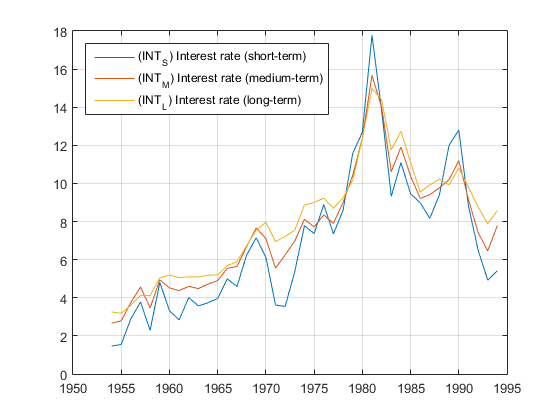
\includegraphics[width=1\textwidth]{TestMultipleSeriesForCointegrationUsingJcitestExample_01}
        \caption{Cointegration of the interest rates (short, medium and long-term) in Canada from 1955 to 1995}
        \label{TestMultipleSeriesForCointegrationUsingJcitestExample_01}
    \end{subfigure}
    \begin{subfigure}[t]{0.49\textwidth}
        \centering
        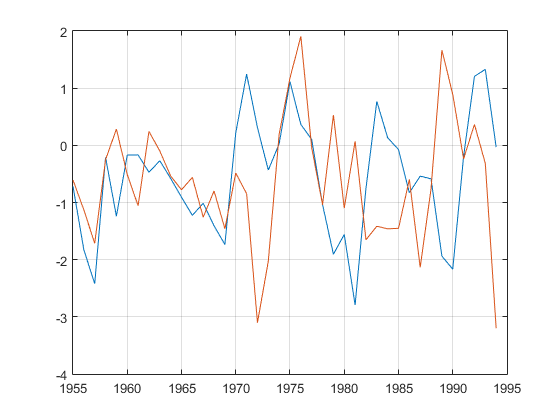
\includegraphics[width=1\textwidth]{TestMultipleSeriesForCointegrationUsingJcitestExample_02}
        \caption{Estimated Cointegrating relations $\beta' y_{t-1} + c_0$}
        \label{TestMultipleSeriesForCointegrationUsingJcitestExample_02}
    \end{subfigure}
    \caption{Cointegration property of the Canadian interest rates}
\end{figure}

It seems that the existence of more than one cointegrating vector (i.e. the long-run relationship) is not necessarily a good sign, since there is uncertainty as to which relationship the variables will obey in the long and short run. The dynamics may be unstable. The assumption will be discussed later.

\section{Testing for Unit Roots in Stochastic Processes}
\label{sec:unit_root_testing}
% PP TEST doc very interesting
Before testing for a unit root, (i.e. if the series is $I(1)$), the time series must be transformed to its linear form. Usually, assets prices have an exponential growth and logarithm should be applied accordingly to satisfy this prerequisite. Once the data is transformed, we have to choose the most pertinent model to use in the Augmented Dickey Fuller test. This test is an enhanced version of the Dickey-Fuller test, which assesses the presence of a unit root in an autoregressive model. The augmented version has a larger and more complicated set of time series models. There are three basic models for economic data $\matr{Y}_t$
%http://uk.mathworks.com/help/econ/adftest.html#inputs
\begin{itemize}
\item Trend Stationary model variant (TS) \\
H0: $y_t = c + y_{t-1} + \phi_1 \Delta y_{t-1} + \cdots + \phi_p \Delta y_{t-p} + \epsilon_t $ \\
H1: $y_t = c \delta t + \gamma y_{t-1} + \phi_1 \Delta y_{t-1} + \cdots + \phi_p \Delta y_{t-p} + \epsilon_t $ \\
with drift coefficient $c$, deterministic trend coefficient $\delta$ and $AR(1)$ coefficient $\gamma <1$.
\item Auto Regressive with Drift variant (ARD) \\
H0: $y_t = y_{t-1} + \phi_1 \Delta y_{t-1} + \cdots + \phi_p \Delta y_{t-p} + \epsilon_t $ \\
H1: $y_t = c + \gamma y_{t-1} + \phi_1 \Delta y_{t-1} + \cdots + \phi_p \Delta y_{t-p} + \epsilon_t $ \\
with drift coefficient $c$, and $AR(1)$ coefficient $\gamma <1$.
\item Auto Regressive variant (AR) \\
H0: $y_t = y_{t-1} + \phi_1 \Delta y_{t-1} + \cdots + \phi_p \Delta y_{t-p} + \epsilon_t $ \\
H1: $y_t = \gamma y_{t-1} + \phi_1 \Delta y_{t-1} + \cdots + \phi_p \Delta y_{t-p} + \epsilon_t $ \\
with $AR(1)$ coefficient $\gamma <1$.
\end{itemize}

%http://uk.mathworks.com/help/econ/unit-root-nonstationarity.html Choose Models to Test
$\epsilon_t$ is a mean zero innovation process. In general, if the series is growing, the TS model provides a reasonable trend-stationary alternative to a unit-root process with drift. If the series shows no trend but has a non zero mean, the ARD model provides reasonable stationary alternatives to a unit-root process without drift. Finally, if the series has no trend and a zero mean, the AR model is the most suitable. As the spread is a non zero mean without any drift, the ARD model is the best alternative model for testing. \\

%https://tel.archives-ouvertes.fr/hal-01020405/document
The next step is to determine the number of lags to include in the model. Different criteria used for lag length often lead to different decisions regarding the optimal lag order that should be used in the model. \cite{daoimpact} suggested a general procedure for the ADF test
\begin{itemize}
\item Determine the optimal max lag value denoted $L_{max}$. It is clear that $L_{min} = 0$ is the minimum value of lag length that could be used. \cite{schwert2002} suggested to use $L_{max} = 12 \left(T / 100 \right)^{1/4}$ where $T$ is the length of the time series. It guarantees that $L_{max}$ grows with $T$.
\item When $L_{min}$ and $L_{max}$ are established, ADF t-statistics are calculated for all lag length values between the range $(L_{min}, L_{max})$. The most negative value from all ADF t-statistics indicates the value of lag length that produces the most stationary residuals.
\end{itemize}
% The general method to find the optimal lag for the Phillips-Perron test is to begin with few lags, and then evaluate the sensitivity of the results by adding more lags. Another rule of thumb is to look at sample autocorrelations of $\Delta y_t = y_t - y_{t-1}$. Slow rates of decay require more lags. It is less suitable for economic data because it is widely known that the returns $\Delta y_t$ show no autocorrelation. Finally, when the optimal lags are known, multiple tests are run to avoid any possible inconsistency.

\section{Creation and Validation of the Spread Instruments}
A rigorous testing for cointegration is performed to select the tuples for trading. It involves Johansen, Augmented Dickey Fuller and Variance Ratio tests. The Variance Ratio Test (VRT) is based on the idea that a stationary series does not have its variance increasing with time. \\

Algorithm \ref{formation_spread_algorithm} explains the procedure. The result of a test is denoted $h = p_{value} < 0.05$. Values of $h$ equal to 1 indicate rejection of the null hypothesis in favor of the alternative model. Values of $h$ equal to 0 indicate a failure to reject the null.

\begin{algorithm}[H]
\caption{Formation of the Spread}\label{formation_spread_algorithm}
\begin{algorithmic}[1]
\Procedure{CreateSpread}{$M$ tuples of size $N$ : $\{ (\matr{X}_i)_{1 < i \leq N} \}_{m}$}
\For{m from 1 to M}
  \State Select the tuple $(\matr{X}_i)_{1 < i \leq N}$ indexed by $m$
  \For{i from 1 to N}
    \State h = Test $\matr{X}_i \sim I(1)$ with an Augmented Dickey-Fuller test
	  \If{h = 1 ($\matr{X}_i \not\sim I(1)$)}
      \State \textbf{Break}
    \EndIf
  \EndFor{end}
  
  \State $[h_1,...,h_N]$ = Perform Johansen Cointegration Test on $(\matr{X}_i)_{1 < i \leq N}$
  \State $r$ = Determine Cointegration Rank of $[h_1,...,h_N]$
  
  \If{$r \neq 1$} //One cointegrating relation is enough
    \State \textbf{Break}
  \EndIf
  
  \For{j from 1 to N} //Order is important in a tuple
    \State Regress $\Delta \matr{X}_j = f((\Delta \matr{X}_i)_{i \neq j})$
    \State Form the spread $\matr{S} = \beta'\matr{X} = \matr{X}_j - \sum_{i\neq j} \beta_i \matr{X}_i$
    \State Determine the optimal lag $p$ for the ADF test (Section \ref{sec:unit_root_testing})
    \State $h_1$ = Test $\matr{S} \sim I(1)$ with an Augmented Dickey-Fuller test with lags $[0,p]$
    \State $h_2$ = Test $\matr{S} \sim RW(\cdot)$ with variance ratio test for random walk
    \If{$h_1 = 1$ \textbf{and} $h_2 = 1$}
      \State $\matr{S}$ is a spread candidate for trading. Add to list $\mathcal{L}$
      \State \textbf{Break} //Success. Go to next tuple.
    \EndIf
  \EndFor{end} \\
\EndFor{end}

\\
\Return $\mathcal{L}$ : list of cointegrated spreads
\EndProcedure
\end{algorithmic}
\end{algorithm}

\chapter{State-Space Models and Stochastic Volatility}
\section{State-Space Models}
\label{section:ssm}
The term \textit{state-space} originated in 1960s in the area of control engineering (\cite{kalman1960}). State-space models refers to a class of probabilistic graphical model that describes the probabilistic dependence between the latent state variables $\matr{x}_{1:T}$ and the observed measurements $\matr{y}_{1:T}$. The system evolves according to
\begin{align*}
\matr{X}_t &= f_\theta(\matr{X}_{t-1},\matr{W}_{t-1}) \numberthis \label{system_equation} \\
\matr{Y}_t &= h_\theta(\matr{X}_t, \matr{V}_t) \numberthis \label{measurement_equation}
\end{align*}
where, $\matr{X}_t \in \mathbb{R}^n$ is the state vector and $\matr{Y}_t \in \mathbb{R}^n$ is the measurement vector. $f_\theta$ is a Markov process of order one and $h_\theta$ is any non-linear function. Both $f_\theta$ and $h_\theta$ are assumed to be time invariant and deterministic. $\matr{W}_t$ and $\matr{V}_t$ are respectively the i.i.d. system and i.i.d. measurement noise sequences. The Directed Acyclic Graph (DAG) for this state-space is given in Figure \ref{state_space_models}. \\

Equation (\ref{system_equation}) is known as the system equation and Equation (\ref{measurement_equation}) is known as the measurement equation.  We assume that the process generating the system states $\matr{X}_t$ and thus the observed states $\matr{Y}_t$ starts from an initial value $\matr{x}_1$. The joint process $(\matr{W}_t, \matr{V}_t)$ is a zero mean, serially uncorrelated noise process with possibly time varying covariance matrices
\begin{equation}
\begin{pmatrix}
\Sigma_{\matr{W}_t} & \Sigma_{\matr{W}_t, \matr{V}_t}\\
\Sigma_{\matr{V}_t, \matr{W}_t} & \Sigma_{\matr{V}_t} \label{corr_ssm}
\end{pmatrix}
\end{equation}
It is worth mentioning that some models make additional assumptions about the noise processes.
\begin{figure}[H]
\centering
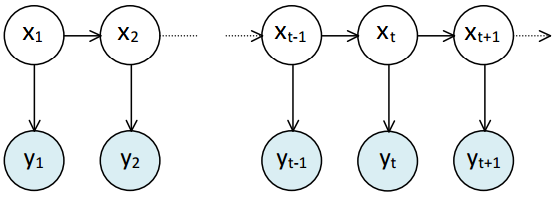
\includegraphics[width = 0.75\textwidth]{state_space_models}
\caption{DAG for the state-space model with first order Markov latent dynamics}
\label{state_space_models}
\end{figure}

The functions $f_\theta$ and $h_\theta$ are parametrized by $\theta = (\theta_1,...,\theta_n)^T$ and each $\theta_i$ is assumed to be independent from $(\theta_j)_{j \neq i}$. A joint prior distribution $p(\theta) = \prod_i p(\theta_i)$ is specified. With the assumptions mentioned above, the probability density of $\matr{x}_{1:T}$ is written as
\begin{equation}
p(\matr{x}_{1:T} | \theta) = p(\matr{x}_1|\theta) \prod_{t=2}^T p(\matr{x}_t|\matr{x}_{t-1}, \theta) 
\end{equation}

The realization $\matr{x}_{1:T}$ is not observed directly, but through $\matr{y}_{1:T}$. The state-space model assumes that each observation $\matr{y}_t$ is statistically independent of every other quantity except $\matr{x}_t$ and $\theta$, through Equation (\ref{measurement_equation}). As a consequence, the conditional likelihood of the observations, given the state process can be derived as
\begin{equation}
p(\matr{y}_{1:T} | \matr{x}_{1:T}, \theta) = \prod_{t=2}^T p(\matr{y}_t | \matr{x}_t, \theta) = \int p(\matr{y}_T|\matr{x}_T, \theta) d\matr{y}_T
\end{equation}
where $d \matr{y}_T$ is the Lebesgue measure. Here, $\theta$ is treated as unknown and the general idea is to estimate it using Maximum Likelihood Estimation (MLE) on the marginal likelihood $p(\matr{y}_{1:T}|\theta)$, with the latent variables $\matr{x}_{1:T}$ integrated out
\begin{equation}
p(\matr{y}_{1:T} | \theta) = p(\matr{y}_1 |\theta) \prod_{t=2}^T p(\matr{y}_t | \matr{y}_{1:t-1}, \theta) = \int p(\matr{y}_T|\matr{x}_T, \theta) p(\matr{x}_T|\matr{y}_{1:T-1}, \theta) d \matr{x}_T\label{intractable_ssm_2}
\end{equation}
It is also worth considering the approximation of the latent variables $p(\matr{x}_{1:T}, \theta | \matr{y}_{1:T})$. By Bayes theorem,
\begin{align*}
p(\matr{x}_{1:T}, \theta | \matr{y}_{1:T}) &= \frac{ p(\theta)p(\matr{x}_{1:T}|\theta)p(\matr{y}_{1:T}|\matr{x}_{1:T}, \theta) }{p(\matr{y}_{1:T})}\numberthis \label{intractable_ssm}
\end{align*}
where
\begin{equation}
p(\matr{y}_{1:T}) = \int p(\matr{y}_{1:T}|\theta')p(\theta') d\theta' = \iint p(\matr{y}_T|\matr{x}_T, \theta') p(\matr{x}_T|\matr{y}_{1:T-1}, \theta') p(\theta') d \matr{x}_T d\theta'
\end{equation}

In most cases, $p(\matr{x}_{1:T}, \theta | \matr{y}_{1:T})$ is hard to compute because $p(\matr{y}_{1:T} | \theta)$ is analytically intractable. When $\theta$ is known, the problem of inference in the path space is effectively addressed using Sequential Monte Carlo methods. However, despite the success of standard SMC methods, the general case of the joint inference on $\theta$ and on $\matr{x}_{1:T}$ for a generic non-linear non-Gaussian state-space model is a very challenging problem, which, although extremely important for a wide variety of applications, is still somewhat unresolved. To attempt to overcome these difficulties, \cite{andrieu2010} developed \textit{Particle Markov Chain Monte Carlo} algorithms. These are MCMC algorithms which use a particle filter to estimate the intractable true value of (\ref{intractable_ssm_2}). This framework is presented in more depth in Section \ref{section:pmcmc}.

\section{Stochastic Volatility Models}
\label{sec:sv}
The most important feature of the conditional return distribution $Y_t | \mathcal{F}_{t-1}$ is its variance dynamics. The first research on modelling this volatility was \cite{engle1982} with the famous heteroskedastic ARCH model. The main objective was to fit the fat tails of the return distributions and deal with volatility clustering. This section presents more recent models known as Stochastic Volatility models. The intrinsic feature of the SV model is that each observation $y_t$ is assumed to have its own variance. In order to have a realistic model, this variance is not allowed to vary unrestrictedly with time. Rather, its logarithm is assumed to follow an autoregressive process of order one. It is worth noting that this feature is fundamentally different to GARCH models where the time-varying volatility is assumed to follow a deterministic instead of a stochastic evolution.

\subsection{Model $\mathcal{M}_1$ - Standard Stochastic Volatility Model (SV)}
The standard discrete-time SV model for the returns $Y_t$ is defined as
\begin{align*}
  X_t &=  \phi X_{t-1} + \sigma \epsilon_{X,t-1} \numberthis \label{std_SV_process_X} \\
  Y_t &=  \beta \exp \left( \frac{X_t}{2} \right) \epsilon_{Y,t} \numberthis
\end{align*}
where $\epsilon_{X,t}, \epsilon_{Y,t}$ are two independent and standard normally distributed processes. Let $\theta = (\rho, \sigma, \beta)$ be the parameters vector. This model is non-linear because of the nature of $h_\theta$. $X_t$ governs the volatility process of the observed returns $Y_t$, $\sigma$ is the volatility of the volatility, $\phi$ the persistence parameter of $X_t$, and $\beta$ is a scaling parameter. The condition $|\phi| < 1$  is imposed to have a stationary process, with initial condition $X_0 \sim \mathcal{N} \left(0, \frac{\sigma^2}{1-\phi^2} \right)$, where $\frac{\sigma^2}{1-\phi^2}$ is the unconditional variance of $X_t$. The next part explains the link between the stochastic volatility model and the Geometric Brownian Motion (GBM).

%https://en.wikibooks.org/wiki/LaTeX/Theorems
\begin{definition}
\textit{
A stochastic process $S_t$ is said to follow a Geometric Brownian Motion if it satisfies the following stochastic differential equation
$dS_t = \mu S_t dt + \sigma S_t dW_t$
where $W_t$ is a Wiener process, $\mu$ the drift and $\sigma$ the volatility. Both $\mu$ and $\sigma$ are assumed to be constant.}
\end{definition}

The process can be discretized by
\begin{align*}
S_{t+1}-S_t &= \mu S_t + \sigma S_t \epsilon_{t+1} \text{, } \epsilon_{t} \sim \mathcal{N}(0,1) \\
S_{t+1} 	&= S_t + \mu S_t + \sigma S_t \epsilon_{t+1} \\
S_t 	&= S_{t-1} + \mu S_{t-1} + \sigma S_{t-1} \epsilon_t \numberthis
\end{align*}

In the Stochastic Volatility model, $Y_t$ represents the returns of the modelled asset. A general definition for computing the returns is $y_t = S_t / S_{t-1} - 1$, where $S_t$ is the observed prices of the asset. When $x_t$ is measured at time $t-1$ with regard to the filtration $\mathcal{F}_{t-1}$, $Y_t | x_t, \theta$ is normally distributed as
\begin{align*}
Y_t | x_t, \theta 					&\sim \mathcal{N}(0, \beta^2 \exp(x_t)) \\
S_t | x_t, \theta 					&\sim \mathcal{N}(S_{t-1}, \underbrace{S_{t-1}^2 \beta^2 \exp(x_t)}_{\sigma^2(t)}) \numberthis \label{cond_dist_sv_model}
\end{align*}

The variance $\sigma^2(t)$ always exists as a product of square and exponential terms. Finally, Equation \ref{cond_dist_sv_model} can be rewritten as $S_t = S_{t-1} + \sigma(t) S_{t-1} \epsilon_t \text{, } \epsilon_t \sim \mathcal{N}(0,1)$ which corresponds to the discretized Geometric Brownian Motion equation with $\mu = 0$ if and only if $\sigma(t) = \sigma \text{, } \forall t > 0$. The interest of using a Stochastic Volatility model essentially relies on the ability of modelling this volatility.

\subsection{Model $\mathcal{M}_2$ - Stochastic Volatility Student-t (SVt)}
The first extension is a stochastic volatility model with heavier tails where $\epsilon_{Y,t} \sim t(\nu)$. $\theta$ is enriched with the new parameter $\nu$, supposed to be unknown.

\begin{lemma}
\textit{
Assume that $X$ is a random variable of probability density function $f_X(x)$. The probability density function $f_Y(y)$ of $Y=g(X)$ where $g$ is monotonic, is given by
}
\begin{equation}
f_Y(y) = \left|\frac{d}{dy}(g^{-1}(y))\right| \cdot f_X(g^{-1}(y))
\end{equation}
\end{lemma}


Applying this lemma on $y_t = \sigma(t) \epsilon_{Y,t}$ where $\sigma(t) = \beta \exp \left(\frac{x_t}{2} \right)$ and $g^{-1}_t(x) = \frac{x}{\sigma(t)}$ gives,

\begin{equation}
p(y_t | x_t, \theta) = \frac{\Gamma(\frac{\nu+1}{2})}{\Gamma(\frac{\nu}{2}) \sqrt{\nu\pi}} \frac{1}{\sigma_t}\left( 1 + \frac{y_t^2}{\sigma_t^2 \nu}\right)^{-\left(\frac{v+1}{2} \right)}
\end{equation}
where $\Gamma(\cdot)$ is the gamma function. This result can also be retrieved by considering the $t$ location-scale distribution with parameters $(\mu = 0, \sigma, \nu)$, whose probability density function is given by
\begin{equation}
p(x,\sigma,\nu,\mu) = \frac{\Gamma \left(\frac{\nu+1}{2} \right)}{\sigma \sqrt{\pi \nu} \Gamma \left(\frac{\nu}{2} \right)} \left[ \frac{\nu + \left( \frac{x-\mu}{\sigma}\right)^2}{\nu}\right]^{-\left(\frac{\nu+1}{2} \right)}
\end{equation}


The reasoning to find a closed form of $(S_t | x_t, \theta)$ is similar to the standard stochastic volatility model. Still under the assumption that $\epsilon_{Y,t} \sim t(\nu)$, if $X$ has a $t$ location-scale distribution, with parameters $\mu, \sigma, \nu$, then $\frac{X-\mu}{\sigma}$ has a Student's $t$ distribution with $\nu$ degrees of freedom. Reverting the equation yields $X = \mu + \sigma \epsilon_{Y,t}$. Consequently,
\begin{align*}
S_t  &= \underbrace{S_{t-1}}_{\mu(t)} + \underbrace{\beta |S_{t-1}| \exp \left( \frac{x_t}{2} \right)}_{\sigma(t)} \epsilon_{Y,t} \numberthis
\end{align*}
Because the spread $S_t$ can be negative, the absolute value $|.|$ is considered to ensure that $\sigma(t)$ is always positive definite. As a conclusion, $S_t | x_t, \theta$ follows a $t$ location-scale distribution of parameters $(\mu(t), \sigma(t), \nu)$. 

\subsection{Model $\mathcal{M}_3$ - Stochastic Volatility Leverage (SVL)}
In the second extension, a leverage effect is added. \cite{black1976} discovered that most measures of volatility of an asset are negatively correlated with the returns of that asset. It is considered nowadays as a stylized fact in econometrics series. Let $\rho$ denote the correlation between the innovation processes $\epsilon_{X,t}$ and $\epsilon_{Y,t}$. $\theta$ is enriched with the new parameter $\rho$.

\begin{lemma}
\textit{
[Cholesky Decomposition] Let $X$, $Y$ be two standard normally distributed random variables. The correlation between X and Y is $\rho$ if and only if $Y = \rho X + \sqrt{1-p^2} Z$ where $Z \sim \mathcal{N}(0,1)$ and is independent of both $X$ and $Y$.
}
\end{lemma}
Applying the Cholesky decomposition on the innovations gives $\epsilon_{X,t} = \rho \epsilon_{Y,t} + \sqrt{1-\rho^2} Z$. This identity is helpful when it comes to generate artificial datasets from this model. Recall that $\epsilon_{Y,t}$ is first measured ($\mathcal{F}_{t-1}$-measurable) and $\epsilon_{X,t}$ is updated accordingly ($\mathcal{F}_t$-measurable). It means that $\epsilon_{Y,t}$ is independent from all the past values $(\epsilon_{X,s})_{s < t}$. Consequently, the conditional distributions of $Y_t$ and $S_t$ remain unchanged from Equation (\ref{cond_dist_sv_model}).

%http://people.anu.edu.au/joshua.chan/Chan-Hsiao-2013.pdf
\subsection{Model $\mathcal{M}_4$ - Stochastic Volatility Moving Average (SVMA)}
The standard stochastic volatility model assumes that the errors in the measurement equation are serially independent. This is often an appropriate assumption for modelling financial data. To test this assumption, the plain model can be extended by allowing the errors in the measurement equation to follow a moving average (MA) process of order $m$. Here, we choose a simple specification and set $m = 1$. Hence, our model becomes
\begin{align*}
Y_t							      &= \beta \exp \left( \frac{X_t}{2} \right) \epsilon_{Y,t} + \psi \beta \exp \left( \frac{X_{t-1}}{2} \right) \epsilon_{Y,t-1} \numberthis \\
Y_t	| \mathcal{F}_{t-1}		&\sim \mathcal{N} \left(0, \beta^2 \exp \left( x_t \right) + \psi^2 \beta^2 \exp \left( x_{t-1} \right) \right) \\
S_t | \mathcal{F}_{t-1}	  &\sim \mathcal{N} \left(S_{t-1}, S_{t-1}^2 \beta^2 \exp \left( x_t \right) +  S_{t-1}^2 \psi^2 \beta^2 \exp \left( x_{t-1} \right) \right) \numberthis
\end{align*}
where the process $X$ is defined in Equation (\ref{std_SV_process_X}). As before, we ensure that the root of the characteristic polynomial associated with the MA coefficient $\psi$, is outside the unit circle: $|\psi| < 1$. When $\psi = 0$, the SV-MA(1) model is reduced to the standard stochastic volatility model. The conditional
variance of $Y_t$ is given by $\var \left(Y_t | \mathcal{F}_{t-1} \right) = \beta^2 e^{x_t} + \beta^2 \psi^2 e^{x_{t-1}}$. The conditional variance is time-varying through two channels: a moving average composed of the two most recent variances $\beta^2 e^{x_t}$ and $\beta^2 e^{x_{t-1}}$ and secondly, according to the stationary $AR(1)$ process $X_t$.

\subsection{Model $\mathcal{M}_5$ - Stochastic Mean (SVM)}
\cite{koopman2002} suggested an extension where the stochastic volatility also enters into the conditional mean equation. This model is known as the Stochastic Volatility in Mean (SVM). It is defined as
\begin{align*}
Y_t 			 &= \beta \exp\left(\frac{X_t}{2}\right) + \exp\left(\frac{X_t}{2}\right) \epsilon_{Y,t} \numberthis\\
S_t | \mathcal{F}_{t-1}  &\sim \mathcal{N} \left(S_{t-1} + S_{t-1} \beta \exp\left(\frac{x_t}{2}\right), S_{t-1}^2 \exp\left(x_t\right) \right) \numberthis
\end{align*}
where $X_t$ corresponds to the process of a standard stochastic volatility model defined in Equation (\ref{std_SV_process_X}). This model is pertinent if we believe that the conditional mean is somehow proportional to the conditional volatility.

\subsection{Model $\mathcal{M}_6$ - Two Factors Stochastic Volatility (TFSV)}
\cite{chernov2000} found that SV models with one volatility factor are not able to characterize all moments of asset return distributions. In particular, the fat tails of the return distribution are captured rather poorly. With a principal component analysis, \cite{harvey1994} showed that a short-run and a long-run factors might be enough to explain the volatility of the returns. The study was performed on daily observations on several exchange rates. This model is known as the two factor stochastic volatility and relies on two different latent processes $X$ and $Z$. It is defined as
\begin{align*}
  X_t 						&=  \phi_X X_{t-1} + \sigma_X \epsilon_{X,t-1} &|\phi_X| < 1, \epsilon_{X,t-1} \sim \mathcal{N}(0,1), X_1 \sim \mathcal{N} \left(0, \frac{\sigma_X^2}{1 - \phi_X^2} \right) \numberthis \label{tfsv_process_X} \\
  Z_t 						&=  \phi_Z Z_{t-1} + \sigma_Z \epsilon_{Z,t-1} &|\phi_Z| < 1, \epsilon_{Z,t-1} \sim \mathcal{N}(0,1), Z_1 \sim \mathcal{N} \left(0, \frac{\sigma_Z^2}{1 - \phi_Z^2} \right) \numberthis\\
  Y_t 						&=  \beta \exp \left( \frac{X_t+Z_t}{2} \right) \epsilon_{Y,t} &\epsilon_{Y,t} \sim \mathcal{N}(0,1) \numberthis
\end{align*}
Under these assumptions, the conditional distribution of the spread is $S_t | x_t, z_t, \theta \sim \mathcal{N}\left(S_{t-1}, S_{t-1}^2 \beta^2 \exp \left(x_t + z_t\right) \right)$. The parameters vector $\theta$ is now $(\beta, \phi_X, \phi_Z, \sigma_X, \sigma_Z)$. It is of common knowledge that the returns are leptokurtic, i.e. with a positive kurtosis. \cite{veiga2006} showed that the second term introduced in the model helps generate extra kurtosis and accounts for short-run dynamics.

\subsection{Model $\mathcal{M}_7$ - Two Factors Stochastic Volatility with Leverage (TFSVL)}

In the final extension, we consider the two factors stochastic volatility with a correlation $\rho = corr(\epsilon_{X,t}, \epsilon_{Y,t})$. The idea is the same as the one developed for the model $\mathcal{M}_3$. We assume a non-zero correlation between the innovations of the returns and the long-run factor $X$ from Equation (\ref{tfsv_process_X}). From the models presented before, this model is by far the most complex because 6 parameters are to be estimated: $\beta, \rho, \phi_X, \phi_Z, \sigma_X$ and $\sigma_Z$. \cite{ruiz2008} studied a slightly different version with $X_t$ defined as a fractional integrated Gaussian noise process (ARFIMA). They proved that the first order autocorrelation $corr(|y_t|,|y_{t+1}|)$ is smaller than the second order autocorrelation $corr(y_t^2,y_{t+1}^2)$ when $\rho < 0$. As explained by \cite{cont2005}, it is usually the case in practical applications. From the same considerations as in model $\mathcal{M}_3$, the conditional distributions of $Y_t$ and $S_t$ remains unchanged compared to model $\mathcal{M}_6$.

\chapter{Sequential Monte Carlo and Particle Markov Chain Monte Carlo}
\label{section:pmcmc}
\section{From SMC to PMCMC in Nonlinear Filtering}
Many problems involve making inference on unknown parameters of complex models which have a sequential, if not explicitly temporal, basis. In the first part, Sequential Monte Carlo (SMC) methods are introduced followed by a presentation of the Particle Marginal Metropolis Hastings (PMMH), an implementation of the Particle MCMC scheme. This chapter keeps the same notations as in Chapter \ref{section:ssm} where the state-space models are defined.\\

\textit{Sequential Monte Carlo} (SMC) are a collection of simulation-based techniques to address nonlinear filtering problems arising in signal processing and Bayesian statistical inference. The filtering problem consists in estimating the latent states $\matr{x}_{1:T}$ when only the observations $\matr{y}_{1:T}$ are known. The objective of SMC is to compute a recursive series of posterior distributions over such complex models. SMC methods are very flexible, relatively easy to implement and parallelizable. Since computational resources have become so readily available, and due to certain recent advanced in applied statistics, these methods have recently become a mainstay of advanced research methods in this field.\\

\textit{Particle Markov Chain Monte Carlo} (Particle MCMC) are powerful techniques for estimating parameters of a complex model where classical methods are limited. Examples of complex models include state-space models with latent variables. The main feature behind Particle MCMC is the use of a particle filter of size $N$ inside a MCMC scheme. This filter provides estimates of the intractable marginal likelihood $p(\matr{y}_{1:T}|\theta)$.

\section{Monte Carlo Methods}
\label{section:mc}
Sequential Monte Carlo (also known as Particle Filtering) paradigm is based on Monte Carlo methods such as rejection sampling and importance sampling. This section introduces both of them briefly.

\subsection{Rejection Sampling}
Rejection sampling is a technique which samples from a target distribution $p(\matr{X})$ (known up to a proportional constant) by sampling from another easy to sample proposal distribution $\pi(\matr{X})$. This assumes that there exists a known finite constant $C$ such that $p(\matr{X}) \leq C \pi(\matr{X})$ for every $\matr{x}$. The idea is to draw $\matr{X} \sim \pi$ and accept it as a sample of $p$ with probability $p(\matr{X}) / ( C \pi(\matr{X}))$.

\subsection{Importance Sampling}
The idea of importance sampling is to choose a proposal distribution $\pi(\matr{X})$ in place of the true probability distribution $p(\matr{X})$, which is difficult to sample. The support of $\pi(\matr{X})$ is assumed to cover that of $p(\matr{X})$. Under these assumptions, the classic Monte Carlo integration problem is
\begin{equation}
p(f) = E[f(\matr{X})] = \int f(\matr{X})p(d\matr{X})
\end{equation}
for any suitable function $f$. It can be rewritten as
\begin{equation}
\int f(\matr{X})p(\matr{X})d\matr{X} = \int f(\matr{X}) \frac{p(\matr{X})}{\pi(\matr{X})} \pi(\matr{X}) d\matr{X} \label{is_equation}
\end{equation}
Importance sampling is used to draw a number of independent samples from $\pi(\matr{X})$ to obtain an estimate of Equation (\ref{is_equation}). Each sample, $f(\matr{X}_i)$ is assigned an importance weight, $W(\matr{X}_i) \propto p(\matr{X}_i)/\pi(\matr{X}_i)$. In practice, the variance of the importance weights must be finite and the proposal distribution $\pi(\matr{X})$ should be as close to possible to $p(\matr{X})$ such that the variance of the weights is minimized. 

\section{Sequential Monte Carlo Methods}
\label{section:smc}
\subsection{Sequential Importance Sampling Resampling}
The Sequential Importance Sampling Resampling (SIS-R) algorithm is a sequential version of importance sampling with resampling which approximates the filtering probability density $p(\matr{x}_t|y_{1:t})$ of the latent variables by a weighted set of $N$ samples $(w_t^{(i)}, \matr{x}_t^{(i)})_{1 \leq i \leq N}$, where $N$ is the number of particles. The importance weights $w_t^{(i)}$ are the approximations to the relative posterior distributions. This algorithm has been introduced in 1987 to tackle the degeneracy problem, unresolved by its previous version, known as Sequential Importance Sampling (SIS). The degeneracy happens when all but one of the importance weights are close to zero. The correction is done by adding a resampling step to eliminate samples with trivial importance weights and propagate particles with larger weights. As in importance sampling, the expectation of a function $f$ can be approximated as a weighted average
\begin{equation}
\int f(\matr{x}_t)p(\matr{x}_t|y_{1:t})d \matr{x}_t \simeq \sum_{i=1}^N w_t^{(i)} f(\matr{x}_t^{(i)})
\end{equation}

This step is presented in Algorithm \ref{algo_resampling_step}. The input is the set of particles at time $t$ and the output is this same set resampled with the weights being re-initialized. $N$ is the number of particles in the particle filter.
\begin{algorithm}[H]
\caption{Multinomial Resampling}\label{algo_resampling_step}
\begin{algorithmic}[1]
\Procedure{MultinomialResampling}{$(w_t^{(i)}, \matr{x}_t^{(i)})_{1 \leq i \leq N}$, $N$}
\For{i from 1 to N}
  \State Sample an integer $j \in [1,N]$ with probabilities proportional to $\{w_{t}^{(1)},..., w_{t}^{(N)}\}$
  \State Replace the current particle $i$ with this new one. $\matr{x}_t^{(i)} \gets \matr{x}_t^{(j)}$
  \State Re initialize the weight $w_t^{(i)} = 1/N$
\EndFor{end}
\EndProcedure
\end{algorithmic}
\end{algorithm}

The general algorithm SIR is presented in Algorithm \ref{algo_sisr_filter}. The input consists in the observations $y_{1:T}$, the parameters vector $\theta$ and the number of particles $N$. The output is the estimated latent states $\matr{x}^*_{1:T}$ and the estimator $\hat{p}^N_\theta(y_{1:T})$. Generally, the resampling step is not performed at each time but at some specific steps to improve the performance. It is controlled by the Effective Sample Size (ESS) parameter which gives an estimate of the effective number of particles. When it is too low, it means that the algorithm is performing poorly and a resampling is necessary. A threshold $N_{thr}$ is arbitrary selected to trigger this resampling. Usually, it is equal to $N/3$ but can vary depending on the applications.

\begin{algorithm}[H]
\caption{Sequential Importance Sampling Resampling (SISR)}\label{algo_sisr_filter}
{\small
\begin{algorithmic}[1]
\Procedure{SISR}{$y_{1:T}$, $\theta$, N, $N_{thr}$}
\For{i from 1 to N}
	\State Sample $\matr{x}_1^{(i)} \sim \pi (\matr{x}_1)$
	\State Calculate weight $w_1^{(i)} = \displaystyle{\frac{p(y_1 | \matr{x}_1) p(\matr{x}_1)}{\pi (\matr{x}_1 | y_{1:t})}}$
\EndFor{end}
\State $\matr{x}^*_1 = \sum_{i=1}^N \matr{x}_1^{(i)}.w_1^{(i)}$
\State Set $\hat{p}^N_\theta(y_1) = \frac{1}{N} \sum_{i=1}^N w_1^{(i)}$

\For{t from 2 to T}
	\For{i from 1 to N}
	  \State Draw sample from the proposal distribution $\matr{x}_t^{(i)} \sim \pi \left(\matr{x}_t|\matr{x}_{1:t-1}^{(i)}, y_{1:t} \right)$
		\State Calculate weight $\displaystyle{\hat{w}_t^{(i)} = w_{t-1}^{(i)} \frac{p(y_t|\matr{x}_t^{(i)}) p(\matr{x}_t^{(i)}|\matr{x}_{t-1}^{(i)})}{\pi \left(\matr{x}_t^{(i)}|\matr{x}_{1:t-1}^{(i)}, y_{1:t} \right)}}$
	\EndFor{end}
	\State Compute the normalized importance weight for each $i$, $\displaystyle{w_t^{(i)} = \frac{\hat{w}_t^{(i)}}{\sum_{j=1}^N \hat{w}_t^{(j)}}}$
	\State Compute the ESS as $N_{eff} = 1 / \left(  \sum_{i=1}^N \left(w_t^{(i)} \right)^2 \right)$
	\If{$N_{eff} < N_{thr}$} 
		  \State //perform resampling step
		\EndIf{end}
	\State $\matr{x}^*_t = \sum_{i=1}^N \matr{x}_t^{(i)}.w_t^{(i)}$
	\State Set $\hat{p}^N_\theta(y_{1:t}) = \hat{p}^N_\theta(y_{1:t-1}) \left(\frac{1}{N} \sum_{i=1}^N w_t^{(i)} \right)$
\EndFor{end}
\\
\Return ($\matr{x}^*_{1:T}$, $\hat{p}^N_\theta(y_{1:T})$)
\EndProcedure
\end{algorithmic}
}
\end{algorithm}

It is worth noting that $\matr{x}$ can be multivariate. Models exist where the observations are generated from two or more latent processes (models $\mathcal{M}_6$ and $\mathcal{M}_7$ are such examples). In the case where $\matr{x}$ is bivariate, the particle filter is updated to draw two sets of particles instead of one (one for $\matr{x}_1$ and one for $\matr{x}_2$). \\

Particle filters with transition prior probability distribution $f_\theta$ as importance function $\pi(\matr{X})$ are commonly known as Bootstrap filter. This choice is motivated by the facility of drawing particles and performing subsequent importance weight calculations. Here, $\pi(\matr{x}_t| \matr{x}_{1:t-1}, y_{1:t}) = p(\matr{x}_t |\matr{x}_{1:t-1}, y_{1:t})$. Coupled with a resampling done at each step, set by $N_{thr} = \infty$, the weights formula is simplified to
\begin{equation}
w_t^{(i)} = \frac{p(y_t|\matr{x}_t^{(i)})p(\matr{x}_t^{(i)}|\matr{x}^{(i)}_{t-1})}{\pi(\matr{x}_t^{(i)}|\matr{x}^{(i)}_{1:t-1},y_{1:t})}=  p(y_t|\matr{x}_t^{(i)})
\end{equation}

It is clear from the understanding of importance resampling that these weights are appropriate for representing a sample from $p(\matr{x}_t|y_{1:t})$, and so the particles and weights can be propagated forward to the next time point. It is also clear that the average weight at each time gives an estimate of the marginal likelihood of the current data point given the data so far. So we define the conditional marginal of $y_t$ by

\begin{equation}
 \hat{p}^N_{\theta}(y_t | y_{1:t-1}) = \frac{1}{N} \sum_{k=1}^N w_t^k
\end{equation}

and the conditional marginal estimator of $y_{1:T}$ over all the state-space is
\begin{equation}
 \hat{p}^N_\theta(y_{1:T}) = \hat{p}^N_\theta(y_1)\prod_{t=2}^T \hat{p}^N_\theta(y_t | y_{1:t-1}) = \prod_{t=1}^T \left( \frac{1}{N} \sum_{k=1}^N w_t^k \right)
\end{equation}

Again, from the importance resampling scheme, it should be reasonably clear that $\hat{p}^N_{\theta}(y_{1:T})$ is a consistent estimator of $p_{\theta}(y_{1:T})$. It is much less obvious, but nevertheless true that this estimator is also unbiased, according to \cite{delmoral2004}. This result is the cornerstone of Particle MCMC models. As $T$ is usually large, it is usually preferred to work with log likelihoods
\begin{align*}
\log p_{\theta}(y_{1:T}) &= \log p_\theta(y_1) + \sum_{t=2}^T \log p_\theta(y_t | y_{1:t-1}) \numberthis \\
\log \hat{p}^N_\theta(y_{1:T}) &= \sum_{t=1}^T \log \left(\frac{1}{N} \sum_{k=1}^N w_t^{k} \right) \numberthis
\end{align*}

\section{Resampling Methods}
SISR can be decomposed in two main steps: sequential importance sampling (SIS) and resampling. To balance performance and accuracy, it is necessary to perform resampling sufficiently often. This step is also time-critical as highlighted by the performance benchmarks we ran: resampling represents on average half of the time spent in the filter. Many resampling methods exist in the literature: multinomial, stratified, systematic, residuals... Despite the lack of complete theoretical analysis of its behavior, multinomial resampling is probably the most used algorithm because almost all software products offer a default implementation of this method. Recently, \cite{douc2005} found an interesting result:
\begin{theorem}
\textit{
Stratified resampling has a lower conditional variance compared to multinomial resampling.
}
\end{theorem}
\begin{proof}
See Appendix \ref{app:proof}.
\end{proof}

From a mathematical point of view, the stratified resampling is compelling. A benchmark consisting in resampling 1000 weights numerous times was run and the results are gathered in Table \ref{resampling_method_table}. The stratified resampling seems to offer the best balance in terms of speed and variance. For this reason, we choose it as default resampling method inside our particle filters.

\begin{table}[H]
\centering
\begin{tabular}{llllll}
\hline
\multicolumn{1}{|l|}{Resampling method (no parallel)}     & \multicolumn{1}{l|}{Min} & \multicolumn{1}{l|}{Max} & \multicolumn{1}{l|}{Avg} & \multicolumn{1}{l|}{Std} & \multicolumn{1}{l|}{95\% Conf. Int.}\\ \hline
Residual 					   &  16.37 & 25.33 & 18.59 & 1.68 & [16.58,22.83]\\
Stratified   				 &  0.58  & 1.11  & 0.63  & 0.08 & [0.58,0.94]\\
Systematic   				 &  0.57  & 1.17  & 0.64  & 0.10 & [0.58,1.07]\\
Multinomial          &  1.65  & 3.23  & 1.84  & 0.26 & [1.66,2.59]\\
\hline
\end{tabular}
\caption{Time spent to resample $10^5$ times 1000 weights (in seconds)}
\label{resampling_method_table}
\end{table}

\section{Particle Markov Chain Monte Carlo}
\subsection{Particle Marginal Metropolis-Hastings Algorithm}
\label{section:mcmc_pmmh}

In the classic MCMC scheme, the Metropolis Hastings (MH) algorithm is used to target $p(\theta| \matr{y}) \propto p(\matr{y}|\theta)p(\theta)$ with the ratio
\begin{align*}
\min \left( 1, \frac{p(\theta^\star)}{p(\theta)} \times  \frac{q(\theta|\theta^\star)}{q(\theta^\star|\theta)} \times \frac{p({\matr{y}}|\theta^\star)}{p({\matr{y}}|\theta)} \right) \numberthis \label{classic_mcmc_target}
\end{align*}

where $q(\theta^\star|\theta)$ is the proposal density. As discussed before, the marginal likelihood $p(\matr{y}|\theta) = \int p(\matr{y}|\matr{x})p(\matr{x}|\theta) d\matr{x}$ is often intractable and the ratio becomes impossible to compute. The simple likelihood-free scheme targets the full joint posterior $p(\theta,\matr{x}|\matr{y})$. Usually the knowledge of the kernel $f_\theta$ makes $p(\matr{x_{1:T}}|\theta)$ tractable. For instance, a path $\matr{x}_{1:T}$ governed by a linear Gaussian process $\matr{X}_t = \rho \matr{X}_{t-1} + \tau \epsilon_{t-1} \text{, } \epsilon_t \sim \mathcal{N}(0,1)$ can be easily simulated as long as $\rho$, $\tau$ and $\matr{x}_1$ are known quantities. \\ 

The MH is built in two stages. First, a new candidate $\theta^*$ is proposed from $q(\theta^\star|\theta)$. Then, $\matr{x}^*$ is sampled from $p(\matr{x}^\star|\theta^\star)$. The generated pair $(\theta^\star,\matr{x}^\star)$ is accepted with the ratio
\begin{align*}
\min \left( 1, \frac{p(\theta^\star)}{p(\theta)} \times  \frac{q(\theta|\theta^\star)}{q(\theta^\star|\theta)} \times \frac{p(\matr{y}|{\matr{x}}^\star,\theta^\star)}{p(\matr{y}|{\matr{x}},\theta)} \right) \numberthis
\end{align*}
At each step, $\matr{x}^*$ is consistent with $\theta^*$ because it has been generated from $p(\matr{x}^\star|\theta^\star)$. The problem of this approach is that the sample $\matr{x}^*$ may not be consistent with $\matr{y}$. As $T$ grows, it becomes nearly impossible to iterate over all possible values of $\matr{x}^\star$ to track $p(\matr{y}|\matr{x}^\star,\theta)$. This is why $\matr{x}^*$ should be sampled from $p(\matr{x}^\star|\theta^\star,\matr{y})$. Under this assumption, the ratio now becomes
\begin{align*}
 \min \left(1, \frac{p(\theta^\star)}{p(\theta)}   \frac{p({\matr{x}}^\star|\theta^\star)}{p({\matr{x}}|\theta)}   \frac{q(\theta|\theta^\star)}{q(\theta^\star|\theta)}   \frac{p(\matr{y}|{\matr{x}}^\star,\theta^\star)}{p(\matr{y}|{\matr{x}},\theta)}  \frac{p({\matr{x}}|\matr{y},\theta)}{p({\matr{x}}^\star|\matr{y},\theta^\star)} \right) \numberthis
\end{align*}

Using the basic marginal likelihood identity described in \cite{chib1995}, the ratio is simplified to
\begin{align*}
 \min \left(1, \frac{p(\theta^\star)}{p(\theta)}  \times \frac{p(\matr{y}|\theta^\star)}{p(\matr{y}|\theta)} \times \frac{q(\theta|\theta^\star)}{q(\theta^\star|\theta)} \right) \numberthis
\end{align*}

It is now clear that a pseudo-marginal MCMC scheme for state-space models can be derived by substituting $\hat{p}^N_{\theta}(y_{1:T})$, computed from a particle filter, in place of $p_{\theta}(y_{1:T})$. This turns out to be a simple special case of the particle marginal Metropolis-Hastings (PMMH) algorithm described in \cite{andrieu2010} and in Algorithm \ref{algo_pmcmc}. Remarkably $\matr{x}$ is no more present and the ratio is exactly the same as the classical marginal scheme shown before in Equation (\ref{classic_mcmc_target}). Indeed, the ideal marginal scheme corresponds to PMMH when $N \rightarrow \infty$. The likelihood-free scheme is obtained with just one particle in the filter. When $N$ is intermediate, the PMMH algorithm is a trade-off between the ideal and the likelihood-free schemes, but is always likelihood-free when one Bootstrap particle filter is used. The PMMH algorithm proposed by \cite{andrieu2010} is an MCMC algorithm for state-space models jointly updating $\theta$ and $\matr{x}_{1:T}$. A new $\theta^\star$ is proposed from $q(\theta^\star|\theta)$  and the corresponding $\matr{x}_{1:T}^\star$ is generated by running a Bootstrap particle filter with $\theta^\star$ The pair $(\theta^\star,x_{1:T}^\star)$ is accepted using the Metropolis-Hastings ratio
\begin{equation}
\min \left(1, \frac{\hat{p}_{\theta^\star}(y_{1:T})}{\hat{p}_{\theta}(y_{1:T})} \times \frac{p(\theta^\star)}{p(\theta)} \times \frac{q(\theta|\theta^\star)}{q(\theta^\star|\theta)} \right)
\end{equation} 
where $\hat{p}^N_{\theta^\star}(y_{1:T})$ is the particle filter's unbiased estimate of marginal likelihood. Note that the terms $p(\cdot)$ and $q(\cdot|\cdot)$ cancel out when the proposal densities correspond to the respective prior distributions. \\

Due to the unbiasedness property of $\hat{p}^N_{\theta^\star}(y_{1:T})$, the PMMH algorithm works for any positive $N$. In practical applications, a critical issue resides in how to choose the number of particles $N$. A large $N$ gives a more accurate estimate of the log likelihood at a greater computational cost, while a small $N$ would lead to a larger variance.

\begin{algorithm}[H]
\caption{Particle pseudo marginal Metropolis-Hastings Algorithm}\label{algo_pmcmc}
\begin{algorithmic}[1]
\Procedure{PMMH}{$y_{1:T}$, a proposal distribution $q(\cdot|\cdot)$, the number of particles $N$, the number of MCMC steps $M$}
\State Set static parameter vector $\theta^{(1)}$ arbitrarily
\State $\hat{p}^N_{\theta^{(1)}}(y_{1:T}), \matr{x}^{*(1)}_{1:T} \gets$ Call Bootstrap Particle Filter with $(y_{1:T}, \theta^{(1)}, N)$

\For{i from 2 to M}
	\State Sample $\theta'$ from $q(\theta'|\theta^{(i-1)})$
	\State $\hat{p}^N_{\theta'}(y_{1:T}), \matr{x}^{*'}_{1:T}$ $ \gets$ Call Bootstrap Particle Filter with ($y_{1:T}$, $\theta'$, $N$)
	\State With probability,
	
	$$\min \left\{1, \frac{q(\theta^{(i-1)}|\theta')\hat{p}_N(y_{1:T}|\theta')p(\theta')}{q(\theta'|\theta^{(i-1)})\hat{p}_N(y_{1:T}|\theta^{(i-1)})p(\theta^{(i-1)})}  \right\} $$
	
	\State Set $\matr{x}^{*(i)}_{1:T} \gets \matr{x}^{'*}_{1:T},\theta^{(i)} \gets \theta', \hat{p}^N_{\theta^{(i)}}(y_{1:T}) \gets \hat{p}^N_{\theta'}(y_{1:T})$
	\State Otherwise $\matr{x}^{*(i)}_{1:T} \gets \matr{x}^{*(i-1)}_{1:T},\theta^{(i)} \gets \theta^{(i-1)}, \hat{p}^N_{\theta^{(i)}}(y_{1:T}) \gets \hat{p}^N_{\theta^{(i-1)}}(y_{1:T})$
	
\EndFor{end}
\\
\EndProcedure
\Return $(\matr{x}^{*(i)}_{1:T}, \theta^{(i)})_{i=1}^M$

\end{algorithmic}
\end{algorithm}

\section{Tuning the Number of Particles $N$}
\label{sec:tuning_n}
%http://arxiv.org/pdf/1309.3339v3.pdf p2
\cite{tran2014} showed that the efficiency of estimating an intractable likelihood using Bayesian inference and importance sampling is weakly sensitive to $N$ around its optimal value. Furthermore, the loss of efficiency decreases at worse linearly when we choose $N$ higher than the optimal value, whereas
the efficiency can deteriorate exponentially when $N$ is below the optimal. \cite{pitt2012} showed that we should choose $N$ so that the variance of the resulting log-likelihood is around 0.85. Of course, in practice this variance will not be constant, as it is a function of the parameters as well as a decreasing function of $N$. \cite{pitt2012} suggests that a reasonable strategy is to estimate the posterior mean $\bar{\theta} = E[\theta|y_{1:T}]$ from an initial short run with $N$ set to a large value. The value of $N$ could then be adjusted such that the variance of the log-likelihood Var$(\log \hat{p}_N(y|\bar{\theta}))$ evaluated at $\bar{\theta}$ is around 0.85. The penalty for getting the variance wrong is not too severe within a certain range. Still from \cite{pitt2012}, their results indicated that although a value of $0.92^2 = 0.8464$ is optimal, the penalty is small provided the value is between 0.25 and 2.25. This allows for quite a large margin of error in choosing $N$ and also suggests that the simple schemes advocated should work well. \\

An analysis was carried out to measure the variations of the variance across the parameter space for different values of $N$. We use the state-space model $\mathcal{M}_2$ to generate $T=1000$ synthetic daily returns with $\theta_{tr} = (\rho,\sigma,\nu) = (0.91,1,3)$. The Bootstrap filter is called repeatedly to estimate its intrinsic variance. Figure (\ref{tuning_n_rho_varying}) shows the behavior its variance when $\rho$ varies over its domain of definition. It gives us a hint that the variance is not likely to oscillate in big proportions when $\theta$ change. The reasonable strategy of \cite{pitt2012} is not viable in practice as it requires to have a good estimate of $\bar{\theta}$ which is often difficult to achieve with a short run of PMCMC due to the burn-in phase. To some extent, it is more appropriate to derive a general rule on how to choose $N$ optimal, provided that such a rule exists. We conduct a test on this same synthetic data set. For a given value of $N$, the Bootstrap filter of $\mathcal{M}_2$ is called several times and the variance of the log likelihood Var$(\log \hat{p}_N(y|\bar{\theta}))$ is estimated. The process is repeated for different values of $N$. From Figure (\ref{est_var_pn_theta_n}), the optimal of $N$ seems to be around 1000. The process is repeated for several values of $T$ to detect a general rule. Figure \ref{n_opt_function_t} shows the results for $T \in [0, 2000]$ and $N \in [0, 2500]$. A linear trend can easily be identified. To reinforce this belief, a linear regression $N = a T + b$ is fitted. Both the values $b \simeq 0 (3)$ and $a \simeq 1 (1.2)$ suggest that the rule $T = N$ seems to hold, at least for $T < 2000$.

%https://www.sharelatex.com/blog/2013/08/07/thesis-series-pt3.html
%http://tex.stackexchange.com/questions/42968/reduction-of-space-between-two-sub-figures
\begin{figure}[H]
    \centering
    \begin{subfigure}[t]{0.46\textwidth}
        \centering
        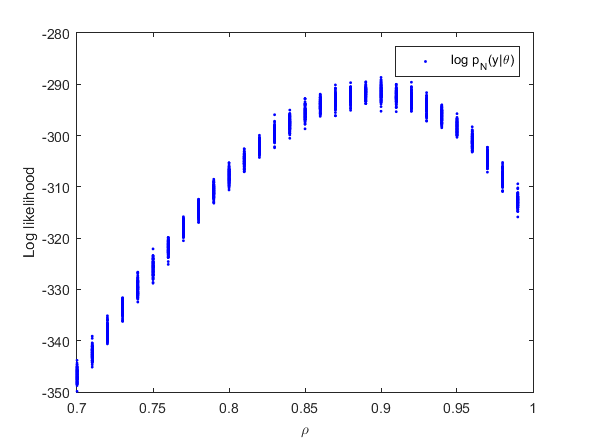
\includegraphics[width=1\textwidth]{tuning_n_rho_varying}
        \caption{$\var(\log \hat{p}_N(y|\theta))$ when $\theta$ varies through $\rho$. Dataset generated from $\mathcal{M}_2$ with $(\rho,\sigma,\nu) = (0.91,1,3)$.}
        \label{tuning_n_rho_varying}
    \end{subfigure}
    \begin{subfigure}[t]{0.46\textwidth}
        \centering
        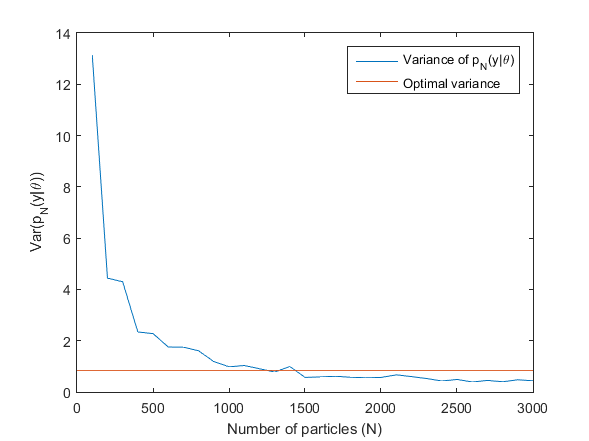
\includegraphics[width=1\textwidth]{tuning_n_optimal_var}
        \caption{$\var(\log \hat{p}_N(y|\bar{\theta}))$ for different values of $N$. Dataset generated from $\mathcal{M}_2$ with $T=1000$ and $(\rho,\sigma,\nu) = (0.91,1,3)$}
        \label{est_var_pn_theta_n}
    \end{subfigure}\\
    \begin{subfigure}[t]{0.46\textwidth}
        \centering
        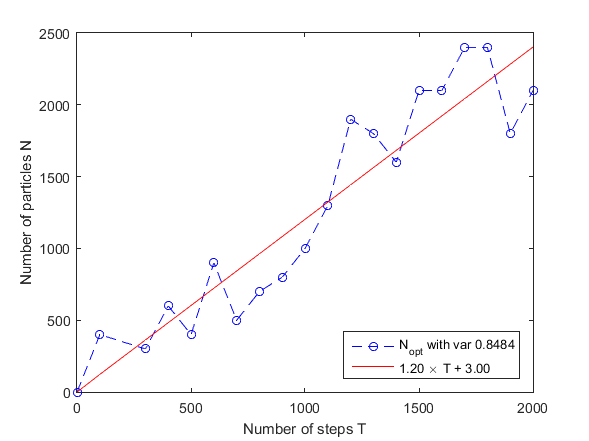
\includegraphics[width=1\textwidth]{n_opt_function_t}
        \caption{Behavior of $N_{opt}$ when $T$ varies}
        \label{n_opt_function_t}
    \end{subfigure}
    \caption{Finding the optimal number of particles $N$}
    %\label{fig:three graphs}
\end{figure}

\chapter{Model Selection and Estimation}

%\section{Validation of the models on Synthetic Data}

In practical applications, the true value of $\theta_{tr}$ is usually unknown and it makes the validation becoming harder. The validation is an important pre-task because it tests the implementation, the choice of the priors and the proposal distributions, and measures the dispersion of the estimator $\hat{\theta}$ to the true value $\theta_{tr}$. The first step involves the sampling generation of both the process and the observations $(X_t, Y_t)$ from a model $\mathcal{M}_x$. We choose an arbitrary realistic value for $\theta_{tr}$. At this point, $x^{tr}_{1:T}$ and $y^{tr}_{1:T}$ are sampled. Each model takes $y^{tr}_{1:T}$ as argument and outputs an estimator $(\hat{x}_{1:T}, \hat{\theta})$. The estimated values are then compared to the true values using some dispersion measures such as the MSE defined by $MSE(\hat{\theta}) = E[ ( \hat{\theta} - \theta_{tr} )^2 ]$. It is also interesting to cross validate the models. The marginal likelihood of the data $p(y^*_{1:T})$ should be maximal for $\mathcal{M}_x$. If the parameters are estimated by another model $\mathcal{M}_y$ say, we should have $p(y^*_{1:T} | \mathcal{M}_x) > p(y^*_{1:T} | \mathcal{M}_y)$ according to the likelihood principles. Each of the 7 models presented in Section \ref{sec:sv} has been successfully validated. The source code of the validation is available in the folder \texttt{models} of the repository (Appendix \ref{app:implementation}).

\section{Parameter Estimation on Real Data}

Once the models have been validated, they can be fitted to real world data. The dataset used here is $\mathcal{EQTY}_{daily}$, presented in \ref{sec:presentation_data}. The number of steps of Particle MCMC is taken large enough to ensure that there is a sufficient number of samples available to form the Bayesian posterior distributions $\mathcal{D}(\theta|y_{1:T})$. Unless stated otherwise, the PMCMC scheme algorithm will loop 10000 times before stopping. The first 1000 samples are discarded for each parameter because the chains require several steps to reach their equilibrium distribution (burn-in). A component-wise scheme is used to update the parameters, i.e. one by one sequentially. Note that it is possible to parallel this scheme by introducing a bias. However, a more efficient way is to parallel the filter, still with a bias. Both algorithms have been implemented and are available in the folder \texttt{pmcmc} (Appendix \ref{app:implementation}). Because the bias has not been rigorously evaluated, a non parallel version was used for the computations throughout the scope of the thesis. Once the burn-in phase is performed, the mean value $\bar{\theta}$ is selected from the distribution $\mathcal{D}(\theta|y_{1:T})$ as the best estimation for $\theta_{tr}$. Some statistics, moments and confidence intervals can be obtained from $\mathcal{D}(\theta|y_{1:T})$. It is also important to choose correctly the prior distributions $p(\theta)$ and the proposal densities $q(\theta|\theta')$ to maintain a good acceptance rate. \cite{roberts1997} showed that the optimal acceptance rate is 0.234 under quite general conditions. \\
Table \ref{est_appl_params} summarizes such an analysis for model $\mathcal{M}_5$ on the stock APPL for the period 2003-Sep-09 - 2006-Jun-04. Figure \ref{sigma_svm_checks} exposes some checks on the posterior distribution $p(\sigma|y_{1:T}, \mathcal{M}_5)$. The chain mixes well with an acceptance rate of 0.180, close to the 0.234 optimal value of \cite{roberts1997}. According to Figures \ref{sigma_svm_2} and \ref{sigma_svm_3}, the posterior distribution seems to be normally distributed, with a skewness of 0.224 and a kurtosis of 2.945. Finally, the autocorrelation function of the chain is fast decaying, which assesses the good performance of the sampling.

\begin{table}[H]
\centering
\begin{tabular}{llll}
Parameter      	& $\rho$ & $\sigma$ & $\beta$ \\ 
\hline
Mean            & 0.9981              & 0.2533             & 0.1475\\
Median          & 0.9982              & 0.2514             & 0.1448\\
Max             & 0.9991              & 0.3941             & 0.2189\\
Min             & 0.9865              & 0.1434             & 0.1100\\
Conf Int (95\%) & [0.9904, 0.9989]    & [0.1822, 0.3345]   & [0.1242, 0.1839]\\
Acceptance Rate & 0.11                & 0.18               & 0.15 \\
MCMC Steps      & 10000               & 10000              & 10000 \\
Burn-in         & 1000                & 1000               & 1000 \\
$p(\theta)$     & $\mathcal{U}[-1,1]$   & $\mathcal{IG}(1,1)$  & $\mathcal{IG}(1,1)$     \\
$q(\theta|\theta')$& $\mathcal{N}(\theta', 0.1^2)$ & $\mathcal{N}(\theta', 0.1^2)$ & $\mathcal{N}(\theta', 0.1^2)$     \\
\hline
\end{tabular}
\caption{Parameters estimation with model $\mathcal{M}_5$. Ticker is APPL. Sep, 09 2003 - Jun, 04 2006.}
\label{est_appl_params}
\end{table}

\begin{figure}[H]
    \centering
    \begin{subfigure}[t]{0.38\textwidth}
        \centering
        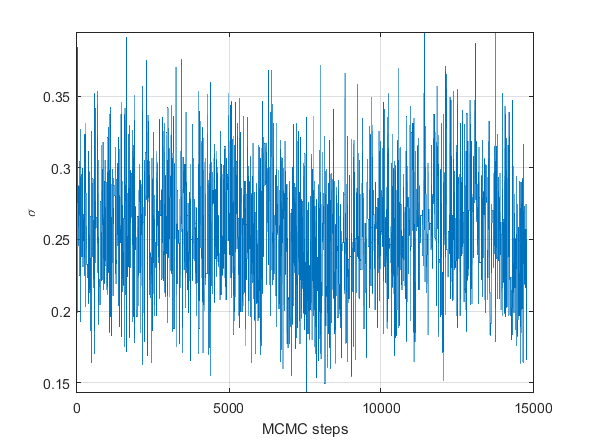
\includegraphics[width=1\textwidth]{sigma_svm/1}
        \caption{MCMC Chain for $\sigma$}
        \label{sigma_svm_1}
    \end{subfigure}
    \begin{subfigure}[t]{0.38\textwidth}
        \centering
        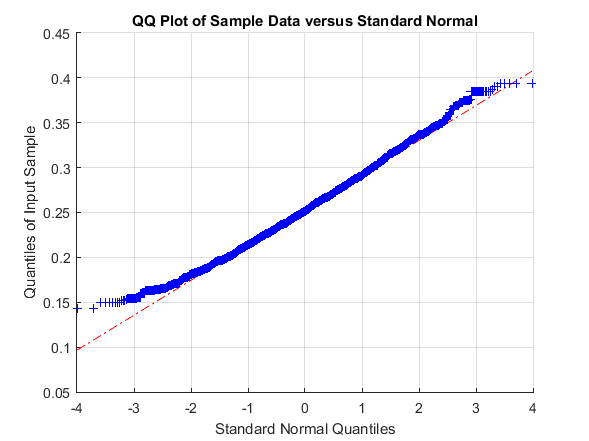
\includegraphics[width=1\textwidth]{sigma_svm/2}
        \caption{QQ Plot - $\sigma$}
        \label{sigma_svm_2}
    \end{subfigure}
    \begin{subfigure}[t]{0.38\textwidth}
        \centering
        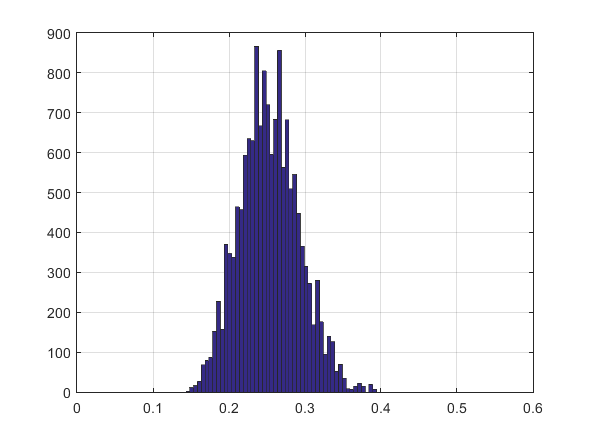
\includegraphics[width=1\textwidth]{sigma_svm/3}
        \caption{Posterior distribution $p(\sigma|y_{1:T})$}
        \label{sigma_svm_3}
    \end{subfigure}
    \begin{subfigure}[t]{0.38\textwidth}
        \centering
        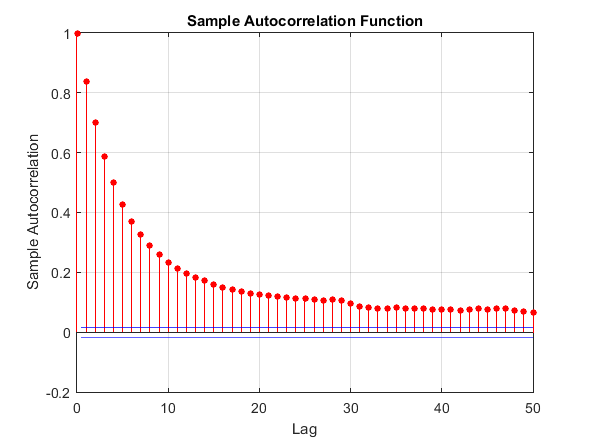
\includegraphics[width=1\textwidth]{sigma_svm/4}
        \caption{Autocorrelation function of $\sigma$}
        \label{sigma_svm_4}
    \end{subfigure}
    \caption{MCMC Checks for $p(\sigma|y_{1:T}, \mathcal{M}_5)$. APPL - Sep, 09 2003 - Jun, 04 2006.}
    \label{sigma_svm_checks}
\end{figure}


\section{Model Selection}
\subsection{Methodology}

The output of the particle filter is an unbiased estimate of $p(y_{1:T}|\theta)$, with the unobserved states integrated out. Although it is very tempting to use it as a measure to compare models, it is always preferred to use the true marginal likelihood $p(y_{1:T})$. According to Bayesian theory, the marginal likelihood for a model $\mathcal{M}$ is defined as

\begin{equation}
p(y_{1:T} | \mathcal{M}) = \int p(y_{1:T} | \theta, \mathcal{M}) p(\theta | \mathcal{M}) d\theta
\end{equation}


\cite{gelfand1994} proposed a very general estimate for this marginal likelihood

\begin{equation}
\left(\frac{1}{M} \sum_{i=1}^M \frac{g(\theta_i)}{p(y_{1:T} | \theta_i) p(\theta_i)}\right)^{-1} \rightarrow p(y_{1:T}) \text{ as } M \rightarrow \infty
\end{equation}
For this estimator to be consistent, $g(\theta_i)$ must be thin-tailed relative to the denominator. \cite{gelfand1994} argued that for most cases, a multivariate normal distribution $\mathcal{N}(\theta^*, \Sigma^*)$ can be used, where $\theta^*$ and $\Sigma^*$ are equal to the empirical mean and sample unbiased variance, $\theta^* = \frac{1}{M} \sum_{i=1}^M \theta^i$ and $\Sigma^* = \frac{1}{M-1} \sum_{i=1}^M \left(\theta^i - \theta^*\right)\left(\theta^i - \theta^*\right)^T$. \\


The difficulty of this approach resides in its implementation. By its definition, $p(y_{1:T} | \theta)$ is usually either very close to 0 or very big as the size of the state-space $T$ grows. The trick here is to consider the sum of the exponential of the logarithms and factorize by the maximum logarithm to avoid rounding errors. For example, let $M = 3$ and assume that the log-terms on the LHS are equal to $-120$, $-121$ and $-122$. Thereby, we have
\begin{align*}
p(Y_T)^{-1} &= e^{-120} + e^{-121} + e^{-122} \\
- \log p(Y_T) &= \log (e^{-120} ( 1 + e^{-1} + e^{-2})) \\
 \log p(Y_T) &= 120 - \log ( 1 + e^{-1} + e^{-2})) \simeq 119.6
\end{align*}

When $p(Y_T | \mathcal{M_A})$ and $p(Y_T | \mathcal{M_B})$ are estimated, \cite{kass1995} suggests to use twice the logarithm of the Bayes factor for model comparison $2 \log BF_{\mathcal{M_{AB}}}$, where $\mathcal{M_{AB}}$ is the Bayes Factor of $\mathcal{M_A}$ to $\mathcal{M_B}$. \textbf{The evidence of $\mathcal{M_A}$ over $\mathcal{M_B}$ is based on a rule-of-thumb: 0 to 2 not worth more than a bare mention, 2 to 6 positive, 6 to 10 strong, and greater than 10 as very strong.}


\subsection{Results}
\label{sec:model_selection}
It is interesting to see how models perform in practical applications. When it seems pretty obvious that using a leverage can be pertinent according to stylized facts, it seems less evident that the mean of the returns exhibits a stochastic mean proportional to its volatility. The best model is selected on a group composed of several cointegrated spreads on different periods. The computationally intensive property makes it difficult to test every model for every spread. A sample of 10 spreads is considered randomly beforehand across different sectors such as Energy, Information Technology and Financial. The conclusion is fairly clear on the random group. It turns out that $\mathcal{M}_7$ outperforms all the other models in every situation, in terms of marginal likelihood and AIC. On average, the Kass Factor of $\mathcal{M}_7$ over $\mathcal{M}_6$ is between 2 and 10, showing a positive evidence. The $\mathcal{M}_2$ and $\mathcal{M}_3$ model are respectively ranked third and fourth. Therefore, model $\mathcal{M}_7$ is selected as the most compelling model for the rest of the analysis. \\

This section also introduces an example with detailed explanations about the procedure we used, for a particular spread and a particular stock. The results are confronted to detect if the inferences are in accordance.
\label{sec:model_selection}
\begin{figure}[H]
    \centering
    \begin{subfigure}[t]{0.49\textwidth}
        \centering
        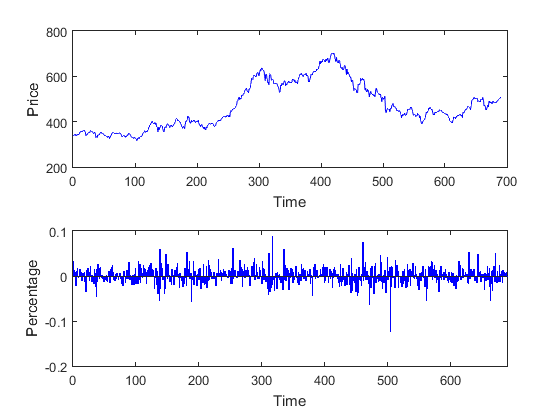
\includegraphics[width=1\textwidth]{apple_2003_2006}
        \caption{APPL stock}
        \label{apple_2003_2006}
    \end{subfigure}
    \begin{subfigure}[t]{0.49\textwidth}
        \centering
        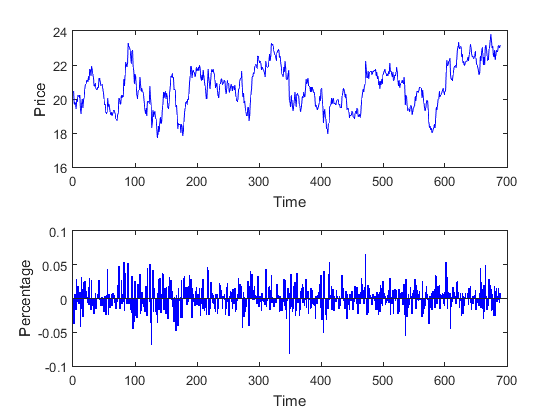
\includegraphics[width=1\textwidth]{spread_amr_crane_2003_2006}
        \caption{Spread AMR CORP - CRANE CO - DOVER CORP. $\beta = (1, -0.0865, -0.3796)$}
        \label{spread_amr_crane_2003_2006}
    \end{subfigure}
    \caption{Stock APPL and Spread AMR-CRANE-DOVER. Period is from 09-Sep-2003 to 04-Jun-2006.}
\end{figure}

The stock at hand is Apple (APPL) on the period Sep, 9 2003 - Jun, 4 2006 (Figure \ref{apple_2003_2006}). The daily returns are computed according to the formula $Y_t = S_t / S_{t-1} - 1$ and are given as input to the stochastic volatility models. We set $N$, the number of particles to 1000 and run the different samplers for $M = 10000$ Metropolis Hastings iterations. After discarding the first 1000 iterations, we collect the final sample and compute the posterior mean $\bar{\theta}$, the posterior median, 95\% credibility intervals, the log likelihoods that results from the particle filter, the logarithm of the marginal likelihood, the AIC criterion and the M-H acceptance ratio. The model with the highest marginal likelihood is taken as reference and the Bayes factors are computed relatively to this model. Table \ref{estimation_of_sv_appl} and \ref{spread_amr_crane_2003_2006} report estimation of $\theta$ for the stochastic volatility models $(\mathcal{M}_1, ..., \mathcal{M}_7)$. $\log (L)$ is the log marginal likelihood $\hat{p}_N(y| \mathcal{M})$. We find that the Gaussian TFSVL model ($\mathcal{M}_7$) performs best in terms of marginal likelihood and AIC criteria. The Kass factor $2 \log BF$ of SVTFL $\mathcal{M}_7$ versus SVTF $\mathcal{M}_6$ is 2.8 which indicates a positive evidence in favor of the SVTF model and its leverage $\rho$. Compared to the SV with leverage $\mathcal{M}_3$ with one factor, the Kass factor in favor of SVL is 10.0 which is a strong evidence. The distribution of the parameters are also fairly concentrated around their means. Overall, the values of $\phi$ are very close to one and confirm strong daily volatility persistence, in accordance to the volatility clustering fact seen in econometrics. The values of $(\phi_X, \sigma_X)$ and $(\phi_Z, \sigma_Z)$ are very interesting. $\phi_X$ is very close to 1 and $\sigma_X$ is small whereas $\phi_Z$ is close to 0 and $\sigma_Z$ is high. It seems clear now that the volatility of the returns can be decomposed into two distinct processes: a long-run stochastic trend $\matr{X}$ and a process $\matr{Z}$ accounting for short-run dynamics. \\

The same procedure was conducted on a spread, composed of three stocks: AMR CORP, CRANE CO and DOVER CORP with associated cointegrating vector $\beta = (1, -0.0865, -0.3796)$. The considered period is the same as the one used for the stock. Table \ref{estimation_of_svm_appl_spr} reports estimation of $\theta$ for the stochastic volatility models $(\mathcal{M}_1, ..., \mathcal{M}_7)$. We find again that the Gaussian TFSVL model ($\mathcal{M}_7$) performs best in terms of the marginal likelihood and AIC criteria. This time, the Kass factor of SVTFL $\mathcal{M}_7$ versus SVTF $\mathcal{M}_6$ is 10.8 which indicates a very strong positive evidence in favor of the SVTF model and its leverage $\rho$. Figure \ref{estimation_of_latent_processes} shows the estimation of the latent processes $\matr{X}$ and $\matr{Z}$ of model $\mathcal{M}_7$ for the spread. 

\begin{figure}[H]
    \centering
    \begin{subfigure}[t]{0.42\textwidth}
        \centering
        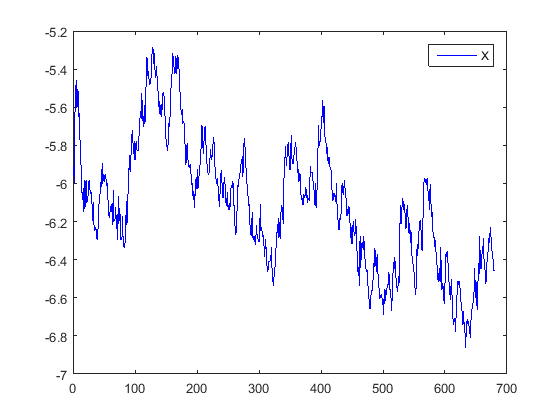
\includegraphics[width=1\textwidth]{est/1}
        \caption{$X_t$}
        \label{est_1}
    \end{subfigure}
    \begin{subfigure}[t]{0.42\textwidth}
        \centering
        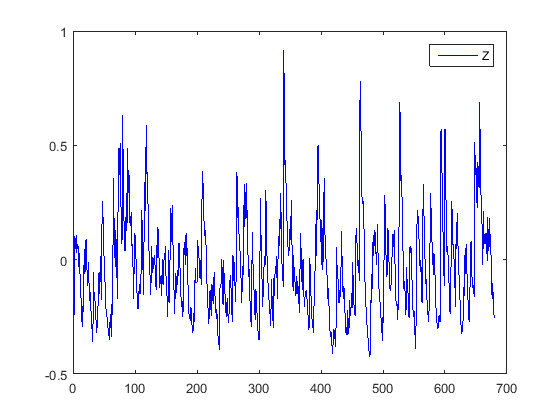
\includegraphics[width=1\textwidth]{est/2}
        \caption{$Z_t$}
        \label{est_2}
    \end{subfigure}
    \caption{Estimation of the latent processes $X_t$ and $Z_t$ of $\mathcal{M}_7$. Data is Spr AMR CORP - CRANE CO - DOVER CORP.}
    \label{estimation_of_latent_processes}
\end{figure}


\begin{table}[H]
\centering
\begin{tabular}{llllllll}
Parameter        & $\bar{\theta}_{\mathcal{M}1}$ & $\bar{\theta}_{\mathcal{M}2}$ & $\bar{\theta}_{\mathcal{M}3}$ & $\bar{\theta}_{\mathcal{M}4}$ & $\bar{\theta}_{\mathcal{M}5}$ & $\bar{\theta}_{\mathcal{M}6}$ & $\bar{\theta}_{\mathcal{M}7}$\\ 
\hline
$\phi$								                  & 0.9991  & 0.9989 & 0.9960  & 0.9981 & 0.9986 & \\
$\sigma$                                & 0.2395  & 0.1983 & 0.2728  & 0.1694 & 0.2533 & \\
$\beta$                                 & 0.8783  & 0.3705 & 0.1     & 0.2359 & 0.1625 & 0.7427 & 0.6992\\
$\nu$                                   &         & 7.6850 &         & & &\\
$\rho$                                  &         &        & -0.4397 & & & & -0.4178\\
$\psi$                                  &         &        &         & 0.0060 & & \\
$\phi_X$                                &         &        &         & & & 0.9995 & 0.9989\\
$\phi_Z$                                &         &        &         & & & 0.3181 & 0.2477\\
$\sigma_X$                              &         &        &         & & & 0.1222 & 0.1906\\
$\sigma_Z$                              &         &        &         & & & 0.6657 & 0.5219\\
$\log(L)$                               & 2646.3  & 2659.7 & 2660.9  & 2649.2 & 2649.3 & 2664.5 & 2665.9\\
AIC                                     & -5286.6 & -5311.4 & -5313.8 & -5290.4 & -5292.6 & -5319.0 & -5319.8\\
$2 \log \mathcal{BF}(\cdot, \mathcal{M}7)$& 33.9  & 12.4    & 10.0     & 33.4  & 33.2 & 2.8 & 0\\
% $N$                                     & 1000    & 1000   & 1000    & 1000  & 1000 & 1000 & 1000\\
% $T$                                     & 1000    & 1000   & 1000    & 1000  & 1000 & 1000 & 1000\\
% Steps                                   & 10000   & 10000  & 10000   & 10000 & 10000 & 10000 & 10000\\
% Burn-in                                 & 1000    & 1000   & 1000    & 1000  & 1000 & 1000 & 1000\\
\hline
\end{tabular}
\caption{Estimation of the SV parameters. Data is APPL.}
\label{estimation_of_sv_appl}
\end{table}

\begin{table}[H]
\centering
\begin{tabular}{llllllll}
Parameter        & $\bar{\theta}_{\mathcal{M}1}$ & $\bar{\theta}_{\mathcal{M}2}$ & $\bar{\theta}_{\mathcal{M}3}$ & $\bar{\theta}_{\mathcal{M}4}$ & $\bar{\theta}_{\mathcal{M}5}$ & $\bar{\theta}_{\mathcal{M}6}$& $\bar{\theta}_{\mathcal{M}7}$\\ 
\hline
$\phi$								                  & 0.9981  & 0.9993 & 0.9986  & 0.9981  & 0.9986 & \\
$\sigma$                                & 0.2238  & 0.1752 & 0.2188  & 0.1694  & 0.2533 & \\
$\beta$                                 & 0.4419  & 0.5722 & 0.4559  & 0.2359  & 0.1625 & 0.3478 & 0.3690\\
$\nu$                                   &         & 7.6850 &         &         &         &\\
$\rho$                                  &         &        & -0.3017 &         &         & & -0.8532\\
$\psi$                                  &         &        &         & 0.0852  &         & \\
$\phi_X$                                &         &        &         &         &         & 0.9995 & 0.9996\\
$\phi_Z$                                &         &        &         &         &         & 0.1926 & 0.7554\\
$\sigma_X$                              &         &        &         &         &         & 0.1268 & 0.0725\\
$\sigma_Z$                              &         &        &         &         &         & 0.4913 & 0.3443\\
$\log(L)$                               & 1792.3  & 1797.8 & 1795.1  & 1793.5  & 1788.5  & 1801.3 & 1806.7\\
AIC                                     & -3578.6 & -3587.6& -3582.2 & -3579.0 & -3571.0 & -3592.6 & -3601.4\\
$2 \log \mathcal{BF}(\cdot, \mathcal{M}7)$& 28.8    & 17.8      & 23.2    & 26.4    & 36.4    & 10.8 & 0 \\
% $N$                                     & 1000    & 1000   & 1000    & 1000    & 1000    & 1000 & 1000\\
% $T$                                     & 689     & 689    & 689     & 689     & 689     & 689 & 689\\
% Steps                                   & 10000   & 10000  & 10000   & 10000   & 10000   & 10000& 10000\\
% Burn-in                                 & 1000    & 1000   & 1000    & 1000    & 1000    & 1000 & 1000\\
\hline
\end{tabular}
\caption{Estimation of the SV parameters. Data is Spr AMR CORP - CRANE CO - DOVER CORP.}
\label{estimation_of_svm_appl_spr}
\end{table}

\section{Estimation of Rolling Volatility of Spread Instruments}
\label{sec:estimation_bollinger_bands_sv}
Once the best Stochastic Volatility model has been selected ($\mathcal{M}_7$ according to Section \ref{sec:model_selection}) and its parameters being estimated, the volatility of the spread can be approximated. The main idea behind using these stochastic volatility models is to catch the dynamics of the spread through a better estimation of its hidden volatility. According to Definition \ref{spread_def}, a spread is a particular linear combination of assets where each asset price is one observation of a more general process, over a time interval. For a given first order Markov $n$-process $\matr{X}_t$, the returns $y_{1:T}$ modelled by a SV model, are usually of the form $y_t | \matr{x}_t, \theta \sim \mathcal{D} \left( \mu_\theta(t), \sigma_\theta^2(t) \right)$, where $\mathcal{D}$ can represent any suitable distribution in a location-scale family (Definition \ref{location_scale_family}). By definition, $Y_t = S_t / S_{t-1} - 1$. We then have
\begin{equation}
S_t | S_{t-1}, \matr{x}_t, \theta \sim \mathcal{D} \left(S_{t-1} \mu_\theta(t)+S_{t-1}, |S_{t-1}|^2 \sigma_\theta^2(t) \right) \numberthis \label{equation_price_vol}
\end{equation}
where the volatility $\sigma_\theta^2(t)$ and the mean $\mu_\theta(t)$ are known quantities because they depend on $\mathcal{F}_{t-1}$-measurable quantities. \\

In order to estimate the rolling volatility of the spread $S_t$, we generate many Monte Carlo paths according to Equation (\ref{equation_price_vol}). Algorithm \ref{rolling_volatility_algo} explains the procedure when model $\mathcal{M}_7$ (TFSVL) is considered\footnote{The volatility computed in this approach is of the same shape as the one computed in the default Bollinger bands (Equation \ref{bolls_computations}).}. In the most general case, $M$ paths $\{S_{t,n}\}_{0 < n \leq M, t \in \mathbb{N}^*}$ are generated from Equation (\ref{equation_price_vol}). Let $f_a : \mathbb{R}^{+M} \rightarrow \mathbb{R}^+$ be a positive-definite aggregating function. The aggregated rolling volatility of lag $p$ for all the $M$ paths is defined as $r\sigma_p(t) = f_a(r\sigma_p(t)_1,...,r\sigma_p(t)_M)$ for $t >0$. If $f_a$ is simply the sample mean estimator, the equation is simplified to $r\sigma_p(t) = \frac{1}{M}\sum_{i=1}^M r\sigma_p(t)_i$. Depending on the context, $f_a$ can be any measurable function satisfying the conditions above. Throughout the scope of this thesis, $f_a$ will be equal to the sample mean. Without any more information, the sample mean is a pertinent measure to summarize a set of points in one single point.

\begin{algorithm}
\caption{Rolling volatility computation for model $\mathcal{M}_7$ (TFSVL)}
\label{rolling_volatility_algo}
\begin{algorithmic}[1]
\Procedure{RollingVolatility}{$x_{1:T}, z_{1:T}, S_{1:T}$, $\theta = \beta$, $M$, $f_a = M^{-1} \sum_{i=1}^M \cdot$, $p$}

\For{t from 1 to T}
	\For{i from 1 to M}
		\State Sample the $t^{th}$ value of the $i^{th}$ path, $S_{ti} \sim \mathcal{M}(S_{t-1}, S_{t-1}^2 \beta^2 \exp(x_t + z_t))$
	\EndFor{end}
\EndFor{end}
\For{i from 1 to M}
	\State Compute the default rolling volatility $(r\sigma_p(t)_i)_{t>0}$ for the $i^{th}$ path, $(S_{ti})_{t>0}$
\EndFor{end}

\For{t from 1 to T}
	\State $\displaystyle{r\sigma_p(t) = M^{-1} \sum_{i=1}^M r\sigma_p(t)_i}$
\EndFor{end}
\\
\Return $r\sigma_p(t)$
\EndProcedure
\end{algorithmic}
\end{algorithm}

\chapter{Statistical Arbitrage Strategies}
Statistical arbitrage conjectures statistical mis-pricings or price relationships that are true in expectation, in the long run when repeating a trading strategy. It describes a variety of automated trading systems which commonly make use of data mining, statistical methods and artificial intelligence techniques. A popular strategy is pairs trade, in which stocks are put into pairs by fundamental or market-based similarities. When one stock in a pair outperforms the other, the poorer performing stock is bought (long) with the expectation that it will climb towards its outperforming partner, and the other is sold (short). This approach has the advantage of eliminating the market exposure. The idea can be easily generalized to $n$ stocks or assets where an asset can be a sector index. The investment strategy we aim at implementing is market neutral, thus we will hold a long and a short position both having approximately the same value in local currency. It is important to understand that the quantity to interest is the pseudo difference between the assets, better known as the spread. The approach abstracts the trading on the underlying assets and primarily focuses on spread trading. The common strategy is to evaluate if the spread instrument is either underpriced or overpriced. A typical way is to open a position once the spread deviates far from its long-run equilibrium, and unwind it when it reverts. Dealing with spreads instead of non-stationary assets is beneficial because stationary series are on average more reverting due to their nature. \\

In this section, two main strategies are presented: Bollinger bands and Z-score. The first one models a time-varying mean for the spread and time-varying volatility bands (with simple or complex modelling) to gauge the spread deviation, whereas the second one assumes a fixed non-zero mean and fixed volatility bands.

\section{Bollinger Bands}
\label{sec:bollinger_bands}

Bollinger bands is a widely used technical volatility indicator invented by John Bollinger in the 1970s which consists of using a moving average $m_\theta(t)$ of lag $p$ with two volatility bands $B_\theta^+(t), B_\theta^-(t)$, above and below it. The computation of the volatility bands involves a windowed standard deviation of lag $p$ (Definition \ref{windowed_volatility}). The shift between the bands and the stochastic mean is proportional to a parameter called $\alpha$. The bands will expand and contract as the prices become volatile or bound into a tight trading pattern. When prices continually touch the upper bound $B_\theta^+(t)$, the spread is considered to be overbought. Conversely, when they continually touch the lower band, it is oversold. The indicator is calculated by
\begin{align*}
m_{SMA}(t,p) &= \frac{1}{p}\sum_{j=1}^p S_{t-j} \numberthis \label{bb_m} \\
m_{EMA}(t,p) &= k \times S_t + (1-k) \times m_{EMA}(t-1,p) \text{, } k = 2/(p+1) \numberthis \label{bb_ema} \\
B^\pm(t,p,\alpha) &= m(t,p) \pm \alpha \underbrace{\sqrt{\frac{1}{p} \sum_{j=1}^p \left(S_{t-j} - m(t,p) \right)^2}}_{r\sigma_B(t,p)} \numberthis \label{bolls_computations}
\end{align*}
where $S_t$ is the price of the spread, $p$ is the lag and $\alpha$ is the number of standard deviations to shift the Bollinger bands. According to John Bollinger, the default values are $p = 20$ and $\alpha = 2$. $m_\theta(t)$ is the mid band used as a relative mean value. The exponential moving average (EMA) gives more weights to new values and may be faster to detect opportunities. $B^+_\theta(t)$ and $B^-_\theta(t)$ are respectively the upper and lower bands. Their intrinsic purpose is to measure how far the price deviates from its mean. Under the mild assumption that the returns are normally distributed and independent, approximately 95\% of the prices should appear within the bands when $\alpha = 2$. Figures \ref{bollinger_bands_intro} and \ref{bollinger_bands_intro_2} show different configurations of the Bollinger bands applied to Walt Disney Co NYSE for the year 2002, all computed with Equations (\ref{bb_m}), (\ref{bb_ema}) and (\ref{bolls_computations}).

\begin{figure}[H]
    \centering
    \begin{subfigure}[t]{0.49\textwidth}
        \centering
        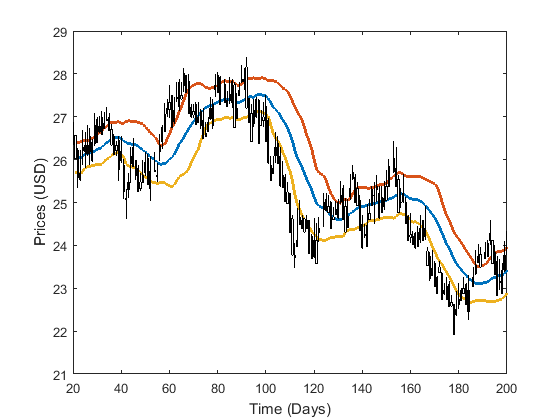
\includegraphics[width=1\textwidth]{bollinger/1}
        \caption{$(p, \alpha, t) = (20,1.0, SMA)$}
        \label{bollinger1}
    \end{subfigure}
    \begin{subfigure}[t]{0.49\textwidth}
        \centering
        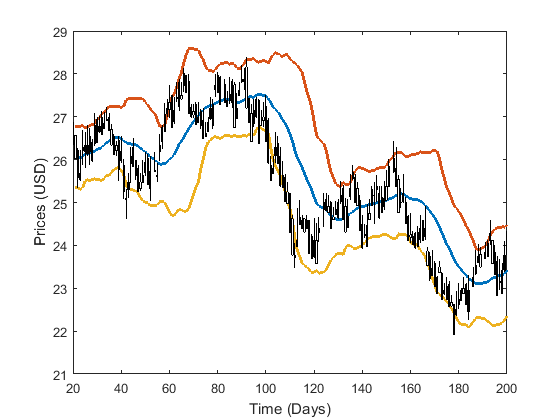
\includegraphics[width=1\textwidth]{bollinger/2}
        \caption{$(p, \alpha, t) = (20,2.0, SMA)$}
        \label{bollinger2}
    \end{subfigure}
    \caption{Simple Bollinger bands strategy applied to Walt Disney Co NYSE for the year 2002. Lag is 20 days. $B^+_\theta$ is red, $B^-_\theta$ yellow and $m_\theta$ Navy blue.}
    \label{bollinger_bands_intro}
\end{figure}

\begin{figure}[H]
    \centering
    \begin{subfigure}[t]{0.49\textwidth}
        \centering
        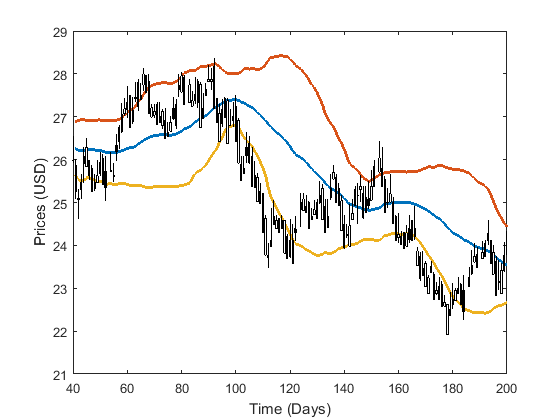
\includegraphics[width=1\textwidth]{bollinger/3}
        \caption{$(p, \alpha, t) = (40,1.5, SMA)$}
        \label{bollinger3}
    \end{subfigure}
    \begin{subfigure}[t]{0.49\textwidth}
        \centering
        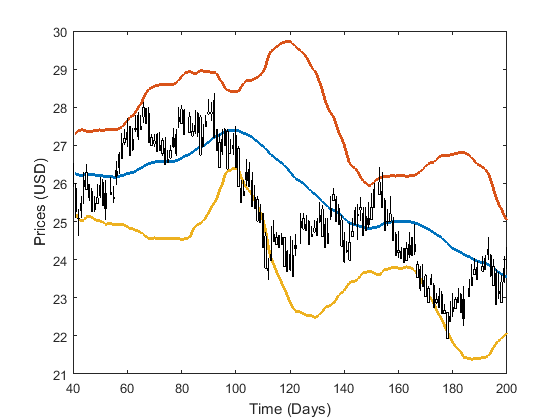
\includegraphics[width=1\textwidth]{bollinger/4}
        \caption{$(p, \alpha, t) = (40,2.5, SMA)$}
        \label{bollinger4}
    \end{subfigure}
    \caption{Simple Bollinger bands strategy applied to Walt Disney Co NYSE for the year 2002. Lag is 40 days. $B^+_\theta$ is red, $B^-_\theta$ yellow and $m_\theta$ navy blue.}
    \label{bollinger_bands_intro_2}
\end{figure}

A trading rule determines the correct timing when to open and close a position. With the Bollinger bands strategy, the rule is

\begin{itemize}
\item LONG - Open a long position when there is an upward crossing between the spread and the lower band. Unwind this position when there is an upward crossing between the spread and the upper band;
\item SHORT - Open a short position when there is a downward crossing between the spread and the upper band; Unwind this position when there is a downward crossing between the spread and the lower band.
\end{itemize}

\section{Z-score}
Z-score is a strategy based on mean-reverting patterns but unlike the Bollinger bands, Z-score assumes a non-zero constant mean and constant volatility bands. For this reason, Z-score is only suitable for stationary processes such as spread instruments. Z-score is a dimensionless indicator defined as $z_t = (S_t-\mu_S) / \sigma_S$, where $\mu_S$ and $\sigma_S$ are respectively the unconditional mean and variance of the spread. $z_t$ measures the distance to the long-term mean in units of long-term standard deviation. The basic rule is to open/close a position when the Z-score hits a predefined $n$-quantile of the standard normal distribution $\Phi^{-1}(q_n)$. If the Z-score hits a low threshold, it means that the spread is underpriced and a long position should be opened. When the spread reverts to its mean, the position is unwound. A same reasoning is done for short positions. \cite{caldeira2013} suggested the basic trading strategy signals: Open long position if $z_t \leq \Phi^{-1}(q_{OL}) = -2.00$, open short position if $z_t \geq \Phi^{-1}(q_{OS}) = 2.00$, close short position if $z_t \leq \Phi^{-1}(q_{CS}) = 0.75$ and close long position if $z_t \geq \Phi^{-1}(q_{CL}) = -0.50$. Figure \ref{zscore_graphical_strat} shows the spread $S_t$, the Z-score $z_t$ and the thresholds $\Phi^{-1}(q)$ of the strategy.


\begin{figure}[H]
\centering
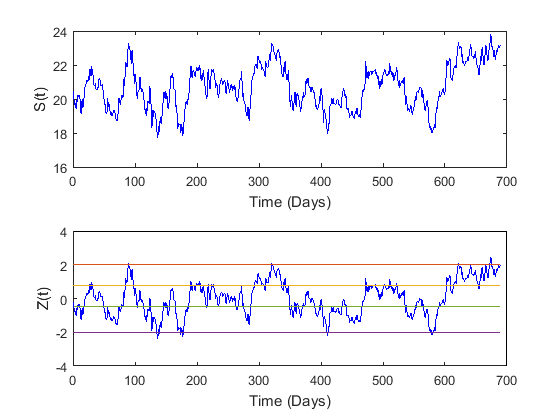
\includegraphics[width = 0.75\textwidth]{zscore/zscore1}
\caption{Spread $S_t$ (defined in Section \ref{sec:model_selection}) and its Z-score $z_t$. From top to bottom: $\Phi^{-1}(q_{OS}), \Phi^{-1}(q_{CS}), \Phi^{-1}(q_{CL}), \Phi^{-1}(q_{OL})$.}
\label{zscore_graphical_strat}
\end{figure}

Unlike the Bollinger bands, the Z-score is highly sensitive to stochastic trends because the mean is assumed to be strictly constant. In other words, it could be dangerous if the spread lost its cointegrated property and became divergent. In practical applications and according to the risk policy, a stop loss threshold is usually set to avoid any huge losses.

\section{Selection of the Cointegrated Tuples}
The assumption that the pairs should belong to the same sector is very common in the literature. Some examples include \cite{chan2009} and \cite{dunis2010}. Other such as \cite{caldeira2013}, did not adopt this restriction but bound their study to pairs trading applied to the Brazilian markets. 

\subsection{Complexity Reduction with Correlation}
\label{Complexity_Reduction_with_Correlation}
In the general case and according to \cite{vidyamurthy2004}, cointegration implies correlation but the reverse is not true. Spurious regression is a very good example where the reverse is not true. The idea is to filter the uncorrelated tuples to limit the number of candidates for cointegration testing. This assertion holds because a cointegration test is more time-consuming than a correlation test (Table \ref{time_spent_test_bivariate}).

\begin{table}[H]
\centering
\begin{tabular}{llllll}
\hline
\multicolumn{1}{|l|}{Test}     & \multicolumn{1}{|l|}{Min} & \multicolumn{1}{|l|}{Max} & \multicolumn{1}{|l|}{Avg} & \multicolumn{1}{|l|}{Std} & \multicolumn{1}{|l|}{95\% Conf. Int.} \\ \hline
Correlation $corr$						 &  0.26  & 1.00  & 0.33  & 0.10 & [0.26 , 0.70]\\
Correlation $R^2$ (fast)       &  0.47  & 1.45  & 0.58  & 0.18 & [0.48 , 1.19]\\
Johansen                       &  16.77 & 37.96 & 19.23 & 3.74 & [16.93 , 34.04]\\
Aug. Dickey Fuller             &  1.68  & 3.42  & 1.96  & 0.33 & [1.68 , 3.31]\\
Phillips-Perron                &  2.62  & 5.93  & 2.99  & 0.67 & [2.63 , 5.66]\\
\hline
\end{tabular}
\caption{Average time spent to test a bivariate time series $\matr{X}_t$ (in milliseconds)}
\label{time_spent_test_bivariate}
\end{table}

When it comes to pairs trading, a simple correlation test is enough. When $n \geq 3$, it is preferred to use the multiple correlation coefficient, better known as $R^2$. It can be computed using the vector $c = (r_{\matr{x}_1\matr{y}}, r_{\matr{x}_2\matr{y}},...,r_{\matr{x}_N\matr{y}})^T$ of correlation $r_{\matr{x}_n\matr{y}}$ between the predictor variables $(\matr{x}_n)_{1 \leq n \leq N}$ and the target variable $\matr{y}$. The correlation matrix $R_{\matr{x}\matr{x}}$ of inter-correlations (Equation \ref{rxx}) between predictor variables also comes into play. It is given by $R^2 = c^T R_{\matr{x}\matr{x}}^{-1}c$.

\begin{equation}
R_{\matr{x}\matr{x}} =\begin{pmatrix}
r_{\matr{x}_1\matr{x}_1}    & r_{\matr{x}_1\matr{x}_2} & ...  & r_{\matr{x}_1\matr{x}n}  \\
r_{\matr{x}_2\matr{x}_1}    & \ddots &   & \vdots  \\
\vdots       &   & \ddots &   \\
r_{\matr{x}_n\matr{x}_1}    & \hdots &   & r_{\matr{x}_n\matr{x}_n} \label{rxx} \\
\end{pmatrix} 
\end{equation}
It is worth noting that $R^2$ is order-dependent. To provide convincing evidence of this fact, let us consider a simple example. A regression of $\matr{y}$ on $\matr{x}$ and $\matr{z}$ will in general have a different $R^2$ that will a regression of $\matr{z}$ on $\matr{x}$ and $\matr{y}$. Let $\matr{z}$ be uncorrelated with both $\matr{x}$ and $\matr{y}$ while $\matr{x}$ and $\matr{y}$ are linearly related to each other. A regression of $\matr{z}$ on $\matr{y}$ and $\matr{x}$ will yield a $R^2$ of zero, while a regression of $\matr{y}$ on $\matr{x}$ and $\matr{z}$ will yield a strictly positive $R^2$. It means that the ordering inside a tuple has its importance at least from a statistical point of view, as highlighted in Definition \ref{definition_tuple}. This assertion is also true for most cointegrations tests. This notion of ordering is however less obvious from a pure financial point of view. \\

An example is presented with $n=4$ in Appendix \ref{sec:corr_analysis_quad}. In this case, the assumption of the same sector is almost inevitable. It becomes interesting to question it for triples trading, which is the purpose of the next section.

\subsection{Sector Analysis for Triple Trading}
\cite{chan2009} and \cite{dunis2010} argued that the pairs should belong to the same sector, otherwise the cointegration and the correlation would be purely fortuitous. To check the veracity of this assumption for triple trading, all the possible cointegrated triples ($n$ = 3) are formed on the whole period of the dataset  - from January, 01 1990 to March, 14 2014 - and the $R^2$ is computed using the methodology exposed in Section \ref{Complexity_Reduction_with_Correlation}. The cointegrated triples are then sorted according to their $R^2$ from the highest to the lowest value. Each triple is characterized by the sector criteria: \textit{All}, \textit{Partial} or \textit{None}. \textit{All} means the three assets composing the triple belong to the same sector, \textit{Partial} that exactly two belong to the same sector, \textit{None} that no one belongs to the same sector. As a result, 30418 cointegrated triples were formed. 816 belonged to \textit{All}, 10517 to \textit{Partial} and the remaining 19085 to \textit{None}. Figure \ref{triples_sector_1} shows that for very high $R^2$ on daily returns, almost all the cointegrated triples belong to the same sector. Then for high $R^2$, the proportion of partial triples becomes higher than two other groups until the half of the set. The conclusion is that when the number of selected cointegrating triples is not very large (less than 500 or 1.5\% here for the whole period), it might be reasonable to consider the assumption of the same sector for increased execution speed. However, the same sector approach will only be retained for quadruples trading and not for triple trading because the computational cost is still affordable.

\begin{figure}[H]
    \centering
    \begin{subfigure}[t]{0.46\textwidth}
        \centering
        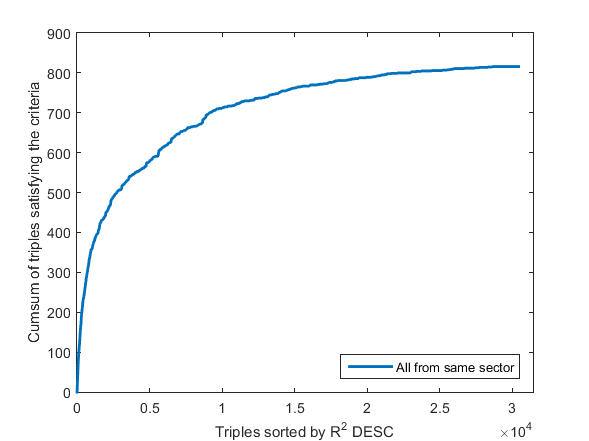
\includegraphics[width=1\textwidth]{triples_sector_0}
        \caption{Cumulative sum of the cointegrated triples from the same sector sorted by $R^2$ from highest to lowest.}
        \label{triples_sector_0}
    \end{subfigure}
    \begin{subfigure}[t]{0.46\textwidth}
        \centering
        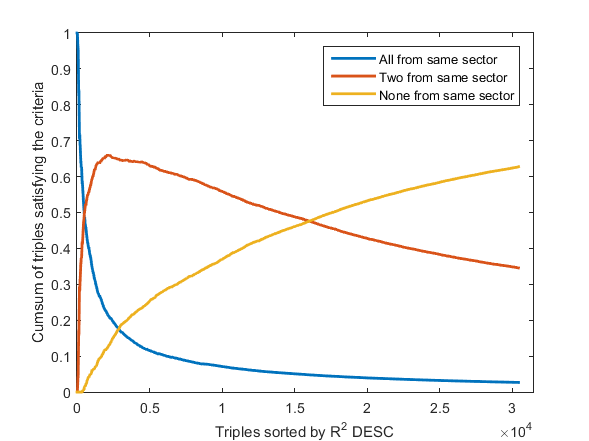
\includegraphics[width=1\textwidth]{triples_sector_1}
        \caption{Distribution of the cointegrated triples sorted by $R^2$ from highest to lowest and regarding their belonging to sectors.}
        \label{triples_sector_1}
    \end{subfigure}
    \caption{Distributions of the cointegrated triples. Period is Jan, 01 1990 - Mar, 14 2014.}
\end{figure}

\chapter{Procedure}
The workflow involves the preparation of the datasets and the selection of the cointegrated tuples. Then, the three strategies $\mathcal{B}_{STD}$, $\mathcal{B}_{SV}$ and $\mathcal{Z}$ are applied and backtested on the data. Finally, the cumulative returns and some risk measures are presented to assess the performance of the strategies.

\section{General Framework}

\subsection{Training and Simulation Sets}
We use the dataset $\mathcal{EQTY}_{daily}$ defined in Section \ref{sec:presentation_data}. The whole sample period is divided sequentially into sets of length \textbf{two} years. Each set is split into two sets: the in-sample set denoted $\mathcal{I}$ followed by the out-of-sample $\mathcal{O}$ with a 1:2 ratio: $(\mathcal{I}_i, \mathcal{O}_i)_{1 \leq i \leq 12}$. Roughly, each training set has 169 trading days and each testing set 336 days. The idea is to backtest the strategies with a rolling time window scheme. The asymmetric choice of the ratio is motivated by the fact that the Bollinger bands has a stochastic mean and are therefore less sensitive to a break of the cointegration property, contrary to the Z-score which is only considered as a benchmark. Detection of cointegrated tuples, selection of the best tuples or tuning of the Bollinger bands parameters $(p,t,\alpha)$ is done on $\mathcal{I}$. The purpose of $\mathcal{O}$ is to assess the performance of the strategy on unseen data with the parameters computed in the training period. This technique is known as cross validation and is used to avoid overfitting during the calibration. 


\subsection{Framework Hypotheses}

Only two types of transactions are considered: move into a new position and unwind a previously opened position. The operations on the spread are assumed to be atomic, i.e., they have a succeed-or-fail property. At the end of each trading period, all the outstanding positions are closed. When a long position is initiated, the first asset is bought with quantity 1 and the remaining assets of the tuple are sold with the respective quantities indicated by the cointegrating vector $\beta$. This same position is closed by selling one unit of the first asset and buying the remaining assets, still in the same proportions. It is assumed that the trader can buy a portion of an asset. For any spread instrument, the number of simultaneously opened positions is limited to two: one long and one short. We consider 5 point basis of transaction costs. This choice was made for pairs trading in \cite{dunis2010}, \cite{dunis2005} and \cite{alexander2002}. For simplicity, no stop loss policy or rental costs are considered but the capital invested in short selling cannot exceed half of the total capital, either invested or in cash. The initial cash balance of any simulation is 10000 USD.

\subsection{HRSRI Portfolio Approach}

The HRSRI (Highest-Ranked Sharpe Ratios on $\mathcal{I}$) portfolio approach consists in ranking the cointegrated tuples based on the best in-sample Sharpe ratios $\mathcal{SR}$ for every period training-testing. For each period, the 20 highest-ranked tuples are used to compose the portfolio. The first motivation of considering a portfolio is to lower the volatility associated to each tuple trading by smoothing the net value over time. The asset allocation in the portfolio follows an investing weighting scheme with no dynamic rebalancing. At each time, the portfolio valuation is a linear combination of each valuation, where the weights are constant and equally distributed. \\

An example is provided with a portfolio composed of two spread instruments: $S_1$ and $S_2$. Denote their respective cumulative returns by $CR_{S_1}(t)$ and $CR_{S_2}(t)$. At each time, the valuation of the portfolio is simply given by $p(t) = 0.5 \times CR_{S_1}(t) + 0.5 \times CR_{S_2}(t)$ where the weights (0.5,0.5) will remain constant once the portfolio is created. Each $S_1$ and $S_2$ is strictly allocated $10000/2 = 5000$ USD, resulting in no money re-allocations between the instruments. Note that a portfolio is always composed of 20 triples selected from a cross validation phase. As a triple is itself composed of 3 stocks, the maximum number of stocks to monitor is 60 for a single portfolio. 

\section{Optimization of the Strategies}
\label{sec:optimization_strategy}
The optimization of the Bollinger bands strategy requires to tune three parameters: the number of periods $p$ to compute the bands, the type $t$ of moving average (EMA or SMA) used in the mid band and $\alpha$ which controls the interval between the volatility bands. John Bollinger suggests $p = 20, \alpha = 2$ and exponential moving average as default values. To get the best out of the strategy, a cross validation is performed on the in-sample set $\mathcal{I}$. The criterion of optimization is the in-sample Sharpe ratio $\mathcal{SR}$. The cross validation parameter space is denoted  $\Omega_{CV} = \mathcal{P}_n \times \mathcal{P}_t \times \mathcal{P}_\alpha$. An exhaustive search is made possible because of the efforts invested into the parallelization of the task. This search provides good visual results and is therefore our recommended choice to reveal the topology of $f(\Omega_{CV}) \rightarrow \mathbb{R}$. The dataset is split into two sets $\mathcal{I}$ and $\mathcal{O}$ with a ratio 2:1. \\

In practical applications, the parameter space is defined as $\Omega_{CV}  = [5,6,...,200] \times \{\text{SMA}, $\\$\text{EMA}\} \times [1,1.1,...,2.9,3.0]$ and the function $f(\Omega_{CV}) \rightarrow \mathbb{R}$ outputs a Sharpe ratio surface (Definition \ref{sharpe_ratio_def}). The idea is to find regions, not peaks where $f$ has a stable global maximum. As $f$ is multivariate, the idea is to detect a region where $\nabla F(\rho_{max}, \sigma_{max}, t_{max}) = 0$ where the gradient $\nabla F$ is defined on a 3D space $(\vec{i}, \vec{j}, \vec{k})$ by
\begin{equation}
\nabla F = \frac{\partial F}{\partial \rho} \vec{i} + \frac{\partial F}{\partial \alpha} \vec{j} + \frac{\partial F}{\partial t} \vec{k}
\end{equation}
In a metric space, $M = (\Omega, d)$, a Borel $\sigma$-algebra $\mathcal{V} = \mathcal{B}(\Omega)$ is a region of a point $p$ if there exists an open ball with center $p$ and radius $r > 0$, such that $B_r(p) = \{\omega \in \Omega | d(\omega, p) < r\}$ is contained in $\mathcal{V}$. To find a suitable global maximum, an exhaustive search is performed for every $\omega \in \Omega$ for $r$ fixed. Then, the Sharpe ratios are sorted in the descending order $sr_1 > sr_2 > ... > sr_{card(\Omega)}$. The highest Sharpe ratio $sr_1$ is considered and its region evaluated with a suitable $r$. The gradient is then evaluated and checked if it is close to 0. If this is the case, $(p_1, \alpha_1, t_1, sr_1)$ is selected. If not, $sr_1$ is dropped and $sr_2$ is now considered. The procedure goes on until a Sharpe ratio is selected.
 
\section{Performance Assessment}
Once the strategy ran on $\mathcal{I}$, it can be assessed on the out-sample set $\mathcal{O}$. The performance of the portfolios are examined in terms of cumulative return (CR), Sharpe ratio (SR) and Maximum Drawdown (MDD). \\

Let $y_t$ denote the simple daily return on a particular asset at time $t$. 

\subsection{Maximum Drawdown}
The maximum drawdown (MDD) is defined as the maximum percentage drop incurred from a peak to a bottom up to time $T$. It is the worst possible scenario up to time $T$. By construction, it is higher in absolute values than the maximum loss. Indeed, this is the most pessimistic scenario. Figure \ref{mdd} provides a graphical interpretation of the Maximum Drawdown.

\begin{equation}
MDD(T) = \smash{\displaystyle\max_{s \in (0,T)}} \left[\smash{\displaystyle\max_{s \in (0,T)}} y_t - y_s \right] 
\end{equation}

\begin{figure}[H]
\centering
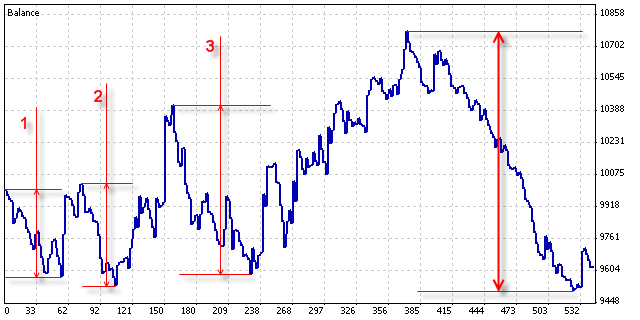
\includegraphics[width = 0.8\textwidth]{mdd}
\caption{Evolution of the Maximum Drawdown for a synthetic portfolio}
\label{mdd}
\end{figure}

\subsection{Sharpe Ratio}
The Sharpe ratio ($\mathcal{SR}$) based on daily returns is defined as
\begin{equation}
\mathcal{SR} =  \frac{\hat{\mu}}{\hat{\sigma}} \text{ where, } \hat{\mu} =  252  \times \frac{1}{T} \sum_{t=1}^T y_t \text{ and } \hat{\sigma} = \sqrt{252} \times \frac{1}{T} \sum_{t=1}^T (y_t - \bar{\mu})^2 \label{sharpe_ratio_def}
\end{equation}
$\hat{\mu}$ represents the mean asset return and $\hat{\sigma}$ the standard deviation of the returns. According to the NYSE, there is about 252 trading days on average per year. The idea of the Sharpe ratio is to quantify how much additional return the investor is receiving for the additional volatility of holding the risky asset over a risk-free asset. A variant is to subtract the daily risk free return $y_{rf}$, given by the US Treasury bills, to the returns of the strategy. This version is expected to output a slightly lower but more accurate value. \textbf{A general rule of thumb is: a ratio of 1 or better is considered good, 2 and better is very good, and 3 and better is considered excellent.} \\

\subsection{Buy and Hold Strategy}
Finally, one technique to assess the performance of a strategy is to compare it to the standard Buy and Hold (B\&H) strategy where the holder has a portfolio replicating the stock index from time 0 to $T$.

\chapter{Empirical Analysis on Triple Trading}
This chapter is focused on triple trading and is structured in four main parts. Firstly, a case study is examined to show some interesting facts about volatility modelling. Then, the three strategies are backtested on the Equity dataset and are compared to the SPX Buy and Hold strategy. On top of this, an exhaustive comparison between the two Bollinger bands is performed to evaluate whether using more advanced modelling will result to better performance than simple models used often in practice. Finally, parameters tuning is attempting to improve profitability. The aim is to assess  


\section{Volatility Modelling of Spread Instruments with $\mathcal{M}_7$}
Throughout this section, the same spread $S_t$ as that of Section \ref{sec:model_selection} is considered. This procedure is not restricted to this particular spread and is valid for any stationary spread and any stochastic volatility models. This section focused on the main points described in Section \ref{sec:estimation_bollinger_bands_sv}. The model $\mathcal{M}_7$ is used to estimate the conditional variance $S_t | S_{t-1}, \matr{x}_t, \theta$. From there and from Equation (\ref{equation_price_vol}), $M = 1000$ Monte Carlo trajectories are generated. Figure \ref{fig:generation_of_the_trajectories} shows the generation of the trajectories according to the estimated conditional variance.
\begin{figure}[H]
    \centering
    \begin{subfigure}[t]{0.49\textwidth}
        \centering
        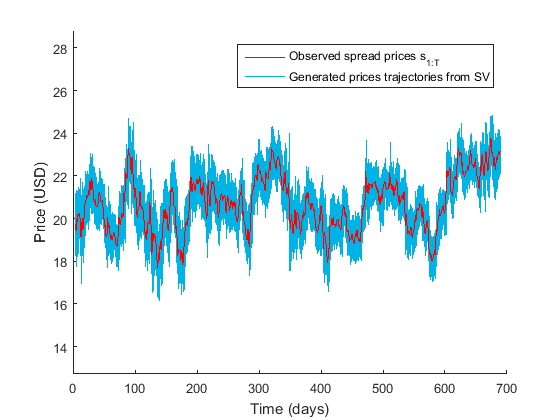
\includegraphics[width=1\textwidth]{model_vol/1}
        \caption{Generation of $M = 1000$ MC prices trajectories with model $\mathcal{M}_7$}
        \label{vol_mod_1}
    \end{subfigure}
    \begin{subfigure}[t]{0.49\textwidth}
        \centering
        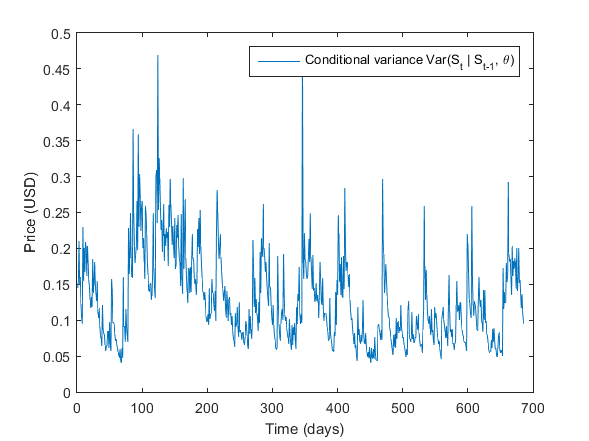
\includegraphics[width=1\textwidth]{model_vol/2}
        \caption{Conditional variance of $S_t | S_{t-1}, \matr{x}_t, \theta$ with model $\mathcal{M}_7$}
        \label{vol_mod_2}
    \end{subfigure}
    \caption{Generation of the trajectories of the spread process $S_t$}
    \label{fig:generation_of_the_trajectories}
\end{figure}

The next step is to compute the rolling volatility for every trajectory. The aggregated function $f_a$ is the sample mean and $r\sigma_{SV}(t)$ is the resulting aggregation of the MC trajectories. The standard rolling volatility on the observed prices $s_{1:T}$ is denoted $r\sigma_{STD}(t)$. Then, 90\% and 95\% confidence intervals are derived for every $t \in [1,T]$ using Monte Carlo. The results are presented in Figure \ref{fig:rolling_vol_and_confidence_intervals}\footnote{It is worth noting that the time axis has been truncated to improve readability. The analysis and the conclusions are carried and made on the whole period $[1,T]$.}. It turns out that $r\sigma_{STD}(t)$ is clearly underestimated most of the time. Only 63.9\% of $r\sigma_{STD}(t)$ is contained inside the 0.90 confidence intervals and 78.3\% inside the 0.95 confidence intervals. Moreover, Figure \ref{fig:diff_vol} summarizes the difference $\delta(t) = r\sigma_{SV}(t) - r\sigma_{STD}(t)$. With $E[\delta] = 0.1035$ (USD), the standard volatility estimator is clearly biased.
\begin{figure}[H]
    \centering
    \begin{subfigure}[t]{0.49\textwidth}
        \centering
        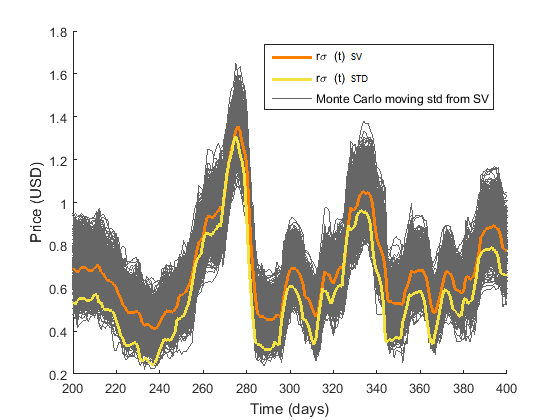
\includegraphics[width=1\textwidth]{model_vol/3}
        \caption{Generated prices trajectories with rolling volatility processes}
        \label{vol_mod_3}
    \end{subfigure}
    \begin{subfigure}[t]{0.49\textwidth}
        \centering
        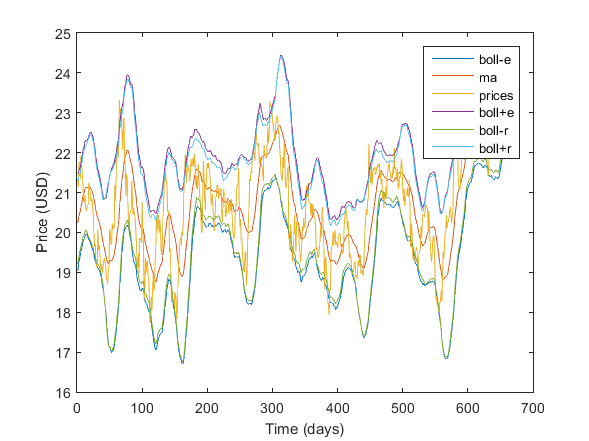
\includegraphics[width=1\textwidth]{model_vol/5}
        \caption{$\delta(t) = r\sigma_{SV}(t) - r\sigma_{STD}(t)$}
        \label{fig:diff_vol}
    \end{subfigure}
    \begin{subfigure}[t]{0.49\textwidth}
        \centering
        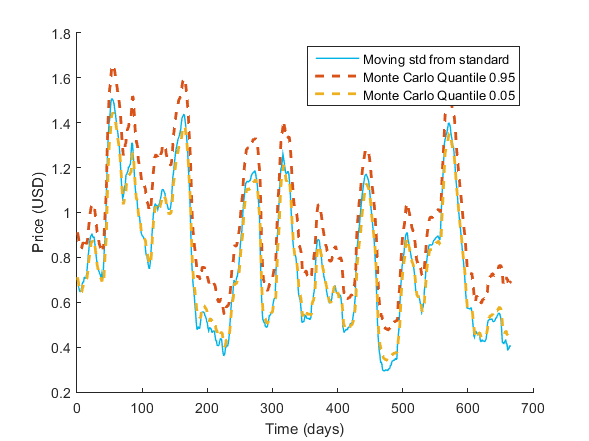
\includegraphics[width=1\textwidth]{model_vol/4}
        \caption{$r\sigma_{STD}(t)$ and estimated 90\% confidence intervals (MC)}
        \label{vol_mod_4}
    \end{subfigure}
    \begin{subfigure}[t]{0.49\textwidth}
        \centering
        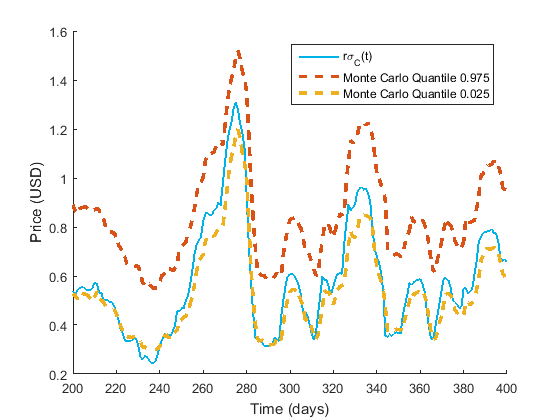
\includegraphics[width=1\textwidth]{model_vol/4_2}
        \caption{$r\sigma_{STD}(t)$ and estimated 95\% confidence intervals (MC)}
        \label{vol_mod_4}
    \end{subfigure}
    \caption{Confidence intervals of the rolling volatilities of $S_t$}
    \label{fig:rolling_vol_and_confidence_intervals}
\end{figure}

When the rolling volatilities have been estimated, the Bollinger bands can finally be computed. Equation (\ref{bolls_computations}) and (\ref{bolls_computation_sv}) are used to form the bands respectively for the standard and stochastic volatility estimators $r\sigma_{STD}(t)$ and $r\sigma_{SV}(t)$.
\begin{equation}
\label{bolls_computation_sv}
B^\pm(t,p,\alpha) = m(t,p) \pm \alpha \cdot r\sigma_{SV}(t,p)
\end{equation}
where the notations of Section \ref{sec:bollinger_bands} apply. Figure \ref{fig:bollinger_bands_sma_ema} shows the results for $p=20$ and $\alpha = 2$. The mid band was computed using a simple moving average (SMA) and an exponential moving average (EMA). Not surprisingly, the bands computed with the standard methods are narrower than the ones estimated from stochastic volatility models. It becomes now interesting to see if this more complex modelization can help build more accurate trading signals.

\begin{figure}[H]
    \centering
    \begin{subfigure}[t]{0.49\textwidth}
        \centering
        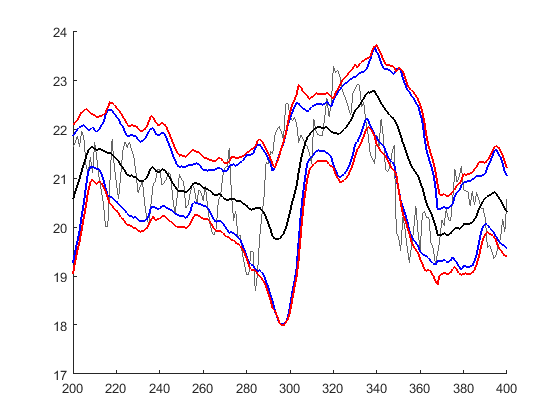
\includegraphics[width=1\textwidth]{model_vol/6}
        \caption{$(p, \alpha, t) = (20, 2.0,\text{EMA})$}
        \label{vol_mod_ema}
    \end{subfigure}
    \begin{subfigure}[t]{0.49\textwidth}
        \centering
        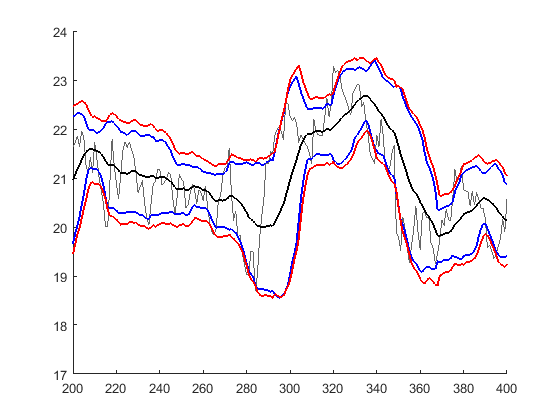
\includegraphics[width=1\textwidth]{model_vol/7}
        \caption{$(p, \alpha, t) = (20, 2.0,\text{SMA})$}
        \label{vol_mod_sma}
    \end{subfigure}
    \caption{Bollinger bands computed with $r\sigma_{STD}(t)$ (blue) and $r\sigma_{SV}(t)$ (red)}
    \label{fig:bollinger_bands_sma_ema}
\end{figure}

\section{Selection and Calibration Step}
For each training set $(\mathcal{I}_i)_{1 \leq i \leq 12}$, the cointegrated triples are formed and the models calibrated. The same sector assumption is not considered but the sets of cointegrated triples are truncated to ensure a reasonable size. Table \ref{tab:calibration_selection} summarizes the selected triples for each period and to which sector they belong. The Bollinger bands strategy with simple modelling does not require a calibration phase. The function \texttt{bollinger} from the MATLAB Financial toolbox is used to compute the three bands\footnote{For more information, the reader can consult the MATLAB documentation: \url{http://mathworks.com/help/finance/bollinger.html}}. Complex modelling requires the estimation of each parameter of model $\mathcal{M}_7$ with \textit{Particle Markov Chain Monte Carlo}. As the number of spreads is big (46484 according to Table \ref{tab:calibration_selection}), a slightly different version of Algorithm \ref{algo_pmcmc} is used (Appendix \ref{app:cauchy_pmmh}).
\begin{table}[H]
\centering
\begin{tabular}{lllll}
\hline
                              && \multicolumn{3}{l}{Sector Belonging Criterion}  \\
Period & Coint triples & All & Partial & None \\
\hline
Jan, 1 1990 - Jan, 1 1992 & 3503    & 622 (0.177) & 1637 (0.467) & 1244 (0.355) \\
Jan, 1 1992 - Jan, 1 1994 & 2147    & 323 (0.150) & 1187 (0.552)  & 637 (0.297) \\
Jan, 1 1994 - Jan, 1 1996 & 3928    & 449 (0.114) & 1748 (0.445)  & 1731 (0.440) \\
Jan, 1 1996 - Jan, 1 1998 & 4640    & 471 (0.101) & 2207 (0.475)  & 1962 (0.422) \\
Jan, 1 1998 - Jan, 1 2000 & 3254    & 285 (0.083) & 1574 (0.483)  & 1395 (0.429) \\
Jan, 1 2000 - Jan, 1 2002 & 2643    & 228 (0.085) & 1355 (0.512)  & 1060 (0.401)\\
Jan, 1 2002 - Jan, 1 2004 & 5718    & 338 (0.059) & 2340 (0.409)  & 3040 (0.531) \\
Jan, 1 2004 - Jan, 1 2006 & 3539    & 186 (0.052) & 1508 (0.426)  & 1845 (0.521) \\
Jan, 1 2006 - Jan, 1 2008 & 3541    & 159 (0.044) & 1350 (0.381)  & 2032 (0.573) \\
Jan, 1 2008 - Jan, 1 2010 & 5967    & 190 (0.031) & 2205 (0.369)  & 3572 (0.599) \\
Jan, 1 2010 - Jan, 1 2012 & 3521    & 167 (0.047) & 1147 (0.410)  & 1907 (0.541) \\
Jan, 1 2012 - Jan, 1 2014 & 4083    & 122 (0.029) & 1592 (0.389)  & 2371 (0.580) \\
\hline
Total & 46484 & 3540 (0.083) & 19850 (0.427) & 22796 (0.490) \\
\hline
\end{tabular}
\caption{Cointegrated triples selected on the in-sample sets. Percentages are shown in brackets.}
\label{tab:calibration_selection}
\end{table}

\section{HRSRI Portfolio Backtesting}

\subsection{Default Parameters}
In the first part, the tuning of the parameters is discarded and the default parameters $\theta (p=20, \alpha = 2, t = \text{EMA})$, as recommended by John Bollinger are considered. The parameters tuning phase could add a bias to the results because we aim to compare the two Bollinger bands strategies for a fixed $\theta$. The default parameters are widely used in practice among traders and it is therefore pertinent to base the comparison for those values. \\

For each period $i$ and for each strategy, the 20 best in-sample $\mathcal{SR}_{\mathcal{I}_i}$ triples are selected to compose the portfolio of the strategy. The assessment is done on the corresponding out-sample set $\mathcal{O}_i$. The procedure is explained for the period Jan, 01 2008 - Dec, 31 2009. Of the possible triples candidates, 5967 passed the cointegration tests described in Algorithm \ref{formation_spread_algorithm} (Table \ref{tab:calibration_selection}). Tables \ref{20_selected_triples_simple_bands}, \ref{20_selected_triples_complex_bands_sv} and \ref{20_selected_triples_zscore} show the 20 tradable triples used in each strategy. $\beta = (\beta_1, \beta_2, \beta_3)$ is the cointegrating vector associated to the triple. $\mathcal{SR}_\mathcal{O}$ corresponds to the Sharpe ratio on the out-sample set. The cumulative returns (CR) with costs and the number of trades are recorded on the out-sample step. A closer look shows that all the triples exhibit a very high Sharpe ratio on the in-sample period, as expected, and a lower but still promising Sharpe ratio on the out-sample period. Table \ref{tab:valuation_portfolio_2008_2009} summarizes some statistics for the three portfolios.

\renewcommand{\arraystretch}{0.8}% Wider
\begin{table}[H]
\centering
\begin{adjustwidth}{-2.6cm}{}
\begin{tabular}{llllllllllll}
\hline
Stock 1 & Stock 2 & Stock 3 & $\beta_1$ & $\beta_2$ & $\beta_3$ & $\mathcal{SR}_\mathcal{I}$ & $\mathcal{SR}_\mathcal{O}$ & \specialcell{Net\\Return} & \specialcell{Annualized\\Return} & \specialcell{Max\\Drawdown} & \specialcell{Number of\\Trades}\\ \hline
SYY  & PNC  & PRU  & 1.00 & -0.04 & -0.13 & 3.90 & 1.07 & 27394.60 & 130.45\%& 0.29 & 10 $\times$ 2\\
SEE  & SHLD  & UNM  & 1.00 & -0.21 & -0.28 & 3.75 & 1.80 & 16396.51 & 47.97\%& 0.09 & 12 $\times$ 2\\
HIG  & BCR  & BRK/B  & 1.00 & -0.65 & -1.58 & 3.55 & 0.23 & 12665.36 & 19.99\%& 0.62 & 8 $\times$ 2\\
ETFC  & DDR  & DE  & 1.00 & -0.31 & -0.47 & 3.51 & 0.87 & 13869.04 & 29.01\%& 0.29 & 10 $\times$ 2\\
FCX  & DIS  & DO  & 1.00 & -0.43 & -0.84 & 3.48 & 0.46 & 19763.68 & 73.22\%& 0.74 & 8 $\times$ 2\\
MA  & LSI  & OXY  & 1.00 & -0.22 & -0.31 & 3.47 & 0.88 & 24489.13 & 108.67\%& 0.31 & 11 $\times$ 2\\
AMT  & AMP  & CCI  & 1.00 & -0.16 & -0.49 & 3.44 & 1.14 & 15091.08 & 38.18\%& 0.14 & 11 $\times$ 2\\
TIE  & 0772031D  & CVH  & 1.00 & -0.47 & -0.24 & 3.44 & 0.34 & 10992.36 & 7.44\%& 0.19 & 10 $\times$ 2\\
SEE  & SCI  & SHLD  & 1.00 & -0.34 & -0.27 & 3.38 & 1.19 & 14839.25 & 36.29\%& 0.15 & 10 $\times$ 2\\
LUK  & MAC  & MHK  & 1.00 & -0.31 & -0.43 & 3.37 & 0.20 & 11666.71 & 12.50\%& 0.49 & 8 $\times$ 2\\
NSC  & PG  & R  & 1.00 & -0.50 & -0.37 & 3.35 & 1.12 & 32770.77 & 170.78\%& 0.48 & 12 $\times$ 2\\
FII  & FCX  & MSI  & 1.00 & -0.22 & -0.34 & 3.35 & 1.21 & 20997.83 & 82.48\%& 0.25 & 12 $\times$ 2\\
MKC  & JNJ  & KSU  & 1.00 & -0.57 & -0.06 & 3.28 & 0.00 & 9989.55 & -0.10\%& 0.22 & 10 $\times$ 2\\
SEE  & SHLD  & TSN  & 1.00 & -0.28 & -0.29 & 3.26 & 0.56 & 11882.95 & 14.12\%& 0.25 & 8 $\times$ 2\\
MA  & LSI  & PXD  & 1.00 & -0.23 & -0.24 & 3.24 & 0.34 & 12827.76 & 21.20\%& 0.35 & 10 $\times$ 2\\
JNS  & JDSU  & MDT  & 1.00 & -0.51 & -0.76 & 3.24 & 0.26 & 11255.74 & 9.42\%& 0.33 & 13 $\times$ 2\\
SYY  & PRU  & PTC  & 1.00 & -0.09 & -0.25 & 3.21 & 0.83 & 22991.15 & 97.43\%& 0.41 & 10 $\times$ 2\\
FOSL  & CMS  & COL  & 1.00 & -0.27 & -0.73 & 3.21 & 0.37 & 11676.18 & 12.57\%& 0.24 & 7 $\times$ 2\\
MTW  & MTG  & SUNE  & 1.00 & -0.08 & -0.59 & 3.21 & -0.12 & 9551.03 & -4.48\%& 0.27 & 10 $\times$ 2\\
HOG  & HNZ  & MDT  & 1.00 & -0.97 & -0.42 & 3.21 & 0.15 & 11108.11 & 8.31\%& 0.42 & 9 $\times$ 2\\
\hline
\end{tabular}
\caption{The 20 triples composing the portfolio of the simple Bollinger bands (2008-2009)}
\label{20_selected_triples_simple_bands}
\end{adjustwidth}
\end{table}


\begin{table}[H]
\centering
\begin{adjustwidth}{-2.6cm}{}
\begin{tabular}{llllllllllll}
\hline
Stock 1 & Stock 2 & Stock 3 & $\beta_1$ & $\beta_2$ & $\beta_3$ & $\mathcal{SR}_\mathcal{I}$ & $\mathcal{SR}_\mathcal{O}$ & \specialcell{Net\\Return} & \specialcell{Annualized\\Return} & \specialcell{Max\\Drawdown} & \specialcell{Number of\\Trades}\\ \hline
SYY  & PNC  & PRU  & 1.00 & -0.04 & -0.13 & 4.08 & 0.58 & 18069.64 & 60.52\%& 0.33 & 6 $\times$ 2\\
TIE  & 0772031D  & CVH  & 1.00 & -0.47 & -0.24 & 4.05 & 0.70 & 12159.16 & 16.19\%& 0.17 & 6 $\times$ 2\\
MAT  & KLAC  & KO  & 1.00 & -0.30 & -0.47 & 3.87 & 0.51 & 19505.18 & 71.28\%& 0.41 & 6 $\times$ 2\\
MTW  & MTG  & SUNE  & 1.00 & -0.08 & -0.59 & 3.66 & 0.28 & 10968.99 & 7.26\%& 0.19 & 4 $\times$ 2\\
ETFC  & ETN  & GCI  & 1.00 & -0.95 & -0.23 & 3.49 & 0.59 & 10912.62 & 6.84\%& 0.10 & 2 $\times$ 2\\
MKC  & COST  & COV  & 1.00 & -0.24 & -0.20 & 3.47 & 0.06 & 10240.28 & 1.80\%& 0.16 & 4 $\times$ 2\\
TWX  & TIF  & TNB  & 1.00 & -0.23 & -0.39 & 3.41 & 0.35 & 13045.36 & 22.84\%& 0.38 & 5 $\times$ 2\\
WY  & MET  & MHFI  & 1.00 & -0.19 & -0.44 & 3.41 & 1.04 & 23042.24 & 97.81\%& 0.30 & 8 $\times$ 2\\
CCK  & CCI  & GRA  & 1.00 & -0.25 & -0.18 & 3.38 & 0.60 & 12199.33 & 16.49\%& 0.16 & 6 $\times$ 2\\
MAT  & IP  & IR  & 1.00 & -0.19 & -0.26 & 3.38 & 0.84 & 16451.04 & 48.38\%& 0.33 & 3 $\times$ 2\\
BF/B  & BJS  & BNI  & 1.00 & -0.18 & -0.17 & 3.35 & 0.32 & 19287.20 & 69.65\%& 0.53 & 9 $\times$ 2\\
SEE  & SHLD  & WYN  & 1.00 & -0.20 & -0.22 & 3.35 & 0.85 & 11306.68 & 9.80\%& 0.08 & 4 $\times$ 2\\
INTC  & CSX  & CVG  & 1.00 & -0.41 & -0.19 & 3.21 & 0.15 & 12892.33 & 21.69\%& 0.91 & 5 $\times$ 2\\
CCK  & CHRS  & CSCO  & 1.00 & -0.03 & -0.60 & 3.14 & 0.56 & 11523.00 & 11.42\%& 0.14 & 5 $\times$ 2\\
ROP  & MTW  & MUR  & 1.00 & -0.19 & -0.34 & 3.04 & 1.46 & 46642.74 & 274.82\%& 0.79 & 5 $\times$ 2\\
HPQ  & HSP  & PPG  & 1.00 & -0.22 & -0.48 & 3.04 & 0.97 & 16047.82 & 45.35\%& 0.21 & 3 $\times$ 2\\
ETFC  & DDR  & DE  & 1.00 & -0.31 & -0.47 & 2.99 & 1.17 & 15966.98 & 44.75\%& 0.29 & 6 $\times$ 2\\
MSFT  & EL  & EMN  & 1.00 & -0.22 & -0.36 & 2.98 & 0.63 & 14874.22 & 36.55\%& 0.20 & 5 $\times$ 2\\
AA  & 0848680D  & AKS  & 1.00 & -0.09 & -0.53 & 2.96 & 0.72 & 13474.59 & 26.05\%& 0.23 & 6 $\times$ 2\\
THC  & PVH  & SIAL  & 1.00 & -0.41 & -0.42 & 2.95 & 0.93 & 12894.73 & 21.71\%& 0.14 & 8 $\times$ 2\\
\hline
\end{tabular}
\caption{The 20 triples composing the portfolio of the complex Bollinger bands (2008-2009)}
\label{20_selected_triples_complex_bands_sv}
\end{adjustwidth}
\end{table}

\begin{table}[H]
\centering
\begin{adjustwidth}{-2.6cm}{}
\begin{tabular}{llllllllllll}
\hline
Stock 1 & Stock 2 & Stock 3 & $\beta_1$ & $\beta_2$ & $\beta_3$ & $\mathcal{SR}_\mathcal{I}$ & $\mathcal{SR}_\mathcal{O}$ & \specialcell{Net\\Return} & \specialcell{Annualized\\Return} & \specialcell{Max\\Drawdown} & \specialcell{Number of\\Trades}\\ \hline
LNC  & LLTC  & MHK  & 1.00 & -0.71 & -0.79 & 4.53 & 1.73 & 47928.66 & 284.46\% & 0.27 & 8 $\times$ 2 \\
PNR  & HLS  & HNZ  & 1.00 & -0.28 & -0.66 & 4.15 & 0.66 & 14050.95 & 30.38\%& 0.20 & 4 $\times$ 2\\
NTAP  & DTV  & NEU  & 1.00 & -0.59 & -0.20 & 3.99 & 1.49 & 16051.81 & 45.38\%& 0.14 & 6 $\times$ 2\\
SLB  & CEG  & CF  & 1.00 & -0.24 & -0.44 & 3.97 & 1.08 & 30520.06 & 153.90\%& 0.98 & 3 $\times$ 2\\
L  & KSU  & MDLZ  & 1.00 & -0.44 & -0.67 & 3.95 & 0.32 & 12355.60 & 17.66\%& 0.27 & 2 $\times$ 2\\
MHFI  & MET  & NEE  & 1.00 & -0.25 & -0.56 & 3.94 & 0.64 & 18726.76 & 65.45\%& 0.35 & 5 $\times$ 2\\
EMR  & EIX  & FCX  & 1.00 & -0.52 & -0.26 & 3.91 & -0.30 & 2537.76 & -74.62\%& 0.92 & 7 $\times$ 2\\
HSH  & HRS  & OKE  & 1.00 & -0.16 & -0.41 & 3.91 & 0.74 & 15225.56 & 39.19\%& 0.23 & 4 $\times$ 2\\
ETFC  & AYE  & BCR  & 1.00 & -0.80 & -0.51 & 3.90 & 1.11 & 18337.12 & 62.52\%& 0.22 & 4 $\times$ 2\\
L  & KIM  & R  & 1.00 & -0.31 & -0.24 & 3.88 & 0.09 & 11723.15 & 12.92\%& 0.77 & 2 $\times$ 2\\
WY  & RTN  & SLM  & 1.00 & -0.60 & -0.18 & 3.87 & 1.36 & 23280.39 & 99.60\%& 0.31 & 4 $\times$ 2\\
JNS  & JDSU  & MDT  & 1.00 & -0.51 & -0.76 & 3.85 & 1.62 & 16043.91 & 45.32\% & 0.16 & 6 $\times$ 2\\
FII  & FISV  & MSI  & 1.00 & -0.67 & -0.27 & 3.78 & 0.98 & 21794.70 & 88.46\%& 0.35 & 4 $\times$ 2\\
KO  & KMX  & VIAB  & 1.00 & -0.05 & -0.26 & 3.75 & 0.63 & 14000.93 & 30.00\% & 0.18 & 5 $\times$ 2\\
SUNE  & AIG  & AIZ  & 1.00 & -0.06 & -0.53 & 3.73 & 0.94 & 14008.95 & 30.06\%& 0.16 & 3 $\times$ 2\\
HPQ  & HSP  & ITW  & 1.00 & -0.15 & -0.60 & 3.71 & 0.05 & 11105.64 & 8.29\%& 0.57 & 4 $\times$ 2\\
NI  & NU  & OMC  & 1.00 & -0.56 & -0.34 & 3.66 & 1.14 & 14343.82 & 32.57\%& 0.16 & 5 $\times$ 2\\
ETFC  & CCL  & CEG  & 1.00 & -0.90 & -0.24 & 3.63 & 0.84 & 14664.55 & 34.98\%& 0.19 & 3 $\times$ 2\\
SLM  & RX  & SWY  & 1.00 & -0.77 & -0.69 & 3.63 & -0.12 & 8622.02 & -13.77\%& 0.87 & 7 $\times$ 2\\
FCX  & DIS  & DO  & 1.00 & -0.43 & -0.84 & 3.56 & 1.11 & 40656.10 & 229.92\%& 0.53 & 5 $\times$ 2\\
\hline
\end{tabular}
\caption{The 20 triples composing the portfolio of the Z-score strategy (2008-2009)}
\label{20_selected_triples_zscore}
\end{adjustwidth}
\end{table}

\renewcommand{\arraystretch}{1}% Wider
\begin{table}[H]
\centering
\begin{tabular}{lllll}
\hline
Statistics  			& \specialcell{Bollinger\\Simple} & \specialcell{Bollinger\\Complex} & \specialcell{Z-score\\Strategy} & \specialcell{SPX\\Buy\&Hold}\\
\hline
\# of observations in the sample								    & 505        &505      & 505    & 505\\
\# of observations in $\mathcal{I}$						      & 169        &169      & 169    & 169\\
\# of days in the trading period ($\mathcal{O}$)    & 336        &336      & 336    & 336\\
\# of triples in the trading period   							& 20         &20       & 20     & N.A.\\
\# of cointegrated spreads to analyze 				      & 5967       &5967     & 5976   & N.A.\\
Average annualized return 										      & 45.83\%   &47.93\% & 62.05\%& 11.37\%\\
Annualized Sharpe ratio (w. risk free 2\%)					& 2.110       &2.227     & 2.341   & 0.656 \\
Annualized Sharpe ratio                             & 2.176      &2.293     & 2.394   & 0.470 \\
Largest daily return 											          & 3.59\%     &4.49\%  & 6.44\% & 10.78\%\\
Lowest daily return 											          & -5.04\%    &-4.45\%  & -3.47\% & -8.92\%\\
Cumulative profit on the trading period             & 61.11\%    &63.91\%& 82.74\% & 22.44\% \\
Correlation with the market returns 							  & -0.0246    &0.0348  & 0.0804 & 1\\
Skewness of the returns														  & -0.0702     &0.3212    & 0.8913 & 0.1331\\
Kurtosis of the returns														  & 7.3164     &5.5508   & 7.4581 & 6.4213 \\
Maximum Drawdown  												          & 0.0888  & 0.0839 & 0.0894 & 0.3273\\
\hline
\end{tabular}
\caption{Summary of triple trading for the period 2008-2009 on the out-sample set $\mathcal{O}$}
\label{tab:valuation_portfolio_2008_2009}
\end{table}

\begin{figure}[H]
    \centering
    \begin{subfigure}[t]{0.32\textwidth}
        \centering
        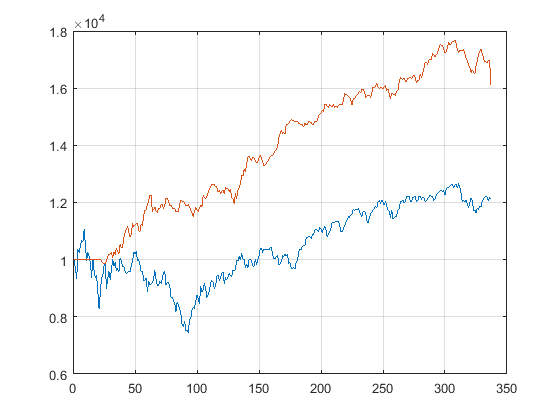
\includegraphics[width=1\textwidth]{res/strats/simple}
        \caption{Bollinger Simple}
    \end{subfigure}
    \begin{subfigure}[t]{0.32\textwidth}
        \centering
        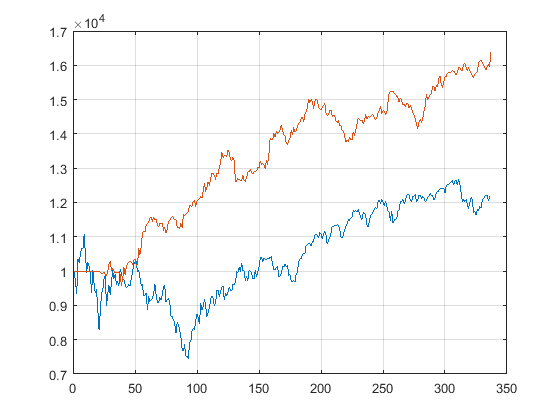
\includegraphics[width=1\textwidth]{res/strats/complex}
        \caption{Bollinger Complex}
    \end{subfigure}
    \begin{subfigure}[t]{0.32\textwidth}
        \centering
        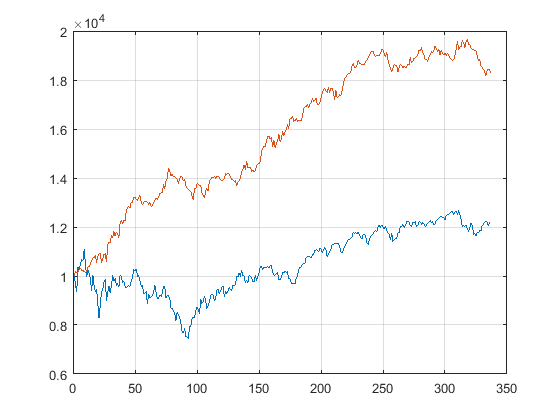
\includegraphics[width=1\textwidth]{res/strats/zscore}
        \caption{Z-score}
    \end{subfigure}
    \caption{Portfolio valuation of each strategy on the period 2008-2009. Red is the strategy. Blue is SPX.}
    \label{fig:portfolio_valuations}
\end{figure}

The valuations for the other periods are provided in Appendices \ref{app:portfolio_valuation_simple} and \ref{app:portfolio_valuation_complex}.

\subsection{Comparison of the Strategies}
At first glance, Z-score seems to be the strategy having the most promising results. One reason is that spread instruments are assumed to have a non-zero constant mean. The results are in accordance with \cite{caldeira2013} who found an average Sharpe ratio of 2 with Z-score on Brazilian markets. However, this strategy could become risky if the cointegrating property was lost. In the period Jan 2008 - Jan 2010, the Z-score strategy had two triples 7 and 19 which clearly underperformed the others. Indeed, both triples lost their cointegration property. This is why stop losses or continuous cointegration tests should be put in place to stop trading when necessary. Because none of those termination conditions have been considered in details, such a comparison could be biased and thereby we will consider the Z-score strategy as purely theoretical. Considering the Bollinger bands strategies, the complex modelling clearly smooths the cumulative returns resulting in a lower volatility, as shown by the Sharpe ratio measures. On average, the simple modelling seem to have higher cumulative returns but it comes at a much higher volatility. Thereby, the complex modelling is more accurate and less aggressive in trading. A way of making the strategy even more profitable is to tune the Bollinger parameters, as shown partially in  Section \ref{sec:optimization_bb}.

\subsection{Comparison with SPX Index}

The Bollinger bands strategies are compared to the traditional buy and hold strategy where the investor buys a basket of stocks to reproduce the S\&P500 index and holds it until the end of the period where the position is unwound. Table \ref{tab:comparison_strategies_1990_2014}, Figures \ref{fig:bollinger_bands_strategy_simple} and \ref{fig:bollinger_bands_strategy_complex} illustrate it. The Bollinger bands shows very little volatility compared to the Buy and Hold strategy of the S\&P500 index. Besides, the strategy with complex modelling accounts for a relatively low volatility for the whole period. A low correlation with the market returns confirms the market neutral property of the strategy. It is worth noticing from Table \ref{tab:comparison_strategies_1990_2014} that the excess returns are high during the crisis where the volatility was high. As highlighted by \cite{khandani2007}, the second semester of 2007 and the first semester of 2008 were hard times for quantitative investment funds. Many managers suffered losses and had to sell out their portfolios, not benefiting from the subsequent recovery. Due to its nature, the Bollinger bands is a very robust and adaptive trading indicator. Coupled with the mean-reverting properties of a spread between three stocks, the strategy could maximize the returns over the crisis periods of 2000-2002 and 2008-2010. Indeed, the returns of our strategies are correlated to the volatility of the SP\&P500 index. The complex strategy generated average excess returns of 38\% per year in out-of-samples simulations or 33\% with taking into account the calibration periods with no trading, Sharpe ratio of 2.25 and low exposure to the equity market.

\renewcommand{\arraystretch}{0.8} % Wider
\begin{table}[H]
\centering
\begin{tabular}{|l|l|l|l|l|l|}
\hline
Testing Period 336 days ($\mathcal{O}_i$) & \multicolumn{1}{|l|}{\specialcell{Sharpe\\ Ratio}} & \multicolumn{1}{|l|}{\specialcell{Max\\Drawdown}} & \multicolumn{1}{|l|}{\specialcell{Annualized\\Returns \\on $\mathcal{O}$}} & \multicolumn{1}{|l|}{\specialcell{Annualized\\ Returns \\SPX}} & \multicolumn{1}{|l|}{\specialcell{Sharpe \\Ratio \\SPX}} \\
\hline
\hline
Jan, 1 1990 - Jan, 1 1992 & \specialcell{2.210\\(1.777)} & \specialcell{0.0456\\(0.0725)}& \specialcell{16.30\%\\(19.89\%)}& 23.14\% & 1.399\\ \hline
Jan, 1 1992 - Jan, 1 1994 & \specialcell{2.715\\(2.184)} & \specialcell{0.0318\\(0.0891)} & \specialcell{26.59\%\\(46.93\%)} & 9.21\% & 1.000 \\ \hline
Jan, 1 1994 - Jan, 1 1996 & \specialcell{1.945\\(1.841)} & \specialcell{0.0363\\(0.0398)} & \specialcell{22.80\%\\(21.03\%)} & 20.74\% & 2.118 \\ \hline
Jan, 1 1996 - Jan, 1 1998 & \specialcell{1.828\\(2.071)} & \specialcell{0.0712\\(0.1182)} & \specialcell{27.61\%\\(87.12\%)} & 39.90\% & 1.384 \\ \hline
Jan, 1 1998 - Jan, 1 2000 & \specialcell{3.183\\(2.914)} & \specialcell{0.0418\\(0.0528)} & \specialcell{72.89\%\\(78.65\%)} & 31.05\% & 1.335 \\ \hline
Jan, 1 2000 - Jan, 1 2002 & \specialcell{3.563\\(0.848)} & \specialcell{0.0346\\(0.1362)} & \specialcell{49.54\%\\(19.53\%)} & -16.82\% & -0.931 \\ \hline
Jan, 1 2002 - Jan, 1 2004 & \specialcell{1.561\\(1.727)} & \specialcell{0.0355\\(0.0995)} & \specialcell{12.61\%\\(32.97\%)} & 30.99\% & 1.479 \\ \hline
Jan, 1 2004 - Jan, 1 2006 & \specialcell{2.102\\(1.014)} & \specialcell{0.0856\\(0.0674)} & \specialcell{41.64\%\\(15.04\%)} & 11.12\% & 0.997 \\ \hline
Jan, 1 2006 - Jan, 1 2008 & \specialcell{3.207\\(2.158)} & \specialcell{0.0323\\(0.0480)} & \specialcell{40.32\%\\(37.29\%)} & -0.92\% & -0.055 \\ \hline
Jan, 1 2008 - Jan, 1 2010 & \specialcell{2.293\\(2.176)} & \specialcell{0.0839\\(0.0673)}& \specialcell{47.93\%\\(45.83\%)}& 22.44\% & 0.656\\ \hline
Jan, 1 2010 - Jan, 1 2012 & \specialcell{3.526\\(3.380)} & \specialcell{0.0540\\(0.0826)}& \specialcell{82.17\%\\(114.57\%)}& 11.34\% & 0.535\\ \hline
Jan, 1 2012 - Jan, 1 2014 & \specialcell{1.424\\(1.897)} & \specialcell{0.0699\\(0.1278)}& \specialcell{16.25\%\\(46.98\%)}& 26.49\% & 1.989 \\
\hline
Total Average & \specialcell{2.4603\\(1.998)} & \specialcell{0.0518\\(0.0834)} & \specialcell{38.05\%\\(47.15\%)} & 17.39\% & 0.992\\
\hline
\end{tabular}
\caption{Statistics about the Bollinger bands strategies on the out-sample sets $\mathcal{O}$. Plain are for complex modelling and brackets are for simple modelling. }
\label{tab:comparison_strategies_1990_2014}
\end{table}

\section{Impact of Complex Modelling on the Sharpe Ratio}

\subsection{PMCMC Parameters}
Building a portfolio is a good approach to highlight the positive impact of using more complex models. Nevertheless, this cannot be considered as a full proof because the inference is only done on a small set of selected triples and not on the entire population. To reinforce our thoughts, we consider the study without any portfolios on the whole population of the cointegrated triples listed in Table \ref{tab:calibration_selection}. The model calibration is performed for each spread with the Cauchy PMCMC algorithm (Algorithm \ref{algo_pmcmc_cauchy}). Table \ref{tab:param_stats_1992_2014} presents the results of the calibration step on the in-sample sets. Some distributions are presented in Appendix \ref{app:distribution_model_parameters_m7}. The facts $\rho < 0$, $\phi_X \rightarrow 1$, $\phi_Z<\phi_X$, $\sigma_Z > \sigma_X$ are in accordance with the stylized facts and the specifications of the $\mathcal{M}_7$ (TFSVL). Not surprisingly, the two crisis periods 2000-2002 and 2008-2010 are the ones which have the highest values of $\beta$ and $\sigma_X, \sigma_Z$. Recall that $\beta$ models the amplitude of the absolute daily returns and $\sigma_X, \sigma_Z$ represent respectively the long-run and short-run volatilities. It is of common knowledge that periods of crisis come along with high absolute returns and volatility.

\renewcommand{\arraystretch}{0.9}% Wider
\begin{table}[H]
\centering
\begin{tabular}{lllllll}
\hline
\multicolumn{1}{|l|}{Period} & \multicolumn{1}{|l|}{$\mu(\phi_X)$} & \multicolumn{1}{|l|}{$\mu(\sigma_X)$} & \multicolumn{1}{|l|}{$\mu(\phi_Z)$} & \multicolumn{1}{|l|}{$\mu(\sigma_Z)$} & \multicolumn{1}{|l|}{$\mu(\beta)$} & \multicolumn{1}{|l|}{$\mu(\rho)$} \\ \hline
Jan, 1 1990 - Jan, 1 1992 &  0.9853 & 0.3590 & 0.4002 & 0.4987 & 0.4761 & -0.5256 \\
Jan, 1 1992 - Jan, 1 1994 &  0.9860 & 0.3468 & 0.4109 & 0.4737 & 0.4552 & -0.5419 \\ 
Jan, 1 1994 - Jan, 1 1996 &  0.9834 & 0.3932 & 0.4102 & 0.5243 & 0.4762 & -0.5160 \\
Jan, 1 1996 - Jan, 1 1998 &  0.9808 & 0.4560 & 0.4116 & 0.6149 & 0.5241 & -0.5673 \\
Jan, 1 1998 - Jan, 1 2000 &  0.9802 & 0.4780 & 0.4041 & 0.4041 & 0.5426 & -0.5729 \\
Jan, 1 2000 - Jan, 1 2002 &  0.9780 & 0.5204 & 0.3970 & 0.6375 & 0.5913 & -0.5654 \\
Jan, 1 2002 - Jan, 1 2004 &  0.9842 & 0.4048 & 0.3822 & 0.5600 & 0.5079 & -0.5237 \\
Jan, 1 2004 - Jan, 1 2006 &  0.9857 & 0.3759 & 0.3635 & 0.6377 & 0.5102 & -0.4270 \\
Jan, 1 2006 - Jan, 1 2008 &  0.9847 & 0.4211 & 0.3620 & 0.6905 & 0.5551 & -0.4334 \\
Jan, 1 2008 - Jan, 1 2010 &  0.9813 & 0.4795 & 0.3809 & 0.6424 & 0.5607 & -0.5078 \\
Jan, 1 2010 - Jan, 1 2012 &  0.9829 & 0.4144 & 0.3649 & 0.6558 & 0.5460 & -0.5052\\
Jan, 1 2012 - Jan, 1 2014 &  0.9865 & 0.3685 & 0.3366 & 0.6508 & 0.4909 & -0.4515\\
\hline
\end{tabular}
\caption{Means of the parameters of $\mathcal{M}_7$ per period}
\label{tab:param_stats_1992_2014}
\end{table}

%http://stattrek.com/hypothesis-test/difference-in-means.aspx?Tutorial=AP
%http://stattrek.com/online-calculator/t-distribution.aspx
\subsection{Comparison of the Sharpe Ratios}
The Sharpe ratios $\mathcal{SR}_\mathcal{O}$ statistics are presented in Table \ref{tab:sharpe_ratios_1992_2014}. The values in plain are for complex modelling and the ones in brackets for simple modelling. \textbf{It turns out that using complex modelling results in an average increase of 8.52\% in the Sharpe-Ratio.} A t-test\footnote{For more information, the reader can consult the MATLAB documentation on \url{http://mathworks.com/help/stats/ttest.html}} is conducted to assert that the pairwise difference between the means of simple and complex modelling Sharpe ratios has a mean equal to 0. With a t-score of 2.815 with 11 degrees of freedom and a pvalue of 0.0168, the Null hypothesis is rejected at the 5\% significance level. Figure \ref{fig:sr_comparison_2008_2010} shows the distributions of the Sharpe ratios with simple and complex modelling for the period 2008-2009. We can see clearly that using complex modelling leads to an improvement in this measure.


\renewcommand{\arraystretch}{0.8}% Wider
\begin{table}[H]
\centering
\begin{tabular}{|l|l|l|l|l|}
\hline
Period & \multicolumn{1}{|l|}{Mean}     & \multicolumn{1}{|l|}{Median} & \multicolumn{1}{|l|}{Min} & \multicolumn{1}{|l|}{Max} \\
\hline
\hline
Jan, 1 1990 - Jan, 1 1992 & \specialcell{0.4442\\(0.4699)} & \specialcell{0.3855\\(0.3841)}& \specialcell{-2.1859\\(-2.6415)}& \specialcell{4.2892\\(4.4382)}\\ \hline
Jan, 1 1992 - Jan, 1 1994 & \specialcell{0.5627\\(0.5844)} & \specialcell{0.5195\\(0.5353)} & \specialcell{-2.9373\\(-3.0505)} & \specialcell{3.5681\\(3.9564)} \\ \hline
Jan, 1 1994 - Jan, 1 1996 & \specialcell{ 0.6751\\(0.6219)} & \specialcell{0.6075\\(0.5751)} & \specialcell{-2.3025\\(-2.4409)} & \specialcell{4.7169\\(4.7520)} \\ \hline
Jan, 1 1996 - Jan, 1 1998 & \specialcell{ 0.4010\\(0.3596)} & \specialcell{0.3726\\(0.3705)} & \specialcell{-3.0290\\(-3.1060)} & \specialcell{4.1024\\(4.0582)} \\ \hline
Jan, 1 1998 - Jan, 1 2000 & \specialcell{ 0.2073\\(0.1601)} & \specialcell{0.1991\\(0.0959)} & \specialcell{-2.5701\\(-2.5804)} & \specialcell{4.0478\\(5.0003)} \\ \hline
Jan, 1 2000 - Jan, 1 2002 & \specialcell{ 0.4488\\(0.3212)} & \specialcell{0.4118\\(0.2567)} & \specialcell{-2.2615\\(-2.0821)} & \specialcell{3.7445\\(3.9255)} \\ \hline
Jan, 1 2002 - Jan, 1 2004 & \specialcell{ 0.5194\\(0.4646)} & \specialcell{0.5367\\(0.4736)} & \specialcell{-3.1040\\(-3.5439)} & \specialcell{4.2277\\(4.1472)} \\ \hline
Jan, 1 2004 - Jan, 1 2006 & \specialcell{ 0.5582\\(0.5185)} & \specialcell{0.5827\\(0.5214)} & \specialcell{-2.4348\\(-2.7721)} & \specialcell{4.1926\\(4.1905)} \\ \hline
Jan, 1 2006 - Jan, 1 2008 & \specialcell{ 0.4027\\(0.4089)} & \specialcell{0.3539\\(0.3878)} & \specialcell{-2.5793\\(-2.5666)} & \specialcell{4.5596\\(3.8987)} \\ \hline
Jan, 1 2008 - Jan, 1 2010 & \specialcell{0.4226\\(0.3697)} & \specialcell{0.3845\\(0.3473)}& \specialcell{-2.7525\\(-2.7811)}& \specialcell{4.0152\\(3.8975)}\\ \hline
Jan, 1 2010 - Jan, 1 2012 & \specialcell{0.6071\\(0.5296)} & \specialcell{0.5850\\(0.5020)}& \specialcell{-2.3119\\(-2.2534)}& \specialcell{4.3517\\(4.0816)}\\ \hline
Jan, 1 2012 - Jan, 1 2014 & \specialcell{0.5137\\(0.5021)} & \specialcell{0.4877\\(0.4958)}& \specialcell{-2.8241\\(-2.8924)}& \specialcell{4.8451\\(4.8451)}\\
\hline
Total Average & \specialcell{0.4802\\(0.4425)} & \specialcell{0.4521\\(0.4121)} & \specialcell{-2.6077\\(-2.7259)} & \specialcell{4.2217\\(4.2659)} \\
\hline
\end{tabular}
\caption{Statistics about $\mathcal{SR}_O$-distributions for simple and complex volatility modelling. Plain is complex model. Brackets is simple model.}
\label{tab:sharpe_ratios_1992_2014}
\end{table}

\begin{figure}[H]
\centering
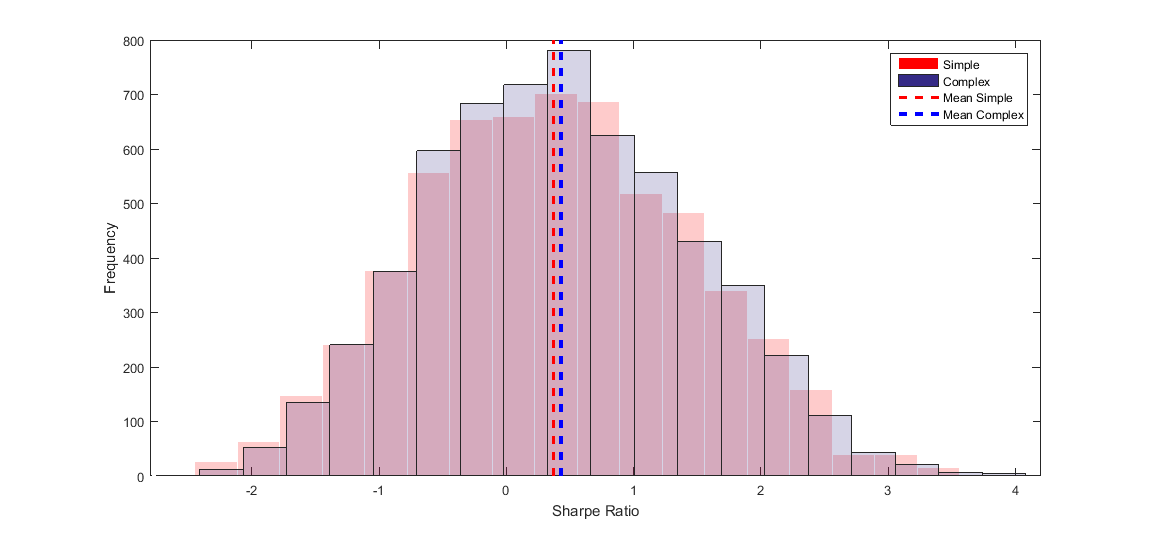
\includegraphics[width = 0.8\textwidth]{res/final_res}
\caption{Histograms of the Sharpe ratios on the out-sample set (2008-2009)}
\label{fig:sr_comparison_2008_2010}
\end{figure}

\section{Gradient and Optimization of the Bollinger Bands}
\label{sec:optimization_bb}

It becomes now interesting to see if the optimization of the default Bollinger bands parameters can lead to an increase of the profitability. \\

To have an overview, 50 spreads are randomly selected and cross validated on each set $(\mathcal{I}_i, \mathcal{O}_i)_{1 \leq i \leq 12}$. Figure \ref{fig:sharpe_ratio_topology} introduces the topology of $f$ on $\mathcal{O}$ and the gradient $\nabla f$. The type of moving average is $t = \{ EMA \}$ and is fixed throughout the study. At first sight, the region of the global maximum seems to be around $(80,1)$. In this region, the gradient seems to be fairly constant and close to 0. It gives us a hint that the bands are optimal for very large values of $p$ and for $\alpha$ being in a range [0.5,1.5]. \\

This result is in accordance with the good performance of the Z-score strategy that assumes a non-zero fixed mean. In fact, this case happens when $p \rightarrow \infty$. However, the whole population should be analyzed before making any hasty conclusions, which could be done in a future work.

\begin{figure}[H]
    \centering
    \begin{subfigure}[t]{0.32\textwidth}
        \centering
        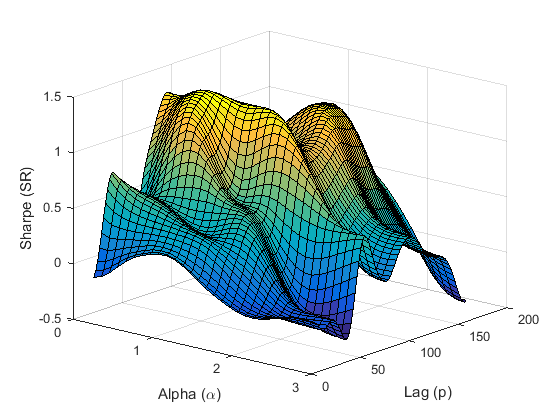
\includegraphics[width=1\textwidth]{surf/1}
        \caption{Topology of $f$ (3D)}
        \label{}
    \end{subfigure}
    \begin{subfigure}[t]{0.32\textwidth}
        \centering
        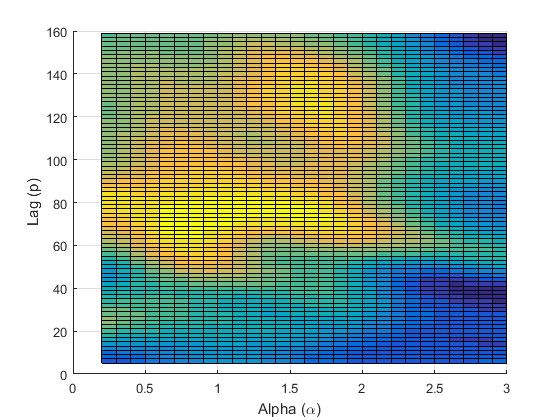
\includegraphics[width=1\textwidth]{surf/2}
        \caption{Topology of $f$ (2D)}
        \label{vol_mod_sma}
    \end{subfigure}
    \begin{subfigure}[t]{0.32\textwidth}
        \centering
        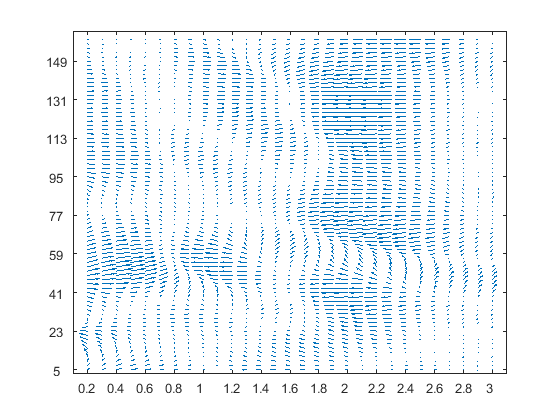
\includegraphics[width=1\textwidth]{surf/3}
        \caption{Gradient $\nabla f$}
        \label{vol_mod_sma}
    \end{subfigure}
    \caption{Detection of the stable global maximum of $f$ with $\nabla f$}
    \label{fig:sharpe_ratio_topology}
\end{figure}

\chapter{Conclusion and Future Work}

The cointegration theory has been presented and applied to financial datasets to detect cointegrated prices. These spread instruments have a mean-reverting property which is the cornerstone of many Statistical Arbitrage strategies. Of this class, triple trading has been analyzed in depth and subsequent work could be done on quadruple trading, with one being a stock index in particular. \\

We also explored the design and implementation of state-of-the-art PMCMC algorithms for the purposes of estimating latent states and static parameters in the context of Stochastic Volatility models. This class models probabilistically the volatility of the returns of financial instruments unlike GARCH family models. Parameters estimation has been demonstrated and the Two Factors Stochastic Volatility with Leverage has been selected as the best model with regard to the marginal likelihood criterion on real world data.\\

Three Statistical Arbitrage strategies based on the mean-reverting property of spread instruments have been presented: Bollinger bands with simple and complex modelling, and Z-score. While Z-score assumes a non-zero fixed mean and stochastic fixed volatility bands, the Bollinger bands assumes stochastic mean and volatility bands. Results showed that the volatility bands are slightly wider in the case of complex modelling. In order to compare the strategies, a portfolio approach is considered with a backtest window volatility of 169 days followed by a testing period of 336 days. This window is rolled 12 times to assess the performances along with some risk measures. \\

Overall, Z-score and Bollinger bands with complex modelling outperform in terms of Sharpe ratio. However, the version of Z-score implemented in the scope of this thesis is theoretical and cannot be considered as fully predictable in a practical application due to its high sensitivity to cointegration and the absence of stop loss and realtime cointegration detector. Coupled with the exhaustive study that showed that adding complex modelling results in a increase of the Sharpe ratio, the Bollinger bands strategy with this modelling is the most compelling strategy in our opinion. A future work could consist in finding the best parameters of the strategy over the whole population of spread instruments to increase the profitability while keeping a low volatility on the returns. \\

Finally and to facilitate further work on this topic, all the source code and the raw results have been published online, at an address specified in Appendix \ref{app:implementation}.

\cleardoublepage
\phantomsection
\addcontentsline{toc}{chapter}{\bibname} % Add an entry for the Bibliography in the Table of Contents
%\pagestyle{headings}

\begin{spacing}{0.9}
\bibliographystyle{abbrvnat} % set the bibliography style
\bibliography{bibtexfile} % generate the bibliography
\end{spacing}

%\cleardoublepage \fancyhead[L]{APPENDIX}
 % This line declares that you are starting the appendix.
% If you want a single Appendix and want it to be called Appendix instead of Appendix A, the following should work:
%\setcounter{secnumdepth}{-1} %This turns off automatic chapter numbering
%\chapter{Appendix}

\chapter{Appendices}

\section{Implementation}
\label{app:implementation}

\subsection{Source Code}
All the source code (algorithms, scripts, workspace variables) has been written in Octave using MATLAB 2015a. Since it is open source, it is available to everyone although you have to follow the licenses as defined in the LICENSE file.

\renewcommand{\arraystretch}{1}% Wider
\begin{table}[H]
\centering
\begin{tabular}{|ll|}
\hline
\multicolumn{1}{|l}{\textbf{Repository}}     & \multicolumn{1}{l|}{} \\ \hline
Repository URL 					   &  \url{https://github.com/philipperemy/Statistical-Arbitrage} \\
Number of commits   			 &  176 \\
Number of files   				 &  195 (MATLAB extension: .m) \\
Codebase   				         &  8727 lines\\
Author          &  Philippe Remy \\
First commit & May, 19 2015 \\
\hline
\end{tabular}
\caption{Statistics about the repository}
\label{Statistics_repository}
\end{table}

\subsection{Hierarchical Structure}

\begin{itemize}
\item \texttt{coint/} \\
Files related to cointegration tests and research on spreads (triples and quadruples).
\item \texttt{data/} \\
Contains the datasets.
\item \texttt{filters/} \\
Sequential Monte Carlo filters.
\item \texttt{helpers/} \\
Library of useful functions to manipulate data and perform common computations.
\item \texttt{likelihoods/} \\
Set of functions related to model comparisons.
\item \texttt{models/} \\
Stochastic Volatility model classes used for validation.
\item \texttt{pmcmc/} \\
Generic Particle Markov Chain Monte Carlo framework.
\item \texttt{profiling/} \\
Optimization Functions (number of particles, simulated annealing).
\item \texttt{sandbox/} \\
Experimental folder.
\item \texttt{scripts/} \\
Routine Scripts to run tests, validate models and interact with the Git remote repository.
\item \texttt{strategy/} \\
Trading framework gathering strategies (Bollinger bands, Z-score).
\item \texttt{test/} \\
Test folder. Non regression and validation tests.
\end{itemize}

\subsection{How to Get Started} 
The codebase has thousands of lines of code. Therefore, getting started is not easy.
The Particle MCMC framework, implemented for this thesis, is a highly extensible, multi-threaded and customizable framework designed to estimate parameters in non linear state-space models. The source code is provided under the MIT license and is available on Github. Contributions are welcome. \\

To define a new PMCMC scheme, the user must inherit from the base abstract class and implement the basic functions. The user must define each of its MC chains as protected member variables, define its priors and proposals distributions and finally link a Particle Filter to the class. The convention used for Particle Filter classes is to return the marginal likelihood and the estimated hidden states.

\section{Multinomial and Stratified Resampling}
\label{app:proof}

In this section, we focus on multinomial and stratified resampling. The mathematical framework is taken from \cite{douc2005}. \\

Denote by $\left( \xi_i, \omega_i \right)_{1 \leq i \leq n, t > 0}$ the set of particle positions and associated weights at time $t$. The filtration $(\mathcal{F}_t)_{t > 0}$ is used to model the information known of the particles and the weights up to time $t$. The weights are assumed to be normalized, i.e. $\forall t > 0, \sum_{i=1}^n \omega_i = 1$. Otherwise, consider $\omega_i \leftarrow \omega_i \text{ /} \sum_{j=1}^n \omega_j$. The resampling step consists in selecting new particle positions and weights $\left( \widetilde{\xi_i}, \widetilde{\omega_i} \right)_{1 \leq i \leq n}$ at time $t+1$ such that the discrepancy between the resampled weights $\widetilde{\omega_i}$ is reduced. There are many possible ways to resample. Two methods are discussed in this section: multinomial and stratified resampling. \\


Multinomial resampling is at the core of the Bootstrap method that consists in drawing, conditionally upon $\mathcal{F}_t$, the new positions $\left( \xi_i \right)_{1 \leq i \leq n}$ independently. In practice, this is achieved by repeated uses of the inversion method
\begin{itemize}
\item Draw $n$ independent uniforms $(U^i)_{1 \leq i \leq n}$ on the interval $(0, 1]$.
\item Set $I^i = D_\omega^{inv}(U^i)$ and $\widetilde{\xi_i} = \xi_{I^i}$ where $D_\omega^{inv}$ is the inverse of the cumulative distribution associated with the normalized weights $\left( \omega_i \right)_{1 \leq i \leq n}$, that is $D_\omega^{inv}(u) = i$ for $u \in \left( \sum_{j=1}^{i-1} \omega_j, \sum_{j=1}^i \omega_j \right)$. For better clarity, the function $\xi(i) = \xi_i$ is written as $\xi \circ D_\omega^{inv}(U^i)$.
\end{itemize}
This form of resampling is known as multinomial since the duplication counts are by definition distributed according to the multinomial distribution. \\


Stratified resampling is based on concepts used in survey sampling and consists in pre-partitioning the $(0,1]$ interval into $n$ disjoint sets, $(0,1] = (0, 1/n] \cup \cdots \cup (1-1/n, 1]$. The uniform random variables $U^i$ are then drawn independently in each of these sub-intervals: $U^i \sim \mathcal{U}\left( \frac{i-1}{n}, \frac{i}{n} \right)$. Then, the inversion method is used as in multinomial resampling.


\begin{proof}
For multinomial resampling, the selection indices $I^1,\cdots,I^n$ are conditionally i.i.d. given $\mathcal{F}_t$ and thus the conditional variance is given by
\begin{align*}
\var_M \left[ \frac{1}{n} \sum_{i=1}^n f(\widetilde{\xi_i}) \bigg| \mathcal{F}_t \right] &= \frac{1}{n^2} \var \left[ \sum_{i=1}^n f(\widetilde{\xi_i}) \bigg| \mathcal{F}_t \right] \\
																					  &= \frac{1}{n^2} \sum_{i=1}^n \var \left[ f(\widetilde{\xi_i}) \bigg| \mathcal{F}_t \right] \\
																					  &= \frac{1}{n} \left\{\sum_{i=1}^n \omega_i f^2(\xi_i) - n \left(\sum_{i=1}^n \omega_i f(\xi_i)\right)^2\right\} \numberthis
\end{align*}

An important result for Stratified resampling is
\begin{align*}
E \left[ \sum_{i=1}^n f(\widetilde{\xi_i})  \bigg| \mathcal{F}_t \right] &= E \left[ \sum_{i=1}^n f \circ \xi \circ D_\omega^{inv}(U^i) \bigg| \mathcal{F}_t \right] \\
																  &= \sum_{i=1}^n E \left[ f \circ \xi \circ D_\omega^{inv}(U^i) \bigg| \mathcal{F}_t \right] \\
																  &= n \sum_{i=1}^n \int_{(i-1)/n}^{i/n} f \circ \xi \circ D_\omega^{inv}(u)\text{ }du \numberthis \\
																  &= n \sum_{i=1}^n \omega_i f(\xi_i)
\end{align*}
$U^1,\cdots,U^n$ are still conditionally independent given $\mathcal{F}_t$ for the stratified resampling

\begin{align*}
\var_S \left[ \frac{1}{n} \sum_{i=1}^n f(\widetilde{\xi_i}) \bigg| \mathcal{F}_t \right] &= \frac{1}{n^2} \var \left[ \sum_{i=1}^n f(\widetilde{\xi_i}) \bigg| \mathcal{F}_t \right] \\
																					  &= \frac{1}{n^2} \sum_{i=1}^n \left\{ E \left[ f \circ \xi \circ D_\omega^{inv}(U^i)^2 \bigg| \mathcal{F}_t \right] - E \left[ f \circ \xi \circ D_\omega^{inv}(U^i) \bigg| \mathcal{F}_t \right]^2 \right\}\\
																					  &= \frac{1}{n^2} E \left[ \sum_{i=1}^n f \circ \xi \circ D_\omega^{inv}(U^i)^2 \bigg| \mathcal{F}_t \right] - \frac{1}{n^2} E \left[ f \circ \xi \circ D_\omega^{inv}(U^i) \bigg| \mathcal{F}_t \right]^2 \\
																					  &= \frac{1}{n} \sum_{i=1}^n \omega_i f^2(\xi_i) - \frac{1}{n^2} \sum_{i=1}^n \left[ n \int_{(i-1)/n}^{i/n} f \circ \xi \circ D_\omega^{inv}(u)\text{ }du\right]^2 \\
																					  &= \frac{1}{n} \sum_{i=1}^n \omega_i f^2(\xi_i) - \sum_{i=1}^n \left[ \int_{(i-1)/n}^{i/n} f \circ \xi \circ D_\omega^{inv}(u)\text{ }du\right]^2 \numberthis
\end{align*}

By Jensen's inequality,
\begin{align*}
\sum_{i=1}^n \left[ \int_{(i-1)/n}^{i/n} f \circ \xi \circ D_\omega^{inv}(u)\text{ }du\right]^2 &\geq \left[\sum_{i=1}^n \int_{(i-1)/n}^{i/n} f \circ \xi \circ D_\omega^{inv}(u)\text{ }du\right]^2 = \left[ \sum_{i=1}^n w_i f(\xi_i)\right]^2 \numberthis
\end{align*}
Finally,
\begin{equation}
\var_M \left[ \frac{1}{n} \sum_{i=1}^n f(\widetilde{\xi_i}) \bigg| \mathcal{F}_t \right] \geq \var_S \left[ \frac{1}{n} \sum_{i=1}^n f(\widetilde{\xi_i}) \bigg| \mathcal{F}_t \right] \numberthis
\end{equation}
which closes the proof.
\end{proof}

\section{Correlation Analysis of Quadruples}
\label{sec:corr_analysis_quad}
Figure \ref{dist_100_r2_quad} presents the distributions of $R^2$ for each stock sector for quadruples. The period spans the time from Jan 01, 2012 to May 27, 2013. Most distributions exhibit a bell shape with thin right tails and are therefore candidates for a filtering selection based on an arbitrary threshold $R^2_{th}$. It is worth noting that for $n=4$, each sector has its own threshold $R^2_{th}$. Table \ref{corr_quad} shows the number of quadruples before and after the filtering. $R^2_{thr}$ has been selected in such a way that roughly between 1000 and 10000 quadruples are selected for each sector for cointegration tests.

\begin{figure}[H]
\centering
    \begin{subfigure}[t]{0.23\textwidth}
        \centering
        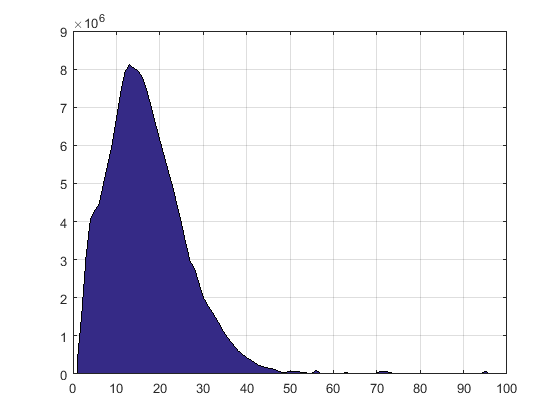
\includegraphics[width=1\textwidth]{quad/1}
        \caption{Consumer Discretionary}
    \end{subfigure}
    \begin{subfigure}[t]{0.23\textwidth}
        \centering
        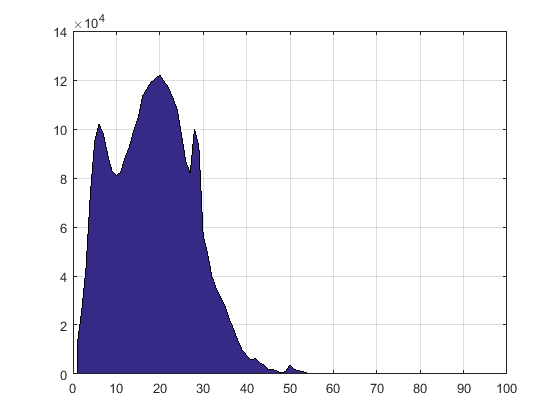
\includegraphics[width=1\textwidth]{quad/2}
        \caption{Consumer Staples}
    \end{subfigure}
    \begin{subfigure}[t]{0.23\textwidth}
        \centering
        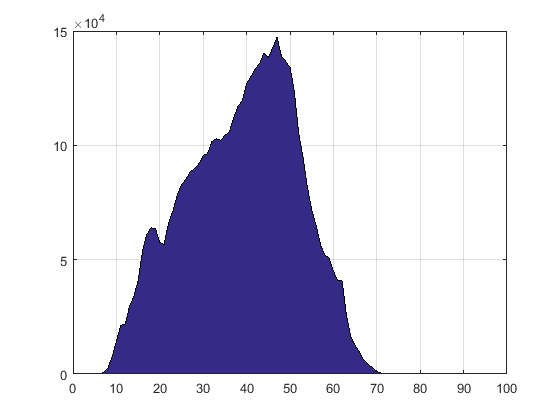
\includegraphics[width=1\textwidth]{quad/3}
        \caption{Energy}
    \end{subfigure}
    \begin{subfigure}[t]{0.23\textwidth}
        \centering
        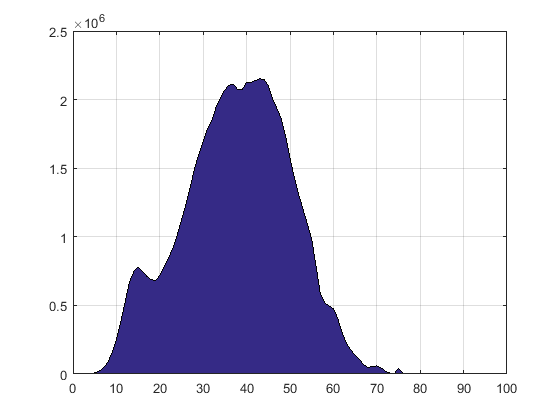
\includegraphics[width=1\textwidth]{quad/4}
        \caption{Financials}
    \end{subfigure}
    \begin{subfigure}[t]{0.23\textwidth}
        \centering
        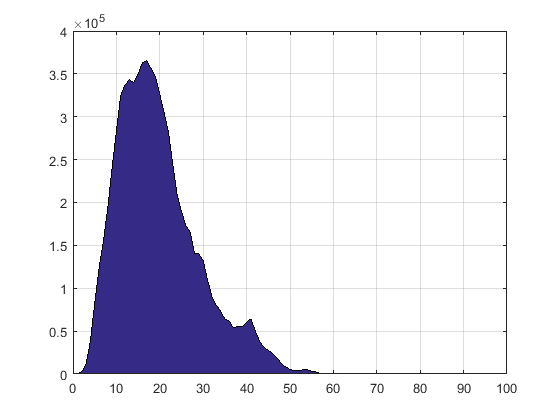
\includegraphics[width=1\textwidth]{quad/5}
        \caption{Health Care}
    \end{subfigure}
    \begin{subfigure}[t]{0.23\textwidth}
        \centering
        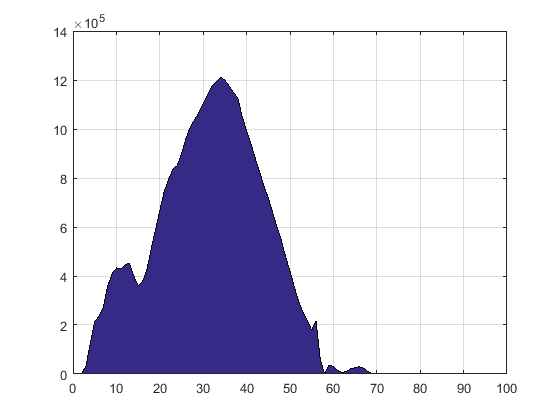
\includegraphics[width=1\textwidth]{quad/6}
        \caption{Industrials}
    \end{subfigure}
    \begin{subfigure}[t]{0.23\textwidth}
        \centering
        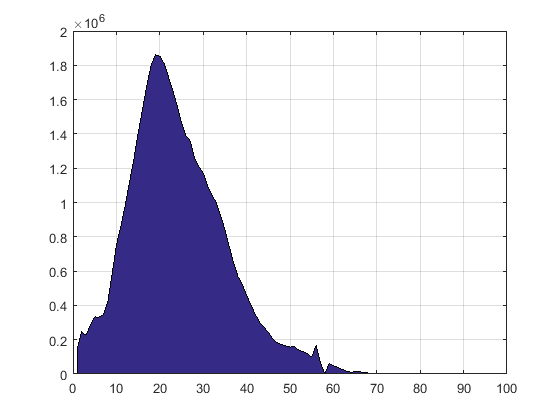
\includegraphics[width=1\textwidth]{quad/7}
        \caption{Information Technology}
    \end{subfigure}
    \begin{subfigure}[t]{0.23\textwidth}
        \centering
        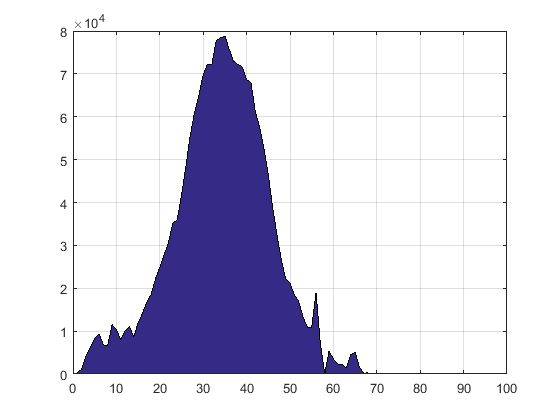
\includegraphics[width=1\textwidth]{quad/8}
        \caption{Materials}
    \end{subfigure}
    \begin{subfigure}[t]{0.23\textwidth}
        \centering
        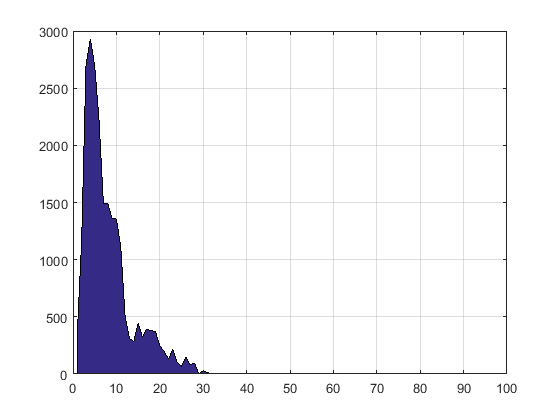
\includegraphics[width=1\textwidth]{quad/9}
        \caption{N.A.}
    \end{subfigure}
    \begin{subfigure}[t]{0.23\textwidth}
        \centering
        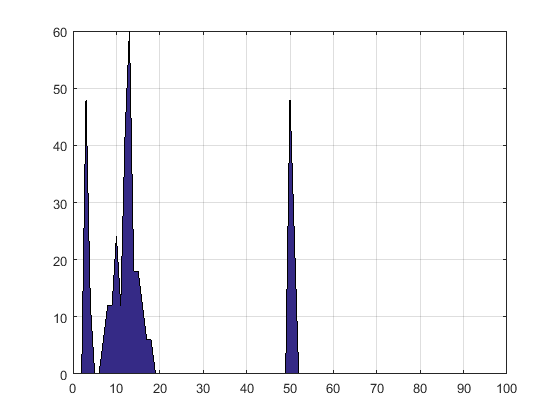
\includegraphics[width=1\textwidth]{quad/10}
        \caption{Telecommunication Services}
    \end{subfigure}
    \begin{subfigure}[t]{0.23\textwidth}
        \centering
        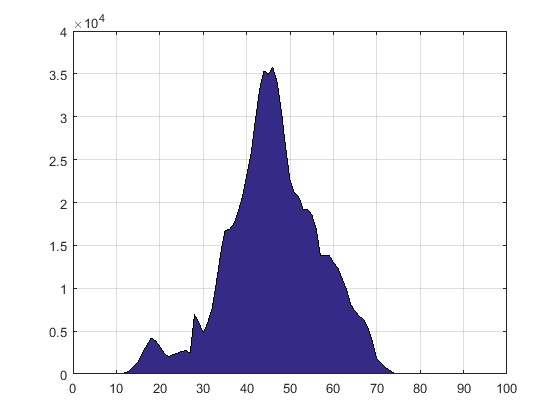
\includegraphics[width=1\textwidth]{quad/11}
        \caption{Utilities}
    \end{subfigure}
\caption{Densities of $R^2$ for the quadruples. Not all are cointegrated. Period is from Jan 01, 2012 to May 27, 2013}
\label{dist_100_r2_quad}
\end{figure}

\begin{table}[H]
\centering
\begin{tabular}{llll}
\hline
\multicolumn{1}{|l|}{Sector name}     & \multicolumn{1}{|l|}{Count before filtering} & \multicolumn{1}{|l|}{Measure $R_{thr}^2$} & \multicolumn{1}{l|}{Count after filtering} \\ \hline
Consumer Discretionary						 &  165986922 & 0.95 & 15936 \\
Consumer Staples                   &  3025246 & 0.54 & 1074\\
Energy                             &  4651592 & 0.70 & 1536\\
Financials                         &  69777874 & 0.77 & 2730\\
Health Care                        &  7567468 & 0.56 & 2982\\
Industrials                        &  36063822 & 0.70 & 1338\\
Information Technology             & 44043326 & 0.72 & 1080\\
Materials                          & 1972014 & 0.66 & 2070\\
N.A                                & 23232 & 0.21 & 1080\\
Telecommunication Services         & 360 & 0.00 & 360\\
Utilities                          & 760164 & 0.72 & 1290\\
\hline
\end{tabular}
\caption{Correlation filtering for the quadruples on Jan 01, 2012 - May 27, 2013}
\label{corr_quad}
\end{table}

\newpage
\section{Cointegration on Foreign Exchange Rates (FX)}

The dataset $\mathcal{FX}_{daily}$ presented in Section \ref{sec:presentation_data} is used in this section. Table \ref{coint_fx} presents an overview of the cointegrated prices between the different currency pairs for triple trading.

\begin{table}[H]
\centering
\begin{tabular}{llllll}
Currency 1      & Currency 2 & Currency 3 & $\beta_1$ & $\beta_2$ & $\beta_3$ \\ 
\hline
01-Jan-1999 &- 01-Jan-2001 \\
\hline
CADUSD & AUDUSD & EURUSD & 1.000000& -0.169999& 0.041106 \\
CADUSD & AUDUSD & CHFUSD & 1.000000& -0.168860& 0.050292 \\
CADUSD & EURUSD & NZDUSD & 1.000000& -0.042766& -0.136377 \\
CADUSD & EURUSD & CHFUSD & 1.000000& -0.060119& 0.070569 \\
CADUSD & NZDUSD & CHFUSD & 1.000000& -0.137284& 0.055910 \\
\hline
01-Jan-2001 &- 01-Jan-2003 \\
\hline
EURUSD & AUDUSD & GBPUSD & 1.000000& -0.243406& -0.858606 \\
EURUSD & GBPUSD & CADUSD & 1.000000& -0.942491& -0.167773 \\
CHFUSD & GBPUSD & CADUSD & 1.000000& -0.773401& -0.197333 \\
EURUSD & GBPUSD & NZDUSD & 1.000000& -0.843365& -0.251468 \\
EURUSD & GBPUSD & CHFUSD & 1.000000& -0.508161& -0.566663 \\
CHFUSD & GBPUSD & NZDUSD & 1.000000& -0.706983& -0.182011 \\
CHFUSD & CADUSD & EURUSD & 1.000000& -0.045434& -0.871733 \\
\hline
01-Jan-2003 &- 01-Jan-2005 &(Nothing)\\
\hline
01-Jan-2005 &- 01-Jan-2007 \\
\hline
EURUSD & AUDUSD & GBPUSD & 1.000000& -0.225093& -0.672751 \\
EURUSD & GBPUSD & ZARUSD & 1.000000& -0.738529& -0.102339 \\
\hline
01-Jan-2007 &- 01-Jan-2009 &(Nothing)\\
\hline
01-Jan-2009 &- 01-Jan-2011 &  (Nothing)\\
\hline
01-Jan-2011 &- 01-Jan-2013\\
\hline
GBPUSD & AUDUSD & CADUSD & 1.000000& -0.308276& -0.168456 \\
GBPUSD & CADUSD & NZDUSD & 1.000000& -0.268217& -0.227796 \\
GBPUSD & CADUSD & ZARUSD & 1.000000& -0.276975& -0.172995 \\
GBPUSD & CADUSD & CHFUSD & 1.000000& -0.432923& -0.177363 \\
\hline
\end{tabular}
\caption{Cointegration on FX Rates between Jan, 1 1999 and Jan, 1 2013}
\label{coint_fx}
\end{table}

\section{Distribution of Model Parameters for Calibration Step}
\label{app:distribution_model_parameters_m7}
\begin{figure}[H]
    \centering
    \begin{subfigure}[t]{0.32\textwidth}
        \centering
        \includegraphics[width=1\textwidth]{res/params/731_1462/1}
        \caption{$\phi_X$}
    \end{subfigure}
    \begin{subfigure}[t]{0.32\textwidth}
        \centering
        \includegraphics[width=1\textwidth]{res/params/731_1462/2}
        \caption{$\sigma_X$}
    \end{subfigure}
    \begin{subfigure}[t]{0.32\textwidth}
        \centering
        \includegraphics[width=1\textwidth]{res/params/731_1462/3}
        \caption{$\phi_Z$}
    \end{subfigure} \\
    \begin{subfigure}[t]{0.32\textwidth}
        \centering
        \includegraphics[width=1\textwidth]{res/params/731_1462/4}
        \caption{$\sigma_Z$}
    \end{subfigure}
    \begin{subfigure}[t]{0.32\textwidth}
        \centering
        \includegraphics[width=1\textwidth]{res/params/731_1462/5}
        \caption{$\beta$}
    \end{subfigure}
    \begin{subfigure}[t]{0.32\textwidth}
        \centering
        \includegraphics[width=1\textwidth]{res/params/731_1462/6}
        \caption{$\rho$}
    \end{subfigure}
    \caption{Distributions of the parameters for 2147 spreads (Jan 1992 - Jan 1994)}
    \label{fig:param_dists_1992_1994}
\end{figure}

\begin{figure}[H]
    \centering
    \begin{subfigure}[t]{0.32\textwidth}
        \centering
        \includegraphics[width=1\textwidth]{res/params/6575_7306/1}
        \caption{$\phi_X$}
    \end{subfigure}
    \begin{subfigure}[t]{0.32\textwidth}
        \centering
        \includegraphics[width=1\textwidth]{res/params/6575_7306/2}
        \caption{$\sigma_X$}
    \end{subfigure}
    \begin{subfigure}[t]{0.32\textwidth}
        \centering
        \includegraphics[width=1\textwidth]{res/params/6575_7306/3}
        \caption{$\phi_Z$}
    \end{subfigure} \\
    \begin{subfigure}[t]{0.32\textwidth}
        \centering
        \includegraphics[width=1\textwidth]{res/params/6575_7306/4}
        \caption{$\sigma_Z$}
    \end{subfigure}
    \begin{subfigure}[t]{0.32\textwidth}
        \centering
        \includegraphics[width=1\textwidth]{res/params/6575_7306/5}
        \caption{$\beta$}
    \end{subfigure}
    \begin{subfigure}[t]{0.32\textwidth}
        \centering
        \includegraphics[width=1\textwidth]{res/params/6575_7306/6}
        \caption{$\rho$}
    \end{subfigure}
    \caption{Distributions of the parameters for 5967 spreads (Jan 2008 - Jan 2010)}
    \label{fig:param_dists_2000_2002}
\end{figure}

\section{Cauchy PMMH}
\label{app:cauchy_pmmh}
In order to balance the high computational cost of estimating thousands of parameters, we derived a slightly different version of the PMMH algorithm of \cite{andrieu2010} that we named Cauchy PMMH. The purpose of Cauchy PMMH is not to sample from the posterior distributions but to estimate the parameters with MLE in the most efficient way. As the name would suggest, the algorithm is based on Cauchy sequences to assess the convergence of the conditional marginal likelihood estimator $\log \hat{p}^N_{\theta}(y_{1:T})$. A cauchy sequence is a sequence whose elements become arbitrarily close to each other as the sequence progresses. The termination criterion is satisfied when $\log \hat{p}^N_{\theta}(y_{1:T})$ has converged at precision $\epsilon$ over the last $k$ values. Algorithm \ref{algo_pmcmc_cauchy} describes it. \\

In practical applications, $N = T$, $\epsilon = 1$, $k = 50$ and $q$ is the centered multivariate normal distribution. On average, the convergence is reached for $i$ between 75 and 150, which is respectively 133x and 67x faster than the default implementation with $N = 10000$. However, this huge performance gain is balanced by the possible termination onto local maxima. Our benchmarks revealed that it is rarely the case. Initial values of $\theta$ were randomly drawn and the Cauchy PMMH always converged to the true values.

\begin{algorithm}[H]
\caption{Particle pseudo marginal Metropolis-Hastings Algorithm (Cauchy)}\label{algo_pmcmc_cauchy}
\begin{algorithmic}[1]
\Procedure{CauchyPMMH}{$y_{1:T}$, a proposal distribution $q(\cdot|\cdot)$, the number of particles $N$, precision $\epsilon$, $k$}
\State Set static parameter vector $\theta^{(1)}$ arbitrarily
\State $\hat{p}^N_{\theta^{(1)}}(y_{1:T}), \matr{x}^{*(1)}_{1:T} \gets$ Call Bootstrap Particle Filter with $(y_{1:T}, \theta^{(1)}, N)$
\State $i \gets 2$
\While{last $k$ values of $\log \hat{p}_N(y|\theta^{(i-1:k)})$ are not steady at precision $\epsilon$}
	\State Sample $\theta'$ from $q(\theta'|\theta^{(i-1)})$
	\State $\hat{p}^N_{\theta'}(y_{1:T}), \matr{x}^{*'}_{1:T}$ $ \gets$ Call Bootstrap Particle Filter with ($y_{1:T}$, $\theta'$, $N$)
	\State If,
	
	$$\frac{q(\theta^{(i-1)}|\theta')\hat{p}_N(y_{1:T}|\theta')p(\theta')}{q(\theta'|\theta^{(i-1)})\hat{p}_N(y_{1:T}|\theta^{(i-1)})p(\theta^{(i-1)})} \geq 1$$
	
	\State Set $\matr{x}^{*(i)}_{1:T} \gets \matr{x}^{'*}_{1:T},\theta^{(i)} \gets \theta', \hat{p}^N_{\theta^{(i)}}(y_{1:T}) \gets \hat{p}^N_{\theta'}(y_{1:T})$
	\State Otherwise $\matr{x}^{*(i)}_{1:T} \gets \matr{x}^{*(i-1)}_{1:T},\theta^{(i)} \gets \theta^{(i-1)}, \hat{p}^N_{\theta^{(i)}}(y_{1:T}) \gets \hat{p}^N_{\theta^{(i-1)}}(y_{1:T})$
	\State $i \gets i + 1$
\EndWhile{end}
\\
\EndProcedure
\Return $\{ \matr{x}^{*(i)}_{1:T}, \hat{\theta}_{mle} = \theta^{(i)} \}$

\end{algorithmic}
\end{algorithm}

% \begin{figure}[H]
% \centering
% \includegraphics[width = 0.7\textwidth]{convergence}
% \caption{Convergence of $\log \hat{p}_N(y|\theta^{(i)})$ on synthetic data generated from $\mathcal{M}_2$. Convergence is at $i = 80$ for $\epsilon = 2, k = 50, N = 2T$.}
% \label{fig:sr_comparison_2008_2010}
% \end{figure}

\section{Cumulative Returns for Bollinger bands Strategy with Simple modelling}
\label{app:portfolio_valuation_simple}

\begin{figure}[H]
    \centering
    \begin{subfigure}[t]{0.32\textwidth}
        \centering
        \includegraphics[width=1\textwidth]{res/backtest/1}
        \caption{Jan 1990 - Jan 1992}
    \end{subfigure}
    \begin{subfigure}[t]{0.32\textwidth}
        \centering
        \includegraphics[width=1\textwidth]{res/backtest/2}
        \caption{Jan 1992 - Jan 1994}
    \end{subfigure}
    \begin{subfigure}[t]{0.32\textwidth}
        \centering
        \includegraphics[width=1\textwidth]{res/backtest/3}
        \caption{Jan 1994 - Jan 1996}
    \end{subfigure} \\
    \begin{subfigure}[t]{0.32\textwidth}
        \centering
        \includegraphics[width=1\textwidth]{res/backtest/4}
        \caption{Jan 1996 - Jan 1998}
    \end{subfigure}
    \begin{subfigure}[t]{0.32\textwidth}
        \centering
        \includegraphics[width=1\textwidth]{res/backtest/5}
        \caption{Jan 1998 - Jan 2000}
    \end{subfigure}
    \begin{subfigure}[t]{0.32\textwidth}
        \centering
        \includegraphics[width=1\textwidth]{res/backtest/6}
        \caption{Jan 2000 - Jan 2002}
    \end{subfigure}
    \begin{subfigure}[t]{0.32\textwidth}
        \centering
        \includegraphics[width=1\textwidth]{res/backtest/7}
        \caption{Jan 2002 - Jan 2004}
    \end{subfigure}
    \begin{subfigure}[t]{0.32\textwidth}
        \centering
        \includegraphics[width=1\textwidth]{res/backtest/8}
        \caption{Jan 2004 - Jan 2006}
    \end{subfigure}
    \begin{subfigure}[t]{0.32\textwidth}
        \centering
        \includegraphics[width=1\textwidth]{res/backtest/9}
        \caption{Jan 2006 - Jan 2008}
    \end{subfigure} \\
    \begin{subfigure}[t]{0.32\textwidth}
        \centering
        \includegraphics[width=1\textwidth]{res/backtest/10}
        \caption{Jan 2008 - Jan 2010}
    \end{subfigure}
    \begin{subfigure}[t]{0.32\textwidth}
        \centering
        \includegraphics[width=1\textwidth]{res/backtest/11}
        \caption{Jan 2010 - Jan 2012}
    \end{subfigure}
    \begin{subfigure}[t]{0.32\textwidth}
        \centering
        \includegraphics[width=1\textwidth]{res/backtest/12}
        \caption{Jan 2012 - Jan 2014}
    \end{subfigure}
    \caption{Cumulative returns for Bollinger bands strategy with simple modelling on out-sample sets $\mathcal{O}$ where ratio($\mathcal{I}, \mathcal{O})$ = 1:2. Red is the strategy. Blue is SPX.}
    \label{fig:bollinger_bands_strategy_simple}
\end{figure}

\section{Cumulative Returns for Bollinger bands Strategy with Complex modelling}
\label{app:portfolio_valuation_complex}

\begin{figure}[H]
    \centering
    \begin{subfigure}[t]{0.32\textwidth}
        \centering
        \includegraphics[width=1\textwidth]{res/backtest_cpx/1}
        \caption{Jan 1990 - Jan 1992}
    \end{subfigure}
    \begin{subfigure}[t]{0.32\textwidth}
        \centering
        \includegraphics[width=1\textwidth]{res/backtest_cpx/2}
        \caption{Jan 1992 - Jan 1994}
    \end{subfigure}
    \begin{subfigure}[t]{0.32\textwidth}
        \centering
        \includegraphics[width=1\textwidth]{res/backtest_cpx/3}
        \caption{Jan 1994 - Jan 1996}
    \end{subfigure} \\
    \begin{subfigure}[t]{0.32\textwidth}
        \centering
        \includegraphics[width=1\textwidth]{res/backtest_cpx/4}
        \caption{Jan 1996 - Jan 1998}
    \end{subfigure}
    \begin{subfigure}[t]{0.32\textwidth}
        \centering
        \includegraphics[width=1\textwidth]{res/backtest/5}
        \caption{Jan 1998 - Jan 2000}
    \end{subfigure}
    \begin{subfigure}[t]{0.32\textwidth}
        \centering
        \includegraphics[width=1\textwidth]{res/backtest_cpx/6}
        \caption{Jan 2000 - Jan 2002}
    \end{subfigure}
    \begin{subfigure}[t]{0.32\textwidth}
        \centering
        \includegraphics[width=1\textwidth]{res/backtest_cpx/7}
        \caption{Jan 2002 - Jan 2004}
    \end{subfigure}
    \begin{subfigure}[t]{0.32\textwidth}
        \centering
        \includegraphics[width=1\textwidth]{res/backtest_cpx/8}
        \caption{Jan 2004 - Jan 2006}
    \end{subfigure}
    \begin{subfigure}[t]{0.32\textwidth}
        \centering
        \includegraphics[width=1\textwidth]{res/backtest_cpx/9}
        \caption{Jan 2006 - Jan 2008}
    \end{subfigure} \\
    \begin{subfigure}[t]{0.32\textwidth}
        \centering
        \includegraphics[width=1\textwidth]{res/strats/complex}
        \caption{Jan 2008 - Jan 2010}
    \end{subfigure}
    \begin{subfigure}[t]{0.32\textwidth}
        \centering
        \includegraphics[width=1\textwidth]{res/backtest_cpx/11}
        \caption{Jan 2010 - Jan 2012}
    \end{subfigure}
    \begin{subfigure}[t]{0.32\textwidth}
        \centering
        \includegraphics[width=1\textwidth]{res/backtest_cpx/12}
        \caption{Jan 2012 - Jan 2014}
    \end{subfigure}
    \caption{Cumulative returns for Bollinger bands strategy with complex modelling on out-sample sets $\mathcal{O}$ where ratio($\mathcal{I}, \mathcal{O})$ = 1:2. Red is the strategy. Blue is SPX.}
    \label{fig:bollinger_bands_strategy_complex}
\end{figure}

\end{document}
